\section{Formální jazyky, gramatiky a automaty}
\begin{quote}
\textbf{Základní pojmy teorie formálních jazyků, definice gramatiky, Chomského hiearchie gramatik. Regulární výrazy, konečné automaty, možnosti a využití regulárních jazyků. Bezkontextové gramatiky, zásobníkové automaty, vzájemný vztah bezkontextových jazyků a zásobníkových automatů.} 
\end{quote}

\subsection{Základní pojmy teorie formálních jazyků}

\begin{description}
\item[Formální jazyk] je množina řetězců nad nějakou abecedou $\Sigma$ (někdy značena $A$). 
Formální jazyk se obvykle označuje velkým písmenem, např. $L$. $L \subseteq \Sigma^*$, 
kde $\Sigma^*$ je formální jazyk nad abecedou $\Sigma$.
\item[Řetězec] je konečná posloupnost symbolů z abecedy $\Sigma$. Například, pokud $\Sigma = \{a, b\}$, pak $w = aab$ je řetězec nad $\Sigma$.
\item[Abeceda] je konečná množina symbolů, které se používí k vytváření řetězců. Například $\Sigma = \{0, 1\}$ je binární abeceda.
\textbf{Poznámka:} Abeceda může být prázdná (neobsahuje žádné řetězce) nebo může obsahovat pouze prázdný řetězec $\epsilon$ (který nemá žádné symboly).
\item[Délka řetězce] je počet symbolů v řetězci. Například délka řetězce $w = aab$ je 3.
\item[Prázdný řetězec] je řetězec, který neobsahuje žádné symboly, a označuje se $\epsilon$. Délka prázdného řetězce je 0.
\item[Prefix] řetězce $w$ je jakýkoli řetězec, který lze získat odstraněním nula nebo více symbolů z konce $w$. Například, pokud $w = aab$, pak prefixy jsou $\epsilon$, $a$, $aa$, a $aab$.
\item[Podřetězec] řetězce $w$ je jakýkoli řetězec, který lze získat odstraněním nula nebo více symbolů ze začátku či konce $w$. Například, pokud $w = aab$, pak podřetězce jsou $\epsilon$, $a$, $b$, $aa$, $ab$, a $aab$.
\item[Postfix] řetězce $w$ je jakýkoli řetězec, který lze získat odstraněním nula nebo více symbolů z začátku $w$. Například, pokud $w = aab$, pak postfixy jsou $\epsilon$, $b$, $ab$, a $aab$.
\item[Zřetězením] dvou řetězců $x$ a $y$ vznikne řetězec, který je spojením $x$ a $y$. Například, pokud $x = aa$ a $y = b$, pak zřetězení $xy$ je $aab$.
\end{description}

Překladače a interprety jsou programy, které zpracovávají formální jazyky. 
Překladač převádí zdrojový kód napsaný v jednom jazyce (např. C++) do jiného jazyka 
(např. strojový kód), zatímco interpret přímo vykonává instrukce napsané v daném 
jazyce bez předchozího překladu.

Proces překladu:
\begin{enumerate}
\item Lexikální analýza: Kontroluje jednotlivé znaky a vytváří z nich vyšší jednotky. 
Každé slovo musí být v souladu s gramatikou jazyka.
\newline
Např. \textit{0.262.154 X \space 0.262154 \checkmark}
\item Syntaktická analýza: Kontroluje správnost vyšších jednotek jazyka. 
\newline
Např. \textit{if(podmínka) then(příkaz)}
\item Sémantická analýza: Kontroluje význam vět.
\newline
Např. \textit{if(pole.length=2) then... (je pole typu array)}
\item Generování kódu: Překlad syntakticky a sémanticky správného kódu do cílového jazyka (např. strojový kód).
\end{enumerate}

\subsection{Definice gramatiky}
Gramatika je je čtveřice $G = (N, T, P, S)$, kde:
\begin{itemize}
\item $N$ je konečná množina neterminálních symbolů (neboli proměnných).
\item $T$ je konečná množina terminálních symbolů (neboli abecedy), přičemž $N \cap T = \emptyset$.
\item $P$ je konečná množina produkčních pravidel, kde každé pravidlo má tvar $\alpha \to \beta$.
\begin{itemize}
    \item levá strana $\alpha$ musí obsahovat alespoň jeden neterminální symbol z $N$.
    \item pravá strana $\beta$ může být řetězec obsahující terminální i neterminální symboly, nebo může být prázdný řetězec $\epsilon$.
    \item $(N \cup T)^*N(N \cup T)^* \times (N \cup T)^*$ 
\end{itemize}
\item $S \in N$ je startovací symbol.
\end{itemize}
Gramatika $G$ generuje jazyk $L(G)$, který je množinou všech řetězců nad abecedou $T$, 
které lze odvodit ze startovacího symbolu $S$ pomocí produkčních pravidel v $P$. 
Formálně, řetězec $w \in T^*$ patří do jazyka $L(G)$, pokud existuje posloupnost 
odvození $S \Rightarrow^* w$, kde $\Rightarrow^*$ znamená, že $w$ lze získat z $S$ 
aplikací produkčních pravidel z $P$.

\subsection{Chomského hierarchie gramatik}
Chomského hierarchie gramatik je klasifikace formálních jazyků do čtyř tříd podle složitosti gramatik, které je generují:
\begin{itemize} 
\item Typ 0: Rekurzivně spočetné jazyky, generované obecnými gramatikami bez omezení. 
(Turingovy stroje)
\item Typ 1: Kontextové jazyky, generované kontextovými gramatikami, kde pravidla mají 
tvar $\alpha \to \beta$, kde $\alpha$ je alespoň 1 neterminální symbol a $\beta$ 
není prázdný řetězec a zároveň paltí $|\alpha| \leq |\beta|$. 
 (Lineárně omezující automaty)
\item Typ 2: Bezkontextové jazyky, generované bezkontextovými gramatikami, kde 
pravidla mají tvar $A \to \alpha$, kde $A \in N$ a $\alpha \in (N \cup T)^*$. 
(Zásobníkové automaty)
\item Typ 3: Regulární jazyky, generované regulárními gramatikami, kde pravidla mají 
tvar $A \to aB$ nebo $A \to b$, kde $A, B \in N$, $a \in T^*$ a $b \in T$.
(Deterministické konečné automaty)
\end{itemize}

\begin{quotation}
\textbf{Pumping lemma:} Pro regulární a bezkontextové jazyky existují tzv. pumping lemmata, která poskytují nutnou podmínku pro to, aby jazyk byl regulární nebo bezkontextový.
\end{quotation}

\begin{figure}[htbp]
\centering

\includegraphics[width=0.25\textwidth]{chomsky-hierarchie.png}
\caption{Chomského hierarchie gramatik}
\end{figure}

\subsection{Regulární výrazy, konečné automaty, možnosti a využití regulárních \nobreak{jazyků}.}
Regulární jazyk je jazyk, který lze generovat regulární gramatikou (typ 3) nebo 
rozpoznat konečným automatem. Regulární jazyky jsou nejjednodušší třídou jazyků v
Chomského hierarchii.
Jazyky definované regulárními  výrazy jsou regulární jazyky, tj. jazyky rozpoznávané konečnými automaty. 

Tři možnosti popisu regulárních jazyků:
\begin{itemize}
\item Regulární gramatiky
\item Regulární výrazy
\item Konečné automaty
\end{itemize}

\paragraph*{Konečné automaty:} 

Konečný automat je matematický model výpočetního zařízení, které může být v jednom z 
konečného počtu stavů a přechází mezi těmito stavy na základě vstupních symbolů.
Vstup je přijat nebo zamítnut na základě toho, zda konečný automat skončí v 
akceptujícím stavu po zpracování celého vstupu. Nemá paměť pouze aktuální stav.
Konečné automaty se dělí na dva typy:
\begin{itemize}
\item Deterministické konečné automaty (DFA): Pro každý stav a každý vstupní symbol existuje
přesně jeden přechod do dalšího stavu.
\item Nedeterministické konečné automaty (NFA): Pro každý stav a každý vstupní symbol může existovat více přechodů do různých stavů.
\end{itemize}

Formálně lze konečný automat definovat jako pětici $M = (Q, T, \delta, q_0, F)$, kde:
\begin{itemize}
\item $Q$ je konečná množina stavů.
\item $T$ je konečná množina vstupních symbolů (abeceda).
\item $\delta: Q \times T \to Q$ je přechodová funkce, která určuje, do kterých stavů 
může automat přejít z daného stavu při zpracování daného vstupního symbolu.
V případě nedeterministického automatu představuje $\delta$ zobrazrní, $Q \times T \to 2^Q$.
\item $q_0 \in Q$ je počáteční stav.
\item $F \subseteq Q$ je množina akceptujících (konečných) stavů.
\end{itemize}
\begin{quote}
    Poznámka: $\delta$ je delta, $2^Q$ je množina všech podmnožin $Q$.
\end{quote}
Konečné automaty jsou ekvivalentní regulárním gramatikám, což znamená, že každý jazyk, 
který lze generovat regulární gramatikou, lze také rozpoznat konečným automatem, a 
naopak. Regulární jazyky jsou uzavřené vůči operacím sjednocení, průniku, doplňku a 
zřetězení, což z nich činí velmi užitečný nástroj pro práci s řetězci a textem.

\paragraph*{Využití regulárních jazyků:} Regulární jazyky se široce používají v 
různých oblastech informatiky, včetně:
\begin{itemize}
\item Lexikální analýza v překladačích, kde se používají k rozpoznávání tokenů v 
zdrojovém kódu.
\item Vyhledávání a manipulace s textem pomocí regulárních výrazů (regex).
\item Jednoduché stroje pro zpracování a validaci vstupů, jako jsou automaty.
\end{itemize}

\subsection{Bezkontextové gramatiky, zásobníkové automaty, vzájemný vztah bezkontextových jazyků a zásobníkových automatů}
Bezkontextové gramatiky jsou gramatiky, kde každé produkční pravidlo má 
tvar $A \to \alpha$, kde $A$ je neterminální symbol a $\alpha$ je řetězec obsahující terminální i
neterminální symboly a zároveň paltí $|\alpha| \leq |\beta|$ (tj. délka pravé strany pravidla není delší než délka levé strany). Bezkontextové jazyky jsou jazyky, které lze generovat bezkontextovými gramatikami.
Bezkontextové gramatiky jsou nejednoznačné, což znamená, že není jednoznačné které pravidlo
aplikovat pro odvození řetězce. Například, pokud máme pravidla $S \to aSb$ a $S \to \epsilon$.

\paragraph*{Zásobníkové automaty:} 

Zásobníkové automaty jsou rozšířením konečných automatů, které mají navíc zásobník pro 
ukládání a načítání symbolů. Zásobníkové automaty jsou schopné rozpoznávat bezkontextové jazyky.
Formálně lze zásobníkový automat definovat jako sedmici $M = (Q, \Sigma, \Gamma, \delta, q_0, Z_0, F)$, kde:
\begin{itemize}
\item $Q$ je konečná množina stavů.
\item $\Sigma$ je konečná množina vstupních symbolů (abeceda).
\item $\Gamma$ je konečná množina symbolů zásobníku.
\item $\delta: Q \times (\Sigma \cup \{\epsilon\}) \times \Gamma \to Q \times \Gamma^*$ je přechodová funkce, která určuje, do kterých stavů může automat přejít z daného stavu při zpracování daného vstupního symbolu a vrcholu zásobníku.

\item $q_0 \in Q$ je počáteční stav.
\item $Z_0 \in \Gamma$ je počáteční symbol zásobníku.
\item $F \subseteq Q$ je množina akceptujících (konečných) stavů.
\end{itemize}

Vztah mezi bezkontextovými jazyky a zásobníkovými automaty je takový, že každý 
bezkontextový jazyk může být rozpoznán nějakým zásobníkovým automatem, a naopak, 
každý jazyk rozpoznaný zásobníkovým automatem je bezkontextový. Tento vztah je 
formálně vyjádřen následujícími větami:
\begin{itemize}
\item Pro každý bezkontextový jazyk $L$ existuje zásobníkový automat $M$ takový, že $L = L(M)$, kde $L(M)$ je jazyk rozpoznaný automatem $M$.
\item Pro každý zásobníkový automat $M$ existuje bezkontextová gramatika $G$ taková, že $L(M) = L(G)$, kde $L(G)$ je jazyk generovaný gramatikou $G$.
\end{itemize}

\begin{quote}
\textbf{Pumping lemma:} 
Pokud je jazyk např. bezkontextový, tak každé dost dlouhé slovo v něm musí jít 
rozdělit a část toho slova se dá opakovat víckrát a pořád zůstane v daném jazyce. 
Pokud se nám pro nějaký jazyk ukáže, že takové dělení neexistuje, pak jazyk není 
bezkontextový. Typický příklad je jazyk {$a^nb^nc^n$}, který pomocí pumping lemma dokážeme, 
že není bezkontextový.
\end{quote}

\section{Teorie vyčíslitelnosti}
\begin{quote}
\textbf{Turingův stroj, varianty Turingových strojů, univerzální Turingův stroj. Rozhodnutelnost vs rozpoznatelnost jazyka. Church-Turingova teze, problém zastavení Turingova stroje a další algoritmicky nerozhodnutelné problémy.}
\end{quote}

\subsection{Turingův stroj}
Turingův stroj je abstraktní model výpočetního zařízení (vytvořen Alanem Turingem), které se skládá z nekonečné 
pásky rozdělené na buňky, hlavy, která může číst a zapisovat symboly na pásku, a 
řídící jednotky, která určuje chování stroje na základě aktuálního stavu a symbolu 
pod hlavou. Turingův stroj je schopen simulovat jakýkoli algoritmus a je považován za 
univerzální model výpočtu. Rozpoznává rekurzivně spočetné jazyky, což znamená, že může 
rozpoznat jakýkoli jazyk, pro který existuje algoritmus, ale nemusí být schopen 
rozhodnout, zda řetězec patří do jazyka nebo ne (může se dostat do nekonečné smyčky).

Turingův stroj se formálně definuje jako sedmice $M = (Q, \Sigma, \Gamma, \delta, q_0, q_{accept}, q_{reject})$, kde:
\begin{itemize}
\item $Q$ je konečná množina stavů.
\item $\Sigma$ je konečná množina vstupních symbolů (abeceda). Neobsahuje prázdný znak $\emptyset$.
\item $\Gamma$ je konečná množina symbolů pásky, pro kterou platí $\emptyset \in \Gamma$ a $\Sigma \subseteq \Gamma$.
\item $\delta: Q \times \Gamma \to Q \times \Gamma \times \{L, R\}$ je přechodová 
funkce, která určuje, kam se má hlava posunout po 
zpracování daného vstupního symbolu na pásce a jaký symbol má být zapsán na pásku.
\item $q_0 \in Q$ je počáteční stav.
\item $q_{accept} \in Q$ je akceptující stav.
\item $q_{reject} \in Q$ je zamítající stav, přičemž $q_{accept} \neq q_{reject}$.
\end{itemize}

\paragraph*{Varianty Turingových strojů:} Existují různé varianty Turingových strojů, které se liší v některých aspektech, ale všechny jsou ekvivalentní z hlediska výpočetní síly. Některé z těchto variant zahrnují:
\begin{itemize}
\item Vícepáskový Turingův stroj má na rozdíl od zde již definovaného TS k dispozici 
hned několik pásek. Každá páska má vlastní čtecí/zapisovací hlavu.
\item Nedeterministický Turingův stroj nemá jednoznačně definovanou přechodovou funkci, 
ale pracuje se zobrazením. V některých krocích výpočtu se tento výpočet dělí do více 
větví a pokud alespoň jedna větev dojde do stavu $q_{accept}$, je výpočet úspěšný. 
Lze k němu sestavit ekvivalentní deterministický Turingův stroj.
\item TS s oboustrannou páskou má pásku, která je nekonečná na obě strany, což umožňuje 
posouvat hlavu i vlevo od počáteční pozice.
\item Univerzální Turingův stroj.
\end{itemize}

\paragraph*{Univerzální Turingův stroj:} 
Univerzální Turingův stroj je Turingův stroj (UTS), který může simulovat jakýkoli 
jiný Turingův stroj na základě jeho popisu a vstupního řetězce. 
UTS dostane na pásce Gödelovo číslo (kód) jiného Turingova stroje a vstupní řetězec 
oddělený oddělovačem, a poté simuluje tento stroj na daném vstupu.
Univerzální stroj U potom simuluje činnost stroje M a pokud M slovo w přijme, 
akceptuje toto slovo i stroj U. Ne každý binární řetězec je Gödelovým číslem nějakého Turingova stroje M (101, 0101110, …)

\subsection{Rozhodnutelnost vs rozpoznatelnost jazyka}
\begin{description}
    \item[Rozpoznatelnost] jazyka znamená, že existuje Turingův stroj, který přijme 
    všechny řetězce v jazyce a buď zamítne nebo se nikdy nezastaví pro řetězce, které 
    nejsou v jazyce. Jinými slovy, jazyk je rozpoznatelný, pokud existuje algoritmus, 
    který může potvrdit, že řetězec patří do jazyka, ale nemusí být schopen potvrdit, 
    že řetězec nepatří do jazyka (může se dostat do nekonečné smyčky).
    Takový jazyk se také nazývá rekurzivně spočetný jazyk. 
    \item[Rozhodnutelnost] jazyka znamená, že existuje Turingův stroj, který přijme
    všechny řetězce v jazyce a zamítne všechny řetězce, které nejsou v jazyce. Jinými 
    slovy, jazyk je rozhodnutelný, pokud existuje algoritmus, který může potvrdit, že 
    řetězec patří do jazyka i že řetězec nepatří do jazyka (vždy se zastaví s odpovědí 
    "ano" nebo "ne").
    Takový jazyk se také nazývá rekurzivní jazyk.
\end{description}

\subsection{Church-Turingova teze}
Church-Turingova teze je tvrzení, že všechny algoritmy 
(nebo výpočty) lze provést pomocí Turingova stroje.Jinými slovy, pokud nějaký 
problém může být řešen algoritmem, pak existuje Turingův stroj, který tento problém 
může vyřešit. 
Každý jazyk, který lze popsat konečným výrazem, je rekurzivně spočetný.
Tato teze není matematicky dokázána, ale je široce přijímána v 
informatice a matematice jako základní princip pro pochopení výpočtů a algoritmů.

\subsection{Problém zastavení Turingova stroje a další algoritmicky nerozhodnutelné problémy}
Problém zastavení Turingova stroje je otázka, zda existuje algoritmus, který může 
rozhodnout, zda daný Turingův stroj zastaví na daném vstupním řetězci. Alan Turing 
dokázal, že tento problém je nerozhodnutelný, což znamená, že neexistuje žádný 
algoritmus, který by mohl univerzálně rozhodnout, zda jakýkoli Turingův stroj zastaví.

\begin{quote}
\textbf{Důkaz diagonalizační metodou:}
  Diagonalizační metodou snadno sestavíme TS X, který se ode všech strojů v tabulce bude lišit chováním na diagonále.
Takový stroj  X potom ovšem v tabulce zdánlivě chybí, ale jelikož zde máme všechny TS, dostáváme spor s předpokladem, že tabulku lze vyplnit s pomocí stroje K, který umí rozhodnout problém zastavení. 
\begin{figure}[htbp]
\centering

\includegraphics[width=0.5\textwidth]{diagonalizace.png}
\caption{Diagonalizační metoda pro důkaz nerozhodnutelnosti problému zastavení Turingova stroje}
\end{figure}
\end{quote}

\paragraph*{Další algoritmicky nerozhodnutelné problémy:} 
\begin{itemize}
    \item[Problém ekvivalence dvou Turingových strojů ] 
    \item[Problém neprázdnosti jazyka] 
    \item[Postův korespondenční problém:] Lze  ze zadané sady dominových kostek složit posloupnost, ve které je výsledný horní řetězec stejný jako řetězec dolní?
\end{itemize}
Užitečnou technikou při dokazování je redukce jednoho problému na problém jiný.
Máme-li rozhodnout, zda nějaký problém $P_1$ je či není rozhodnutelný a víme-li, že 
problém $P_0$ rozhodnutelný není, potom obvykle postupujeme následovně:
\begin{figure}[htbp]
\centering

\includegraphics[width=0.75\textwidth]{redukce.png}
\caption{Redukce jednoho problému na problém jiný}
\end{figure}

Redukovat musíme problém, o kterém víme, že není rozhodnutelný na problém, o kterém 
to chceme dokázat. Podaří-li se nám to opačně, ještě to vůbec neznamená, že náš 
problém je skutečně nerozhodnutelný. Redukci je třeba vždy dělat ze známého problému na náš.

Kromě nerozhodnutelných problémů existují i problémy Turingovsky nerozpoznatelné, 
což znamená, že neexistuje žádný Turingův stroj, který by mohl rozpoznat jazyk 
spojený s tímto problémem. Příkladem takového problému je Problém prázdnosti jazyka. Tento jazyk není 
rozpoznatelný, protože pokud by existoval Turingův stroj, který by ho rozpoznával, 
mohl by být použit k řešení (rozhodutelnosti) problému neprázdnosti jazyka, což je již dokázáno jako nemožné.

\section{Teorie složitosti}
\begin{quote}
\textbf{Časová složitost, analýza algoritmu, asymptotická složitost algoritmu. Definice tříd P a NP, polynomiální převoditelnost problémů, pojem NP úplnosti, příklady NP úplných úloh, praktické důsledky.}
\end{quote}

Složitost algoritmu se obvykle měří v závislosti na velikosti vstupu, která se 
označuje jako $n$. Dva nejčastější typy složitosti jsou časová složitost, která měří, 
jak dlouho algoritmus běží, a prostorová složitost, která měří, kolik paměti 
algoritmus potřebuje.

\subsection{Časová složitost, analýza algoritmu, asymptotická složitost algoritmu:} 
Časová složitost algoritmu je měřítkem toho, jak se čas potřebný k provedení algoritmu zvyšuje s velikostí vstupu.
Nejčastěji se používá asymptotická notace, která popisuje chování algoritmu pro velké hodnoty $n$. Nejčastější asymptotické notace jsou:
\begin{itemize}
\item $O(f(n))$: Horní mez, která říká, že algoritmus běží nejvýše v čase $f(n)$ pro dostatečně velké $n$. (O)
\item $\Omega(f(n))$: Dolní mez, která říká, že algoritmus běží nejméně v čase $f(n)$ pro dostatečně velké $n$. (Omega)
\item $\Theta(f(n))$: Přesná asymptotická složitost, která říká, že algoritmus běží v čase $f(n)$ pro dostatečně velké $n$. (Theta)
\end{itemize}

Nejedná se o přesné měření času, ale spíše o způsob, jak popsat růst složitosti 
algoritmu v závislosti na velikosti vstupu. Například algoritmus s časovou 
složitostí $O(n^2)$ bude běžet nejvýše v čase, který je úměrný druhé mocnině 
velikosti vstupu. 

Analýza algoritmu zkoumá jak je algoritmus efektivní z hlediska času a prostoru.
Provádí se nezávisle na konkrétní implementaci a zaměřuje se na obecné chování algoritmu.

Typy časové složitosti zahrnují:
\begin{itemize}
\item Konstantní čas $O(1)$: Algoritmus běží v konstantním čase, bez ohledu na velikost vstupu.
\item Logaritmický čas $O(\log n)$: Algoritmus běží v čase, který roste logaritmicky s velikostí vstupu.
\item Lineární čas $O(n)$: Algoritmus běží v čase, který roste lineárně s velikostí vstupu.
\item Kvadratický čas $O(n^2)$: Algoritmus běží v čase, který roste kvadraticky s velikostí vstupu.
\item Polynomiální čas $O(n^k)$: Algoritmus běží v čase, který roste polynomiálně s velikostí vstupu, kde $k$ je konstanta.
\item Exponenciální čas $O(2^n)$: Algoritmus běží v čase, který roste exponenciálně s velikostí vstupu. (NP)
\item Faktoriální čas $O(n!)$: Algoritmus běží v čase, který roste faktoriálně s velikostí vstupu. (NP)
\item Superexponenciální čas $O(n^n)$: Algoritmus běží v čase, který roste superexponenciálně s velikostí vstupu. (NP)
\end{itemize}

\subsection{Definice tříd P a NP}
\paragraph*{Třída P:} Třída P je třída všech jazyků, které jsou rozhodnutelné deterministickým Turingovým strojem 
v polynomiálním čase. V podstatě odpovídá třídě úloh, které jsou realisticky řešitelné 
na počítači. Příklady úloh v P zahrnují: třídění seznamu čísel, aritmetické operace 
(sčítání, násobení, dělení), násobení matic, nejkratší cesta v grafu 
(Dijkstraův algoritmus), průměr, medián a modus, atd.

\paragraph*{Třída NP:} Třída NP (NPTIME) je třída jazyků, pro které existuje 
verifikační algoritmus pracující v polynomiálně omezeném čase.
Jazyk patří do třídy NP (NPTIME) právě tehdy, když je rozhodnutelný v polynomiálně 
omezeném čase nějakým nedeterministickým Turingovým strojem. Příklady úloh v NP 
zahrnují: izomorfismus grafů, diskrétní logaritmus, faktorování velkých čísel, atd.

Všechny úlohy v P jsou také v NP, protože deterministický Turingův stroj je 
speciálním případem nedeterministického Turingova stroje. Nicméně, není známo, zda 
všechny úlohy v NP jsou také v P, což je známé jako problém P vs NP.

Zatímco problémy z třídy P jsou „rychle“ rozhodnutelné, problémy z NP jsou pouze 
„rychle“ verifikovatelné. 

\begin{figure}[htbp]
\centering

\includegraphics[width=0.5\textwidth]{P-NP.png}
\caption{Vztah mezi třídami P, NP, NP-úplné}
\end{figure}

\subsection{Polynomiální převoditelnost problémů}
Polynomiální převoditelnost problémů je koncept, který se používá k porovnání 
složitosti různých problémů. Říkáme, že problém $A$ je polynomiálně převoditelný na 
problém $B$ (označujeme jako $A \leq_p B$), pokud existuje polynomiální algoritmus, 
který může převést instance problému $A$ na instance problému $B$.
Polynomiální převoditelnost se používá k určení, zda je problém $A$ stejně těžký jako 
problém $B$. Pokud $A \leq_p B$ a $B$ je v NP, pak $A$ je také v NP. Pokud navíc $B$ 
je NP-úplný, pak $A$ je také NP-úplný.

\subsection{NP-úplnost}
Obtížnost některých problémů z třídy NP je stejná v tom smyslu, že nalezení „rychlého“ 
algoritmu pro řešení kterékoliv z těchto úloh, by znamenalo nalezení „rychlého“ 
algoritmu pro všechny úlohy z této specifické třídy.
Problém je NP-úplný, pokud je v NP a každý problém v NP lze polynomiálně převést 
na tento problém.
Pokud by byl nalezen algoritmus, který by řešil problém z třídy NP-úplných úloh v 
polynomiálním čase, pak by všechny problémy v NP mohly být řešeny v polynomiálním 
čase, což by znamenalo, že P = NP.
Příklady NP-úplných úloh zahrnují: problém splnitelnosti logických formulí (SAT), existence
kliky, problém barvení grafu, problém nezávislé množiny, problém obchodního cestujícího, atd.

\paragraph*{Praktické důsledky:}
Pokud P = NP, znamenalo by to, že všechny problémy v NP, včetně těch, které jsou 
považovány za velmi obtížné (jako je faktorování velkých čísel), by mohly být řešeny 
efektivně. To by mělo obrovské důsledky pro kryptografii, optimalizaci a mnoho dalších 
oblastí informatiky a matematiky. Na druhou stranu, pokud P $\neq$ NP, znamenalo by 
to, že existují problémy, které jsou inherentně obtížné a nelze je řešit efektivně.

\section{Algoritmy a jejich složitosti}
\begin{quote}
\textbf{Hledání minimální kostry v grafu, artikulace, mosty, bloky v grafu, algoritmus na vyhledávání artikulací a bloků v grafu. Bipartitní grafy, párování v grafu, přiřazovací problém. Úloha čínského pošťáka.}
\end{quote}

\subsection{Hledání minimální kostry v grafu}
Minimální kostra (nebo minimální kostrový strom) v grafu je podgraf, který je stromem 
(tj. je acyklický a souvislý) a má minimální možnou cenu (součet cen hran) mezi všemi 
možnými kostrami grafu. Pro souvislé neorientované grafy s ohodnocenýmy hranami. Využívá
se například v síťových návrzích, kde je potřeba minimalizovat náklady na propojení 
všech uzlů.
Podmínky kostry:
\begin{itemize}
\item Graf musí být souvislý.
\item Graf neobsahuje cykly.
\item Graf obsahuje všechny vrcholy původního grafu.
\item Součet cen hran v kostře je minimální.
\item Počet hran v kostře je vždy $|V| - 1$, kde $|V|$ je počet vrcholů v grafu.
\end{itemize}

\paragraph*{Algoritmy pro hledání minimální kostry:}
\begin{itemize}
\item \textbf{Jarníkův algoritmus (Primův algoritmus)} -- využívá prioritní frontu pro efektivní 
výběr nejlevnější hrany. Složitost: 
\begin{itemize}
    \item $O(E \log V)$ s použitím binární haldy.
    \item $O(E + V \log V)$ s použitím Fibonacciho haldy
    \item $O(V^2)$ s použitím jednoduché matice sousednosti.
\end{itemize}
E je počet hran a V je počet vrcholů v grafu.
\begin{enumerate}
    \item Začneme s prázdnou kostrou a zvolíme libovolný počáteční vrchol.
    \item Opakovaně přidáváme nejlevnější hranu, která spojuje vrchol v kostře s 
    vrcholem mimo kostru, dokud nejsou všechny vrcholy zahrnuty.
\end{enumerate}

\item \textbf{Borůvkův algoritmus} -- Složitost: $O(E \log V)$, kde E je počet hran a V je počet vrcholů v grafu.
\begin{enumerate}
    \item Každý vrchol začíná jako samostatná komponenta.
    \item V každém kroku pro každou komponentu najdeme nejlevnější hranu, která ji spojuje s jinou komponentou. Všechny tyto hrany přidáme do kostry (duplicity se odstraní).
    \item Pokračujeme, dokud není kostra kompletní (všechny vrcholy jsou v jedné komponentě).
\end{enumerate}

\item \textbf{Kruskalův algoritmus} -- Složitost: $O(E \log E)$, kde E je počet hran v 
grafu. Pokud jsou hrany již seřazeny, složitost je $O(E \alpha(V))$, kde $\alpha$ je 
inverzní Ackermannova funkce, která roste velmi pomalu a pro všechny praktické účely 
lze považovat za konstantu. (téměř lineární čas)
\begin{enumerate}
    \item Seřadíme všechny hrany grafu vzestupně podle jejich cen.
    \item Postupně procházíme hrany a každou přidáme do kostry, pokud její přidání nevytvoří cyklus (používáme strukturu \textit{Disjoint Set Union} pro sledování komponent).
    \item Pokračujeme, dokud kostra neobsahuje $|V| - 1$ hran.
\end{enumerate}
\end{itemize}

\subsection{Artikulace}
Artikulace (neboli artikulační body) v grafu jsou vrcholy, které, pokud jsou 
odstraněny, způsobí, že graf se stane nesouvislým. Jinými slovy, artikulační bod je 
vrchol, jehož odstranění zvýší počet komponent grafu. Artikulace jsou důležité pro 
analýzu struktury grafu a pro identifikaci kritických bodů v síti.

\paragraph*{Algoritmus pro hledání artikulací:}
\begin{itemize}
    \label{para:artikulace}
\item \textbf{Tarjanův algoritmus pro artikulace} -- Složitost: $O(V + E)$, kde $V$ je počet vrcholů a $E$ je počet hran.
\begin{enumerate}
    \item Provedeme prohledávání do hloubky (DFS). Každému vrcholu $u$ přiřadíme: 
    \begin{itemize}
        \item \textit{disc[u]}: čas (pořadí) objevení vrcholu v rámci DFS.
        \item \textit{low[u]}: nejmenší \textit{disc} dosažitelný z $u$ nebo jeho potomků pomocí nejvýše jedné zpětné hrany.
    \end{itemize}
    \item Vrchol $u$ je artikulací, pokud splňuje jednu z podmínek:
    \begin{itemize}
        \item $u$ je kořenem DFS stromu a má v tomto stromě \textbf{více než jednoho přímého potomka}.
        \item $u$ není kořenem a má přímého potomka $v$ takového, že $low[v] \geq disc[u]$. (To znamená, že z podstromu vrcholu $v$ nevede žádná zpětná hrana do $u$ nebo výše.)
    \end{itemize}
\end{enumerate}
\end{itemize}

\subsection{Mosty v grafu}
Mosty (neboli hrany, které jsou mosty) v grafu jsou hrany, které, pokud jsou 
odstraněny, způsobí, že graf se stane nesouvislým. Jinými slovy, most je hrana, jejíž 
odstranění zvýší počet komponent grafu. Mosty jsou důležité pro analýzu struktury 
grafu a pro identifikaci kritických spojení v síti.

\paragraph*{Algoritmus pro hledání mostů:}
\begin{itemize}
\item \textbf{Tarjanův algoritmus pro mosty} -- Složitost: $O(V + E)$, kde $V$ je počet vrcholů a $E$ je počet hran.
\begin{enumerate}
    \item Provedeme prohledávání do hloubky (DFS). Každému vrcholu $u$ přiřadíme: 
    \begin{itemize}
        \item \textit{disc[u]}: čas objevení vrcholu v rámci DFS.
        \item \textit{low[u]}: nejmenší \textit{disc} dosažitelný z $u$ nebo jeho potomků pomocí zpětných hran (\textbf{přitom ignorujeme hranu, po které jsme do $u$ přišli z rodiče}).
    \end{itemize}
    \item Hrana $(u, v)$, kde $v$ je potomek $u$ v DFS stromu, je mostem, pokud platí:
    $low[v] > disc[u]$
    \item Algoritmus takto projde celý graf a identifikuje všechny mosty.
\end{enumerate}
\end{itemize}

\subsection{Bloky v grafu}
Bloky v grafu jsou maximální souvislé podgrafy, které po odstranění libovolného 
vrcholu zůstanou souvislé. Jinými slovy, blok je buď maximální podgraf bez 
artikulačních bodů, nebo jedna samostatná hrana (most). Bloky jsou klíčové pro 
analýzu robustnosti neorientovaných grafů, protože identifikují části sítě, které 
drží pohromadě i při výpadku jednoho uzlu.

\paragraph*{Algoritmus pro hledání bloků:}
\begin{itemize}
\item \textbf{Tarjanův algoritmus pro bloky} -- Složitost: $O(V + E)$, kde $V$ je počet vrcholů a $E$ je počet hran.
\begin{enumerate}
    \item Provedeme prohledávání do hloubky (DFS). Každému vrcholu $u$ přiřadíme 
    hodnoty \textit{disc[u]} a \textit{low[u]} (stejně jako u hledání 
    \hyperref[para:artikulace]{artikulací}).
    \item Během průchodu DFS ukládáme každou prošlou hranu na \textbf{zásobník}.
    \item Když se v rekurzi vracíme z vrcholu $v$ do $u$ a zjistíme, že je splněna podmínka artikulace ($low[v] \geq disc[u]$):
    \begin{itemize}
        \item Právě jsme našli nový blok.
        \item Ze zásobníku hran postupně vybíráme (pop) všechny hrany až po hranu $(u, v)$. Tyto hrany tvoří jeden blok (2-souvislou komponentu).
    \end{itemize}
    \item Po skončení DFS jsou všechny hrany rozděleny do příslušných bloků.
\end{enumerate}
\end{itemize}

\begin{quote}
\textbf{Poznámka k implementaci Tarjanových algoritmů:} Při DFS se hodnoty \textit{disc} (čas objevení) nastavují při cestě dolů (vstup do vrcholu). Hodnoty \textit{low} a vyhodnocení podmínek (pro artikulace, mosty i bloky) se provádějí při návratu z rekurze (backtracking).
\end{quote}

\subsection{Bipartitní grafy}
Bipartitní graf je graf, jehož vrcholy lze rozdělit do 
dvou disjunktních množin $U$ a $V$ tak, že každá hrana spojuje vrchol z $U$ s vrcholem 
z $V$. Jinými slovy, neexistují hrany mezi vrcholy v rámci stejné množiny. Bipartitní 
grafy se často používají k modelování vztahů mezi dvěma různými skupinami objektů, 
například studentů a kurzů, zaměstnanců a projektů, atd.

\subsection{Párování v grafu} 
Párování v grafu (matching) je množina nezávislých hran, tedy hran, které nemají žádný společný vrchol. V bipartitních grafech se párování často používá k řešení problémů přiřazení. Například, pokud máme bipartitní graf, kde jedna množina vrcholů reprezentuje zaměstnance a druhá projekty, párování přiřazuje zaměstnance k projektům tak, aby každý zaměstnanec pracoval maximálně na jednom projektu a každý projekt měl maximálně jednoho zaměstnance.

\begin{itemize}
\item \textbf{Maximální párování (Maximal matching):} Párování, ke kterému již není možné přidat žádnou další hranu, aniž by se porušila podmínka, že žádné dvě hrany nesmí sdílet vrchol.
\item \textbf{Největší párování (Maximum matching):} Párování, které obsahuje absolutně největší možný počet hran v daném grafu.
\item \textbf{Perfektní (úplné) párování:} Speciální případ největšího párování, které pokrývá všechny vrcholy grafu (každý vrchol je incidentní s přesně jednou hranou z párování).
\end{itemize}

\begin{figure}[htbp]
    \centering
    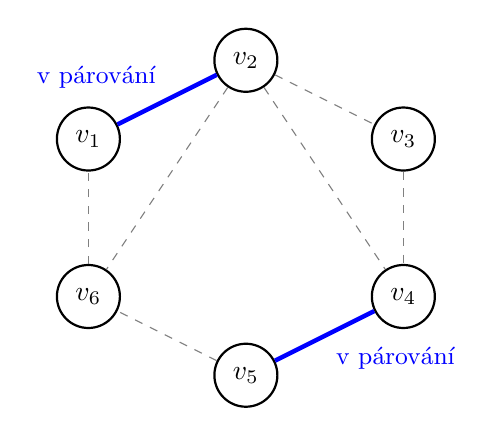
\begin{tikzpicture}[
        vertex/.style={circle, draw, minimum size=8mm, thick, fill=white},
        matched_edge/.style={blue, ultra thick},
        normal_edge/.style={gray, thin, dashed}
    ]

    % Rozmístění vrcholů obecného grafu pomocí souřadnic (x, y)
    \node[vertex] (v1) at (0, 2) {$v_1$};
    \node[vertex] (v2) at (2, 3) {$v_2$};
    \node[vertex] (v3) at (4, 2) {$v_3$};
    \node[vertex] (v4) at (4, 0) {$v_4$};
    \node[vertex] (v5) at (2, -1) {$v_5$};
    \node[vertex] (v6) at (0, 0) {$v_6$};

    % Vykreslení běžných hran (šedé, přerušované)
    \draw[normal_edge] (v2) -- (v3);
    \draw[normal_edge] (v3) -- (v4);
    \draw[normal_edge] (v5) -- (v6);
    \draw[normal_edge] (v6) -- (v1);
    
    % Vnitřní hrany (tvoří např. trojúhelníky v1-v2-v6, takže graf není bipartitní)
    \draw[normal_edge] (v2) -- (v6);
    \draw[normal_edge] (v2) -- (v4);

    % Vykreslení hran v párování (modré, tlusté plné čáry)
    \draw[matched_edge] (v1) -- (v2) node[midway, above left, text=blue, font=\small] {v párování};
    \draw[matched_edge] (v4) -- (v5) node[midway, below right, text=blue, font=\small] {v párování};

    \end{tikzpicture}
    \caption{Princip párování na obecném grafu. Modré hrany $(v_1, v_2)$ a $(v_4, v_5)$ tvoří párování, protože nemají žádný společný vrchol. Vrcholy $v_3$ a $v_6$ jsou volné. Toto párování je \textbf{maximální} (žádnou další hranu nelze přidat, aniž by sdílela vrchol s modrými), ale není \textbf{největší} (šlo by vybrat např. hrany $(v_6, v_1)$, $(v_2, v_3)$ a $(v_4, v_5)$, čímž by vzniklo perfektní párování velikosti~3).}
    \label{fig:parovani_obecny}
\end{figure}

\paragraph*{Algoritmy pro hledání párování v bipartitním grafu:}
\begin{itemize}
\item \textbf{Hopcroft-Karpův algoritmus} -- Složitost: $O(\sqrt{V} E)$, kde $V$ je počet vrcholů a $E$ je počet hran. Efektivní algoritmus pro hledání \textbf{největšího párování}.
\begin{enumerate}
    \item Provedeme prohledávání do šířky (BFS) ze všech aktuálně volných (nespárovaných) vrcholů v množině $U$. Cílem je vytvořit vrstevnatý graf a najít nejkratší cesty k volným vrcholům v množině $V$.
    \item Pokud BFS nenajde žádný dosažitelný volný vrchol ve $V$, algoritmus končí a aktuální párování je \textbf{největší}.
    \item Pro každý volný vrchol z $U$ provedeme prohledávání do hloubky (DFS) podél vrstev nalezených pomocí BFS. Hledáme \textit{zlepšující (augmentující) cestu} -- cestu, která střídá hrany mimo párování a v párování a začíná i končí ve volném vrcholu.
    \item Pokud najdeme zlepšující cestu, aktualizujeme párování přepnutím (symetrickou diferencí). Hrany na cestě, které byly v párování, z něj vyjmeme, a ty, které v něm nebyly, do něj přidáme. Tím se velikost párování zvětší o 1.
    \item Opakujeme tento proces od bodu 1, dokud lze nacházet zlepšující cesty.
\end{enumerate}

\item \textbf{Hladový (Greedy) algoritmus} -- Složitost: $O(V + E)$. Tento algoritmus slouží jako rychlá heuristika. (Nezaručuje největší párování, ale je velmi rychlý a jednoduchý.)
\begin{enumerate}
    \item Projdeme všechny hrany grafu. Pro každou hranu $(u, v)$ zkontrolujeme, zda jsou oba vrcholy $u$ a $v$ volné (nespárované).
    \item Pokud ano, přidáme hranu $(u, v)$ do párování a oba vrcholy označíme jako spárované.
    \item Pokračujeme, dokud neprojdeme všechny hrany.
    \item Výsledkem je vždy \textbf{maximální} párování, ale ne nutně \textbf{největší}. Nemusí být optimální, protože brzkým výběrem hrany můžeme zablokovat dlouhé zlepšující cesty. Je ovšem garantováno, že velikost tohoto párování je alespoň poloviční oproti největšímu možnému párování.
\end{enumerate}
\end{itemize}

\subsection{Přiřazovací problém}
Přiřazovací problém je speciální případ problému párování v bipartitním grafu, kde 
máme dvě množiny vrcholů (například pracovníci a úkoly) a každá hrana mezi nimi má 
přiřazenou cenu (náklad). Cílem je najít perfektní párování, které minimalizuje celkovou cenu 
přiřazení.

\paragraph*{Algoritmus pro řešení přiřazovacího problému:}
\begin{itemize}
\item \textbf{Maďarský algoritmus} (také známý jako Kuhn-Munkresův algoritmus) -- Složitost: $O(V^3)$, kde $V$ je počet vrcholů v jedné partitě (předpokládáme, že obě množiny mají stejný počet vrcholů, reprezentováno maticí $V \times V$). Tento algoritmus efektivně řeší problém přiřazení a zaručuje nalezení optimálního řešení.
\begin{enumerate}
    \item Vytvoříme nákladovou matici, kde řádky reprezentují jednu množinu (např. pracovníky) a sloupce druhou množinu (např. úkoly). Každá buňka obsahuje cenu přiřazení.
    \item \textbf{Redukce řádků:} Pro každý řádek najdeme nejmenší hodnotu a odečteme ji od všech hodnot v tomto řádku.
    \item \textbf{Redukce sloupců:} Pro každý sloupec najdeme nejmenší hodnotu a odečteme ji od všech hodnot v tomto sloupci.
    \item Pokusíme se najít perfektní párování výhradně pomocí nulových položek v 
    redukované matici. Hledáme nezávyslé nuly, takové, které nesdílejí řádek ani 
    sloupec s jinou nulou v párování. Pokud je takové párování nalezeno, algoritmus 
    končí a je optimální.
    \item Pokud perfektní párování pomocí nul nelze sestavit, upravíme matici:
    \begin{itemize}
        \item Pokryjeme všechny nuly v matici minimálním možným počtem horizontálních a vertikálních čar.
        \item Najdeme nejmenší hodnotu mezi čísly, která \textit{nejsou} pokryta žádnou čarou.
        \item Tuto hodnotu odečteme od všech nepokrytých čísel a přičteme ji k číslům, která leží na průsečíku dvou čar (ostatní pokrytá čísla zůstávají beze změny).
    \end{itemize}
    \item Po této úpravě matice se vrátíme zpět ke kroku 4.
\end{enumerate}
\end{itemize}

\subsection{Úloha čínského pošťáka}
Úloha čínského pošťáka (Chinese Postman Problem) je problém hledání nejkratšího možného sledu (uzavřené cesty), který projde každou hranou grafu alespoň jednou a vrátí se zpět do výchozího bodu. Problém zformuloval čínský matematik Kwan Mei-Ko. 

Na rozdíl od problému obchodního cestujícího je úloha čínského pošťáka na neorientovaných i orientovaných grafech řešitelná v \textbf{polynomiálním čase}. NP-těžká je pouze pro smíšené grafy (obsahující orientované i neorientované hrany).

\paragraph*{Algoritmus pro řešení úlohy čínského pošťáka (neorientovaný graf):}
\begin{itemize}
\item \textbf{Edmonds-Johnsonův algoritmus} -- Složitost: $O(V^3)$. 
\begin{enumerate}
    \item \textbf{Kontrola eulerovskosti:} Zkontrolujeme stupně všech vrcholů v grafu. Pokud mají všechny vrcholy sudý stupeň, graf je Eulerovský. Řešením je přímo Eulerův tah (lze najít např. Hierholzerovým algoritmem v čase $O(E)$), jehož délka se rovná součtu vah všech hran. Není třeba nic přidávat.
    \item \textbf{Identifikace lichých vrcholů:} Pokud graf není Eulerovský, najdeme všechny vrcholy s lichým stupněm. Podle \hyperref[quote:podaniRuky]{lemmatu o podání ruky} víme, že jich musí být sudý počet.
    \item \textbf{Nejkratší cesty:} Spočítáme nejkratší cesty (a jejich vzdálenosti) mezi všemi dvojicemi těchto lichých vrcholů (např. pomocí Dijkstrova nebo Floyd-Warshallova algoritmu).
    \item \textbf{Pomocný úplný graf:} Vytvoříme nový, pomocný úplný graf, jehož vrcholy jsou pouze naše identifikované liché vrcholy. Váha hrany mezi libovolnými dvěma vrcholy bude odpovídat vzdálenosti jejich nejkratší cesty v původním grafu.
    \item \textbf{Minimální perfektní párování:} V tomto pomocném grafu najdeme \textit{perfektní párování s minimální cenou}. Tím liché vrcholy optimálně spárujeme tak, aby součet vzdáleností mezi páry byl co nejmenší.
    \item \textbf{Zdvojení hran (Eulerizace):} V původním grafu vezmeme nejkratší cesty odpovídající nalezenému párování a všechny hrany na těchto cestách "zdvojíme" (přidáme k nim paralelní hrany). Tím se zvýší stupeň spárovaných vrcholů o 1 (stanou se sudými), aniž by se porušila sudost mezilehlých vrcholů.
    \item \textbf{Nalezení tahu:} Modifikovaný multigraf má nyní všechny vrcholy sudého stupně. Nalezneme v něm Eulerův tah. Tento tah představuje optimální trasu čínského pošťáka a jeho celková cena je součtem vah všech původních hran plus vah zdvojených hran.
\end{enumerate}
\end{itemize}

\begin{quote}
    \label{quote:podaniRuky}
\textbf{Lemma o podání ruky:} V každém neorientovaném grafu je součet stupňů všech vrcholů roven přesně dvojnásobku počtu hran.
\end{quote}
Pro orientované grafy je postup podobný, ale místo párování lichých vrcholů hledáme párování vrcholů s nerovným počtem příchozích a odchozích hran. Pro smíšené grafy je problém NP-těžký, protože kombinace orientovaných a neorientovaných hran komplikuje strukturu problému a nelze jej řešit pomocí výše uvedených metod.


\section{Orientované grafy}
\begin{quote}
\textbf{Silná souvislost a silně souvislé komponenty v grafu, acyklické grafy, topologické uspořádání grafu, extermální cesty v acyklickém grafu. Metody síťové analýzy (CPM, PERT), toky a maximální tok v sítích.}
\end{quote}

Orientované grafy (digrafy) jsou grafy, ve kterých jsou hrany orientovány, tj. mají 
směr. Každá hrana je reprezentována jako uspořádaná dvojice vrcholů $(u, v)$, což 
znamená, že hrana směřuje od vrcholu $u$ k vrcholu $v$. Orientované grafy se používají 
k modelování asymetrických vztahů mezi objekty, například v sociálních sítích, 
dopravních sítích, závislostech mezi úkoly atd.

\subsection{Silná souvislost a silně souvislé komponenty v grafu}
Silná souvislost v orientovaném grafu znamená, že pro každou dvojici vrcholů $u$ a $v$ 
existuje orientovaná cesta z $u$ do $v$ a zároveň z $v$ do $u$. Jinými slovy, každý 
vrchol je dosažitelný z každého jiného vrcholu. Silně souvislé komponenty 
jsou maximální podgrafy, které jsou silně souvislé.

\paragraph*{Algoritmy pro hledání silně souvislých komponent:}
\begin{itemize}
\item \textbf{Tarjanův algoritmus pro SCC} -- Složitost: $O(V + E)$, kde $V$ je počet vrcholů a $E$ je počet hran.
\begin{enumerate}
    \item Provedeme prohledávání do hloubky (DFS) a přiřadíme každému vrcholu $u$ dvě hodnoty: 
    \begin{itemize}
        \item \textit{disc[u]}: čas (pořadí) objevení vrcholu v rámci DFS.
        \item \textit{low[u]}: nejmenší \textit{disc} dosažitelný z $u$ nebo jeho potomků pomocí hran vedoucích do vrcholů, \textbf{které jsou aktuálně na zásobníku}.
    \end{itemize}
    \item Během průchodu DFS ukládáme navštívené vrcholy na zásobník. 
    \item Když se vracíme z rekurze vrcholu $u$, zkontrolujeme, zda $low[u] == disc[u]$. Pokud ano, $u$ je \textit{kořenem} silně souvislé komponenty.
    \item Následně odebíráme vrcholy ze zásobníku (pop) tak dlouho, dokud neodebereme vrchol $u$. Všechny tyto odebrané vrcholy (včetně $u$) tvoří jednu silně souvislou komponentu.
\end{enumerate}

\item \textbf{Kosarajuův algoritmus} -- Složitost: $O(V + E)$.
\begin{enumerate}
    \item Provedeme první prohledávání do hloubky (DFS) na původním grafu. Vždy, když dokončíme zpracování vrcholu (návrat z rekurze), \textbf{vložíme jej na zásobník}.
    \item Vytvoříme transponovaný (reverzní) graf, ve kterém obrátíme směr všech hran.
    \item Provedeme druhé DFS na transponovaném grafu. Kde začít, určujeme tak, že odebíráme vrcholy z vrcholu zásobníku (čímž zajistíme, že začínáme u vrcholů s nejpozdějším časem dokončení z prvního DFS).
    \item Každý strom prohledávání vytvořený v tomto druhém DFS tvoří právě jednu silně souvislou komponentu. Zpracované vrcholy označujeme, abychom je neprocházeli vícekrát.
\end{enumerate}
\end{itemize}

\subsection{Acyklické grafy}
Acyklické grafy jsou orientované grafy, které neobsahují žádné orientované cykly. To znamená, že v nich neexistuje žádná orientovaná cesta, která by začínala a končila ve stejném vrcholu. 
Díky absenci cyklů lze vrcholy těchto grafů vždy seřadit do tzv. \textbf{topologického uspořádání}. Acyklické grafy se proto velmi často používá k modelování hierarchií, závislostí mezi úkoly (např. při plánování projektů, kde jeden úkol musí skončit před začátkem dalšího), nebo k reprezentaci genealogických stromů a verzovacích systémů (např. Git).

\begin{figure}[htbp]
    \centering
    \begin{tikzpicture}[
        node distance=1.5cm and 2.5cm,
        vertex/.style={circle, draw, minimum size=8mm, thick, fill=white},
        edge/.style={->, >=stealth, thick},
        invalid_edge/.style={->, >=stealth, thick, red, dashed}
    ]

    % Umístění vrcholů (např. reprezentující úkoly)
    \node[vertex] (a) {$A$};
    \node[vertex, above right=of a] (b) {$B$};
    \node[vertex, below right=of a] (c) {$C$};
    \node[vertex, below right=of b] (d) {$D$}; 
    \node[vertex, right=of d] (e) {$E$};

    % Vykreslení platných hran DAGu
    \draw[edge] (a) -- (b);
    \draw[edge] (a) -- (c);
    \draw[edge] (b) -- (d);
    \draw[edge] (c) -- (d);
    \draw[edge] (d) -- (e);

    % Ukázka zakázané hrany, která by vytvořila cyklus
    \draw[invalid_edge] (e) to[bend left=40] node[midway, below, font=\small, text=red] {zakázaná hrana (cyklus)} (c);

    \end{tikzpicture}
    \caption{Ukázka orientovaného acyklického grafu. Černé hrany modelují platné závislosti (graf neobsahuje cyklus). Úkoly $B$ a $C$ mohou běžet paralelně, ale úkol $D$ čeká na dokončení obou. Červená přerušovaná hrana ukazuje situaci, která by definici acyklického grafu porušila (vznikl by cyklus $C \to D \to E \to C$, takže by nastal \textit{deadlock} – nekonečné čekání).}
    \label{fig:dag_ukazka}
\end{figure}

\paragraph*{Algoritmus pro detekci acykličnosti:}
\begin{itemize}
\item \textbf{DFS s detekcí zpětných hran} -- Složitost: $O(V + E)$.
\begin{enumerate}
    \item Provedeme prohledávání do hloubky (DFS) a při průchodu sledujeme stav každého vrcholu: 
    \begin{itemize}
        \item \textit{neprozkoumaný} (unvisited)
        \item \textit{prozkoumávající} (exploring) – právě procházíme tento vrchol a jeho potomky
        \item \textit{prozkoumaný} (explored) – již jsme dokončili průchod tímto vrcholem a všemi jeho potomky
    \end{itemize}
    \item Pokud během DFS narazíme na hranu, která vede do vrcholu ve stavu "prozkoumávající", znamená to, že jsme našli zpětnou hranu, což indikuje přítomnost cyklu. V takovém případě graf není acyklický.
    \item Pokud DFS dokončí bez nalezení zpětné hrany, graf je acyklický.
\end{enumerate}
\end{itemize}

\subsection{Topologické uspořádání grafu}
Topologické uspořádání orientovaného acyklického grafu je lineární uspořádání jeho 
vrcholů takové, že pro každou hranu $(u, v)$ z $u$ do $v$ platí, že $u$ se v 
uspořádání nachází před $v$. Každý orientovaný acyklický graf má alespoň jedno 
topologické uspořádání, ale může jich mít i více.
Topologické uspořádání existuje pouze pro orientované 
acyklické grafy a je klíčové pro plánování úkolů, kompilaci zdrojového kódu, analýzu 
závislostí a mnoho dalších aplikací.

\paragraph*{Algoritmy pro topologické uspořádání:}
\begin{itemize}
\item \textbf{Kahnův algoritmus} -- Složitost: $O(V + E)$.
\begin{enumerate}
    \item Vypočítáme vstupní stupeň (počet příchozích hran) pro každý vrchol v grafu.
    \item Vytvoříme frontu a vložíme do ní všechny vrcholy s nulovým vstupním stupněm (vrcholy bez závislostí).
    \item Inicializujeme prázdný seznam pro uložení topologického uspořádání.
    \item Dokud fronta není prázdná:
    \begin{enumerate}
        \item[(a)] Odebereme vrchol $u$ z fronty a přidáme jej do topologického uspořádání.
        \item[(b)] Pro každou hranu $(u, v)$ vedoucí z $u$ do $v$ snížíme vstupní stupeň vrcholu $v$ o $1$.
        \item[(c)] Pokud se vstupní stupeň vrcholu $v$ stane nulovým, vložíme $v$ do fronty.
    \end{enumerate}
    \item Po dokončení algoritmu bude seznam obsahovat topologické uspořádání všech vrcholů. Pokud počet zpracovaných vrcholů není roven počtu vrcholů v grafu, znamená to, že graf obsahuje cyklus a topologické uspořádání neexistuje.
\end{enumerate}
\item \textbf{DFS s ukládáním pořadí dokončení} -- Složitost: $O(V + E)$.
\begin{enumerate}
    \item Provedeme prohledávání do hloubky (DFS) a při návratu z rekurze každého vrcholu $u$ vložíme $u$ na  zásobník a na konci ho vyprázdníme (vyřeší obrácené pořadí).
    \item Po dokončení DFS bude seznam obsahovat topologické uspořádání vrcholů. Pokud během DFS narazíme na zpětnou hranu, znamená to, že graf obsahuje cyklus a topologické uspořádání neexistuje.
\end{enumerate}
\end{itemize}

\subsection{Extrémní cesty v acyklickém grafu}
Extrémní cesty v orientovaném acyklickém grafu jsou nejkratší nebo nejdelší cesty 
mezi dvěma vrcholy. Využívají se například v plánování projektů (nejdelší cesta určuje 
kritickou cestu metodou CPM) nebo v analýze závislostí. V běžných grafech je problém hledání 
nejdelší cesty NP-těžký, ale v acyklických grafech lze tento problém řešit efektivně 
v polynomiálním čase pomocí dynamického programování.

\paragraph*{Algoritmus pro hledání nejdelší cesty v acyklickém grafu:}
\begin{itemize}
\item \textbf{Dynamické programování pomocí topologického uspořádání} -- Složitost: $O(V + E)$.
\begin{enumerate}
    \item Nejprve provedeme topologické uspořádání vrcholů grafu.
    \item Inicializujeme pole \textit{dist} pro všechny vrcholy s hodnotou $-\infty$, kromě počátečního (zdrojového) vrcholu, který nastavíme na $0$ (nebo na váhu počátečního vrcholu, pokud mají uzly vlastní ohodnocení).
    \item Pro každý vrchol $u$ v přesném pořadí podle topologického uspořádání:
    \begin{itemize}
        \item Pokud je $dist[u] \neq -\infty$, pro každou hranu $(u, v)$ vedoucí z $u$ do $v$ provedeme tzv. relaxaci hrany (aktualizaci vzdálenosti): 
        \[ dist[v] = \max(dist[v], dist[u] + w(u, v)) \]
        kde $w(u, v)$ je váha hrany $(u, v)$.
        \item \textit{Vysvětlení mechanismu na příkladu projektu:}
Představte si, že jste právě dokončili milník $u$ (např. „Hrubá stavba hotova“) v čase $dist[u]$. Nyní se díváte na úkol, který na něj navazuje (např. „Montáž střechy“), což je hrana do milníku $v$.
\begin{itemize}
    \item \textbf{Výpočet ($dist[u] + w(u, v)$):} Říkáte si: „Hrubá stavba skončila 10. den a střecha trvá 5 dní. Takže přes tuhle cestu by mohlo být hotovo nejdříve 15. den.“
    \item \textbf{Porovnání ($\max$):} Jenže u milníku $v$ („Střecha hotova“) už může být v deníku napsaný jiný termín (např. 17. den), protože střecha závisí i na jiném úkolu (třeba „Dodávka materiálu“), který trvá déle. ($dist[v]$ je již zapsaná hodnota ve vrcholu, popřípadě $-\infty$ pokud jde o první nsavštívení)
    \item \textbf{Výsledek:} Funkce $\max$ zajistí, že v deníku u milníku $v$ zůstane ten \textbf{pozdější} čas. Tím algoritmus v podstatě říká: „Milník $v$ nastane až tehdy, kdy doběhne úplně poslední (nejdelší) z úkolů, které k němu vedou.“ 
\end{itemize}
    \end{itemize}
    \item Po zpracování všech vrcholů obsahuje pole \textit{dist} délku nejdelší cesty z počátečního vrcholu do každého dosažitelného vrcholu. Hodnota pro konkrétní cíl bude uložena v $dist[\text{cíl}]$.
\end{enumerate}
\end{itemize}

\begin{quote}
\textbf{Poznámka:} Algoritmus pro hledání \textbf{nejkratší cesty} v orientovaném acyklickém grafu je naprosto identický. Stačí pouze pole \textit{dist} inicializovat hodnotou $+\infty$ a místo funkce $\max$ použít funkci $\min$. Díky topologickému uspořádání tak acyklické grafy nepotřebují složitější Dijkstrův ani Bellman-Fordův algoritmus.
\end{quote}

\subsection{Metody síťové analýzy}
Síťová analýza je metoda používaná především pro plánování a řízení projektů. Vychází ze struktury sítí činností a milníků, kde:
\begin{itemize}
    \item \textbf{Uzly} mohou představovat milníky (události) nebo činnosti v závislosti na typu modelu.
    \item \textbf{Hrany} reprezentují vazby mezi činnostmi, často s uvedenou délkou nebo trváním.
    \item \textbf{Cesta} znamená posloupnost činností vedoucí od začátku projektu k jeho ukončení.
\end{itemize}

\paragraph*{Základními úlohami síťové analýzy jsou}:
\begin{itemize}
    \item výpočet \textit{nejdřívějších} a \textit{nejpozdějších} časů zahájení a ukončení činností
    \item určení \textbf{rezerv} činností
    \item nalezení \textbf{kritické cesty}, tj. nejdelší cesty v acyklické síti, která určuje dobu trvání celého projektu
\end{itemize}

Činnost je na kritické cestě tehdy, když její \textbf{rezerva} je nulová. Rezerva se obvykle počítá jako rozdíl mezi nejpozdějším a nejdřívějším možným časem zahájení nebo ukončení. Činnosti bez rezervy nemohou být zpožděny, jinak se prodlouží celý projekt.

V praktickém použití se síťová analýza často kombinuje s algoritmy na orientovaných acyklických grafech. Díky topologickému uspořádání lze efektivně spočítat nejdřívější časy a najít kritické cesty v čase $O(V + E)$, což je přímá aplikace dříve uvedeného postupu pro nejdelší cesty v acyklických orientovaných grafech.

\paragraph*{CPM (Critical Path Method):}
Používá pevná trvání činností a spočítá nejdřívější a nejpozdější časy pomocí dvou průchodů sítí:
\begin{enumerate}
    \item Přední průchod: spočítají se nejdřívější časy pro každou událost na základě maximálních hodnot z předchozích uzlů. (ES a EF)
    \item Zadní průchod: spočítají se nejpozdější časy tak, aby bylo dodrženo celkové datum ukončení projektu. (LS a LF)
\end{enumerate}

\href{https://www.youtube.com/watch?v=4oDLMs11Exs}{Video} na vysvětlení.

\begin{tikzpicture}[
    % Definice vzhledu boxu (uzlu)
    task/.style={
        draw,
        rectangle split,
        rectangle split parts=3,
        rectangle split part align={center},
        minimum width=2.5cm,
        font=\sffamily\small,
        fill=white
    },
    % Zvýraznění kritické cesty
    critical/.style={
        draw=red,
        thick,
        fill=red!5
    },
    % Styl šipek
    arrow/.style={-{Stealth[scale=1.2]}, thick},
    critArrow/.style={-{Stealth[scale=1.2]}, red, very thick}
]

% Definice makra pro obsah uzlu pro přehlednost:
% #1: Název, #2: Trvání, #3: ES, #4: EF, #5: LS, #6: LF, #7: Rezerva
\newcommand{\tasknode}[7]{
    \textbf{#1} \strut \\
    \nodepart{second}
    \begin{tabular}{c|c|c}
        ES: #3 & D: #2 & EF: #4
    \end{tabular}
    \nodepart{third}
    \begin{tabular}{c|c|c}
        LS: #5 & R: #7 & LF: #6
    \end{tabular}
}

% Umístění uzlů
\node[task, critical] (A) {
    \tasknode{Příprava projektu}{3}{0}{3}{0}{3}{0}
};

\node[task, right=1cm of A] (B) {
    \tasknode{Nákup materiálu}{4}{3}{7}{6}{10}{3}
};

\node[task, below=1cm of A, critical] (C) {
    \tasknode{Výroba prototypu}{8}{3}{11}{3}{11}{0}
};

\node[task, right=1cm of C, critical] (D) {
    \tasknode{Testování}{2}{11}{13}{11}{13}{0}
};

\node[task, above right=1cm and 1cm of D] (E) {
    \tasknode{Dokumentace}{3}{7}{10}{10}{13}{3}
};

\node[task, right=1cm of D, critical] (F) {
    \tasknode{Předání}{1}{13}{14}{13}{14}{0}
};

% Propojení šipkami
\draw[critArrow] (A) -- (C);
\draw[arrow] (A) -- (B);
\draw[critArrow] (C) -- (D);
\draw[arrow] (B) -- (E);
\draw[critArrow] (D) -- (F);
\draw[arrow] (E) -- (F);

\end{tikzpicture}

Diagram metody kritické cesty (CPM). Význam hodnot v uzlech: 
    \textbf{ES} (Earliest Start) = nejdříve možný začátek, 
    \textbf{D} (Duration) = doba trvání, 
    \textbf{EF} (Earliest Finish) = nejdříve možný konec, 
    \textbf{LS} (Latest Start) = nejpozději přípustný začátek, 
    \textbf{R} (Reserve) = celková časová rezerva, 
    \textbf{LF} (Latest Finish) = nejpozději přípustný konec. 
    Uzly a vazby vyznačené \textcolor{red}{červeně} leží na kritické cestě ($R = 0$).

\paragraph*{PERT (Program Evaluation and Review Technique):}
PERT pracuje s neurčitostí trvání činností. Pro každou činnost se používají tři odhady: optimistický $t_o$, nejpravděpodobnější $t_m$ a pesimistický $t_p$.
Odhadnuté očekávané trvání se potom počítá jako
\[
    t_e = \frac{t_o + 4t_m + t_p}{6}
\]
a rozptyl jako
\[
    \sigma^2 = \left(\frac{t_p - t_o}{6}\right)^2.
\]
Na základě těchto hodnot lze určit nejdřívější a nejpozdější časy podobně jako v CPM a odhadnout pravděpodobnost dokončení projektu do určitého termínu.

\subsection{Toky a maximální tok v sítích}
Síť toku (transportní síť) je orientovaný graf $G = (V, E)$, kde je každé hraně $(u, v)$ přiřazena nezáporná \textbf{kapacita} $c(u, v) \geq 0$. Pokud hrana mezi dvěma uzly neexistuje, je její kapacita $0$.

\paragraph*{Základní prvky sítě:}
\begin{itemize}
    \item \textbf{Zdroj (Source, $s$):} Vrchol, ve kterém tok do sítě vstupuje (vzniká). Z hlediska analýzy z něj tok celkově pouze odtéká.
    \item \textbf{Ústí / Spotřebič (Sink, $t$):} Vrchol, ve kterém tok ze sítě vystupuje (zaniká). Představuje cíl transportu.
    \item \textbf{Vnitřní uzly:} Všechny ostatní uzly v grafu ($V \setminus \{s, t\}$). Slouží jako překladiště, křižovatky či routery. Hrany do nich mohou vstupovat i z nich vystupovat.
\end{itemize}

\paragraph*{Definice toku:}
Tok v síti je funkce $f$, která každé orientované hraně přiřadí reálné číslo (množství protékajícího materiálu, dat apod.). Aby byl tok \textbf{přípustný}, musí splňovat dvě základní podmínky:
\begin{enumerate}
    \item \textbf{Kapacitní omezení:} Tok hranou nesmí překročit její kapacitu a nesmí být záporný. Pro každou hranu platí: $0 \leq f(u, v) \leq c(u, v)$.
    \item \textbf{Zákon zachování toku (Kirchhoffův zákon):} Pro každý vnitřní uzel platí, že součet toků do něj vstupujících se musí přesně rovnat součtu toků z něj vystupujících (materiál se uvnitř uzlu neztrácí ani nehromadí):
    \[ \sum_{\text{vstupující } u} f(u, v) = \sum_{\text{vystupující } w} f(v, w) \]
\end{enumerate}

\paragraph*{Problém maximálního toku:}
Cílem je najít takový tok, jehož \textbf{velikost} (celkový součet toků vycházejících ze zdroje $s$, což je to samé jako součet toků vstupujících do ústí $t$) je co největší.

\paragraph*{Klíčové pojmy pro algoritmické řešení:}
\begin{itemize}
    \item \textbf{Reziduální síť:} Pomocný orientovaný graf, který ukazuje, \textit{kolik kapacity ještě zbývá}. Skládá se ze dvou typů hran:
    \begin{itemize}
        \item \textit{Dopředné hrany:} Ukazují zbývající volnou kapacitu ($c(u, v) - f(u, v)$).
        \item \textit{Zpětné hrany:} Vznikají proti směru aktuálního toku a mají kapacitu rovnou $f(u, v)$. Umožňují algoritmu dříve poslaný tok „odvolat“ (vrátit zpět) a poslat ho jinou cestou, pokud to pomůže najít lepší globální řešení.
    \end{itemize}
    \item \textbf{Zlepšující cesta:} Jakákoliv orientovaná cesta ze zdroje $s$ do ústí $t$ nalezená v \textit{reziduální síti}. Pokud existuje, znamená to, že velikost toku lze ještě zvětšit.
\end{itemize}

\paragraph*{Algoritmy pro hledání maximálního toku:}
\begin{itemize}
\item \textbf{Ford-Fulkersonova metoda}
\begin{enumerate}
    \item Začneme s nulovým tokem na všech hranách ($f(u, v) = 0$).
    \item Zkonstruujeme reziduální síť.
    \item Dokud existuje zlepšující cesta v reziduální síti (hledáme např. pomocí DFS nebo BFS):
    \begin{itemize}
        \item Najdeme na této cestě hranu s nejmenší reziduální kapacitou $c_f$ (tzv. úzké hrdlo cesty).
        \item Zvětšíme celkový tok podél této cesty o hodnotu úzkého hrdla $c_f$.
        \item Aktualizujeme kapacity v reziduální síti (snížíme kapacity dopředných hran a zvýšíme kapacity zpětných hran na dané cestě).
    \end{itemize}
    \item Algoritmus končí, když nelze najít žádnou další zlepšující cestu. Získaný tok je maximální.
\end{enumerate}

\item \textbf{Edmonds-Karpův algoritmus} -- Složitost: $O(V E^2)$.
Jde o konkrétní, optimalizovanou implementaci Ford-Fulkersonovy metody. Její specifikum spočívá v tom, že pro hledání zlepšující cesty používá výhradně \textbf{prohledávání do šířky (BFS)}. Díky tomu v každém kroku najde cestu s \textit{nejmenším počtem hran}. To zaručuje polynomiální časovou složitost a zabraňuje nekonečnému zacyklení u grafů s iracionálními kapacitami.
\end{itemize}

\begin{quote}
\textbf{Věta o maximálním toku a minimálním řezu (Max-flow Min-cut Theorem):} 
Tato fundamentální věta říká, že \textbf{velikost maximálního toku v síti je přesně rovna kapacitě minimálního $s-t$ řezu}. Minimální řez je nejlevnější možné rozdělení grafu na dvě části (jedna obsahuje zdroj $s$, druhá ústí $t$) tak, že po přerušení těchto hran nemůže do ústí natéct žádný tok. Hrany, které toto „úzké hrdlo celé sítě“ tvoří, jsou právě ty, které jsou při maximálním toku plně nasycené (reziduální kapacita je $0$).
\end{quote}
\newpage

\section{NP úplné problémy z oblasti diskrétní matematiky}
\begin{quote}
\textbf{Problém obarvení grafu, problém čtyř barev, problém existence a nalezení kliky a nezávislé množiny v grafu, problém nalezení Hamiltonských kružnic v grafu, problém obchodního cestujícího.}
\end{quote}
NP-úplné problémy jsou problémy které nelze řešit polynomiálně.

\subsection{Problém obarvení grafu}
Obarvení grafu G je ohodnocení vrcholů hodnotami z množiny B 
(barev), a to takové, že žádné dva sousední vrcholy nejsou 
ohodnoceny (obarveny) stejnou barvou. V roli barev můžeme brát 
libovolné prvky z libovolné množiny, často používáme např. čísla.
Graf nazýváme r - barevným, jestliže existuje jeho obarvení r 
barvami. Barevnost grafu (chromatické číslo) je nejmenší počet 
barev, který je potřebný k obarvení grafu, značíme $\chi(G)$.

Chromatické číslo je rovno minimu počtu barev potřebných k 
obarvení grafu. Chromatické číslo je rovné největší klice.
Kromě speciálních grafů, např. bipartitních, patří 
tento problém mezi NP-úplné.

\paragraph*{Problém čtyř barev}
Problém čtyř barev byl původně formulován pro politické mapy států: Výrobci map chtěli
státy barevně odlišit, aby každé dva sousední státy měly různé barvy. Přitom chtěli mapy
tisknout co nejlevněji, tedy s nejmenším možným počtem barev. Praxe brzy ukázala, že
vždy stačí 4 barvy. Problém barvení map lze převést na 
barevnost rovinných grafů (graf je rovinný, když se dá 
nakreslit do roviny bez přetínaní hran) a platí následující 
věta.

\begin{quote}
    \textbf{Věta (Problém čtyř barev):} Barevnost každého rovinného grafu je $\leq 4$.
\end{quote}

\paragraph*{Algoritmy pro zjišťování barevnosti:}
\begin{itemize}
    \item \textbf{Barvení grafu pomocí nezávislých množin} --
    Tento algoritmus je založen na faktu, že množina vrcholů, 
    které jsou obarveny stejnou barvou, tvoří nezávislou 
    množinu grafu. Algoritmus používá heuristický algoritmus 
    hledání maximálních nezávislých množin uvedený předtím.

    Označení použitá v algoritmu:
    \begin{itemize}
        \item b - proměnná označující aktuální barvu.
        \item G´ - podgraf grafu G indukovaný doposud neobarvenými vrcholy.
    \end{itemize}
    \begin{enumerate}
        \item Počáteční podmínky.
        \begin{itemize}
            \item[a.] b = 1, nastavíme první barvu.
            \item[b.] G´ = G , na začátku obsahuje podgraf G´ celý výchozí graf G, tj. žádný vrchol není zatím obarven. 
        \end{itemize}
        \item V podgrafu G´ nalezneme maximální nezávislou množinu vrcholů M, obarvíme ji aktuální barvou a následně odstraníme z G´ .
        \item Pokud podgraf G´ není ještě prázdný, pak:
        \begin{itemize}
            \item[a.] $b = b + 1$
            \item[b.] opakujeme 2.krok, obarvení další barvou.
        \end{itemize}
    \end{enumerate}
    \item \textbf{Barvení grafu slepováním vrcholů} --
    Algoritmus provádí postupné spojování vrcholů, které lze 
    obarvit stejnou barvou, tedy nesousedních vrcholů. 
    Výsledkem je úplný graf $K_v$, jehož každý vrchol 
    $w_i=v_{i_1}v_{i_2}\dots v_{i_r}$,
    $i = 1, 2,\dots, p; i_r$ značí počet vrcholů slepených do vrcholu 
    $w_i$, obarvíme jinou barvou. Vrcholům $v_{i_1}v_{i_2},\dots,v_{i_r}$ přiřadíme 
    tutéž barvu, jakou byl obarven vrchol $w_i$, $i = 1, 2,\dots, p$.
    \begin{enumerate}
        \item Vytvoření pomocného úplného grafu.
        \begin{enumerate}
            \item[a.] Určení slepovaných vrcholů. V grafu $G$ určíme dva 
            navzájem různé vrcholy $v_1$, $v_2$ nespojené hranou.
            \item[b.] Slepení vrcholů. Provedeme spojení těchto vrcholů 
            tak, že je nahradíme jedním vrcholem $v_0$ . Nový vrchol $v_0$ 
            spojíme hranami se všemi vrcholy, s kterými byl spojen vrchol 
            $v_1$ a taktéž se všemi vrcholy, se kterými byl spojen vrchol 
            $v_2$. Tento krok opakujeme, dokud lze spojovat nějaké 
            dvojice vrcholů, tedy dokud graf $G$ není zredukován na úplný graf.
        \end{enumerate}
        \item Obarvení grafu.
        Vytvořený úplný graf obarvíme. Každý vrchol úplného grafu je 
        obarven jinou barvou. Následně začneme zpětně rozdělovat spojené 
        vrcholy, přičemž vždy stejnou barvu jakou měl vrchol $v_0$, dáme 
        rovněž vrcholům $v_1$, $v_F2$, jejichž spojením vrchol vznikl.
        Proces opakujeme tak dlouho, dokud nezískáme původní graf.
    \end{enumerate}
\end{itemize}
    \begin{figure}[H]
    \centering
    
\includegraphics[width=0.75\textwidth]{barveni.png}
    \caption{Barvení grafu slepováním vrcholů}
    \end{figure}
\newpage
\subsection{Problém existence a nalezení kliky a nezávislé množiny v grafu}
\paragraph*{Definice a vzájemný vztah:}
\begin{itemize}
    \item \textbf{Klika} v grafu $G$ je podmnožina vrcholů taková, že každý vrchol z této množiny je spojen hranou s každým jiným vrcholem z této množiny (jde o úplný podgraf).
    \item \textbf{Nezávislá množina} je podmnožina vrcholů taková, že mezi žádnými dvěma vrcholy z této množiny neexistuje hrana.
    \item \textbf{Dualita:} Vrcholy tvořící kliku v grafu $G$ tvoří nezávislou množinu v doplňkovém grafu $\overline{G}$ (graf se stejnými vrcholy, kde hrany existují právě tam, kde v původním grafu chyběly). Díky této vlastnosti lze jakýkoliv algoritmus pro hledání kliky použít i pro hledání nezávislé množiny a naopak.
\end{itemize}

\paragraph*{Problém existence (Rozhodovací úloha):}
Rozhodovací verze problému zní: \textit{„Existuje v grafu $G$ klika (nebo nezávislá množina) o velikosti alespoň $k$?“}

\paragraph*{Algoritmy pro nalezení největší kliky:}
Hledání \textbf{největší (maximum)} kliky je \textbf{NP-těžký} problém. V praxi se používají dva přístupy:

\begin{enumerate}
    \item \textbf{Exaktní algoritmy (např. Bron-Kerboschův algoritmus):}
    \begin{itemize}
        \item Jde o algoritmus typu \textit{backtracking} (zpětné prohledávání).
        \item Rekurzivně prohledává všechny kandidáty na kliku a využívá ořezávání větví (pruning), které prokazatelně nemohou vést k lepším výsledkům.
        \item V nejhorším případě má exponenciální složitost, ale pro mnoho reálných grafů je překvapivě rychlý.
    \end{itemize}
    
    \item \textbf{Heuristické a aproximační algoritmy:}
    \begin{itemize}
        \item \textit{Hladový algoritmus (Greedy):} Začneme s jedním vrcholem a postupně přidáváme další vrcholy, které jsou spojené se všemi již vybranými. Algoritmus skončí rychle ($O(V^2)$), ale nezaručuje nalezení \textit{největší} kliky, pouze \textit{maximální} (takovou, kterou už nelze dále rozšířit).
        \item Používá se v aplikacích, kde nepotřebujeme absolutní optimum, ale rychlý výsledek (např. analýza sociálních sítí, bioinformatika).
    \end{itemize}
\end{enumerate}

\paragraph*{Praktické aplikace:}
\begin{itemize}
    \item \textbf{Klika:} Identifikace komunit v sociálních sítích (skupiny lidí, kde se každý zná s každým), vyhledávání podobných vzorců v proteinech.
    \item \textbf{Nezávislá množina:} Rozvrhování (úkoly, které spolu kolidují, jsou spojeny hranou; nezávislá množina pak představuje úkoly, které lze provést současně), alokace registrů v kompilátorech.
\end{itemize}

\subsection{Problém nalezení Hamiltonských kružnic v grafu}
Hamiltonovská kružnice v grafu $G$ je taková kružnice, která obsahuje každý vrchol grafu právě jednou (s výjimkou počátečního a koncového vrcholu, které splývají, tedy začíná a končí ve stejném vrcholu). Pokud v grafu existuje alespoň jedna taková kružnice, nazýváme graf \textbf{hamiltonovským}.

\paragraph*{Složitost problému:}
Na rozdíl od hledání Eulerovských tahů (kde stačí kontrolovat sudost stupňů vrcholů v čase $O(E)$), je problém rozhodnutí, zda je obecný graf hamiltonovský, \textbf{NP-úplný}. Neexistuje žádná jednoduchá nutná a postačující podmínka (ekvivalence), kterou by bylo možné snadno ověřit pro všechny grafy.

\paragraph*{Postačující podmínky (Věty o existenci):}
I když neznáme obecné pravidlo, existují věty, které zaručují existenci Hamiltonovské kružnice v grafech s dostatečně velkým počtem hran:
\begin{itemize}
    \item \textbf{Diracova věta:} Má-li graf $G$ s $n$ vrcholy ($n \geq 3$) každý vrchol stupně alespoň $n/2$, pak je graf hamiltonovský.
    \item \textbf{Oreho věta:} Pokud pro každou dvojici nesousedních vrcholů $u, v$ v grafu o $n$ vrcholech platí $\deg(u) + \deg(v) \geq n$, pak je graf hamiltonovský.
\end{itemize}

\paragraph*{Algoritmy pro nalezení Hamiltonovské kružnice:}
Vzhledem k NP-úplnosti se pro hledání používají algoritmy s exponenciální časovou složitostí nebo heuristiky:

\begin{enumerate}
    \item \textbf{Backtracking (Hledání hrubou silou):}
    \begin{itemize}
        \item Algoritmus postupně buduje cestu přidáváním sousedních a dosud nenavštívených vrcholů. 
        \item Pokud narazí na slepou uličku, vrátí se o krok zpět (backtrack) a zkusí jinou větev.
        \item Složitost je v nejhorším případě $O(n!)$.
    \end{itemize}
    
    \item \textbf{Dynamické programování (Held-Karpův algoritmus):}
    \begin{itemize}
        \item Snižuje složitost na $O(n^2 2^n)$. To je stále exponenciální, ale pro středně velké grafy (do cca 20–25 vrcholů) mnohem rychlejší než hrubá síla.
    \end{itemize}
    
    \item \textbf{Heuristiky (např. Bondyho-Chvátalův algoritmus):}
    \begin{itemize}
        \item Využívají sestrojení tzv. \textit{uzávěru grafu}. Postupně spojujeme nesousední vrcholy, jejichž součet stupňů je alespoň $n$. Pokud je uzávěr grafu úplný graf $K_n$, pak je původní graf hamiltonovský.
    \end{itemize}
\end{enumerate}

\begin{quote}
\textbf{Poznámka:} Praktickým příkladem hledání Hamiltonovské cesty je tzv. \textbf{Problém jezdcovy procházky} na šachovnici, kde figurka jezdce musí navštívit každé pole šachovnice právě jednou.
\end{quote}

\subsection{Problém obchodního cestujícího (TSP)}
Problém obchodního cestujícího je definován na hranově ohodnoceném grafu a cílem je najít Hamiltonovskou kružnici s minimálním součtem vah hran.

\paragraph*{Formální definice:}
Mějme úplný graf $G=(V, E)$ a funkci $w: E \to \mathbb{R}^+$, která každé hraně přiřazuje cenu (vzdálenost). Hledáme permutaci vrcholů $(v_1, v_2, \dots, v_n)$ takovou, aby součet:
\[ W = \sum_{i=1}^{n-1} w(v_i, v_{i+1}) + w(v_n, v_1) \]
byl minimální.

\paragraph*{Složitost a varianty:}
\begin{itemize}
    \item \textbf{NP-těžkost:} TSP patří mezi NP-těžké problémy. Rozhodovací verze („Existuje okružní cesta s cenou $\leq K$?“) je NP-úplná.
    \item \textbf{Symetrický TSP:} Vzdálenost z $A$ do $B$ je stejná jako z $B$ do $A$.
    \item \textbf{Asymetrický TSP:} Cesty mohou mít v různých směrech různé ceny (např. vliv jednosměrných ulic nebo převýšení).
    \item \textbf{Metrický TSP:} Splňuje trojúhelníkovou nerovnost ($w(a,c) \leq w(a,b) + w(b,c)$). Tento případ je v praxi nejčastější a umožňuje použití efektivních aproximačních algoritmů.
\end{itemize}

\paragraph*{Algoritmy pro řešení:}
Vzhledem k výpočetní náročnosti se volba algoritmu odvíjí od velikosti grafu:

\begin{enumerate}
    \item \textbf{Exaktní algoritmy (přesné řešení):}
    \begin{itemize}
        \item \textbf{Hrubá síla:} Prozkoumání všech $(n-1)! / 2$ možných kružnic. Použitelné jen pro velmi malé grafy ($n < 12$).
        \item \textbf{Held-Karpův algoritmus (DP):} Využívá dynamické programování se složitostí $O(n^2 2^n)$.
        \item \textbf{Metoda větví a mezí (Branch and Bound):} Systematicky prohledává stavový prostor a odřezává větve, u kterých lze dokázat, že neobsahují optimální řešení.
    \end{itemize}
    
    \item \textbf{Heuristiky (rychlé, ale ne nutně optimální):}
    \begin{itemize}
        \item \textbf{Metoda nejbližšího souseda (Greedy):} Z aktuálního vrcholu pokračujeme vždy do nejbližšího dosud nenavštíveného vrcholu. Je velmi rychlá, ale může vytvořit velmi špatné řešení, pokud je nucena na konci použít dlouhou hranu pro uzavření kružnice.
        \item \textbf{Lokální vyhledávání (2-opt):} Vezmeme hotovou kružnici a zkusíme prohodit dvě hrany, zda se tím celková délka nezkrátí.
    \end{itemize}

    \item \textbf{Aproximační algoritmy (garantovaná chyba):}
    \begin{itemize}
        \item \textbf{Algoritmus využívající minimální kostru:} Pro metrický TSP zaručuje, že výsledek nebude horší než dvojnásobek optima (2-aproximace).
        \item \textbf{Christofidův algoritmus:} Pokročilejší metoda kombinující minimální kostru a párování, poskytuje 1,5-aproximaci.
    \end{itemize}
\end{enumerate}

\paragraph*{Praktické aplikace:} TSP se používá například v logistice při rozvozu zboží, v genetice při sestavování řetězců DNA nebo při návrhu mikročipů.

\newpage
\section{Problematika numerických metod a řešení nelineárních \nobreak{rovnic}} 
\begin{quote}
    \textbf{Zdroje chyb pro numerické výpočty, systém čísel s pohyblivou řádovou čárkou a reprezentace reálných čísel v počítači, chyby v numerických výpočtech (absolutní chyba, relativní chyba, vlastnosti numerických algoritmů a asymptotická přesnost). Nelineární funkce, její nulový bod a nelineární rovnice, separace kořenů nelineárních rovnic, základní metody hledání kořenů, odhady přesnosti a podmínky konvergence.}
\end{quote}
Numerická matematika zkoumá metody, které umožňují přibližně řešit
matematické úlohy aritmetickými prostředky. Aritmetickými prostředky se rozumí 
konečná posloupnost základních aritmetických
operací včetně porovnávání reálných čísel.

\subsection{Zdroje chyb pro numerické výpočty}
Numerické výpočty nejsou nikdy zcela přesné. Při jejich realizaci vznikají různé typy chyb, které ovlivňují spolehlivost výsledku. Celkovou chybu výpočtu lze rozdělit do následujících kategorií:

\paragraph*{Druhy chyb:}
\begin{itemize}
    \item \textbf{Chyby matematického modelu:}
    Vznikají již při popisu reálného problému pomocí matematických rovnic. Jsou způsobeny zjednodušením reality, kdy zanedbáváme určité vlivy (např. odpor vzduchu při volném pádu, předpoklad dokonalé tuhosti tělesa). Patří sem i chyby ve vstupních datech, která jsou často získána měřením s omezenou přesností.

    \item \textbf{Chyby numerické metody (chyby uříznutím, diskretizační chyby):}
    Vznikají nahrazením exaktní matematické úlohy její numerickou aproximací. Většina numerických metod nahrazuje nekonečné procesy konečnými.
    \begin{itemize}
        \item Příkladem je nahrazení nekonečného součtu Taylorovy řady pouze jejími prvními $n$ členy.
        \item Nahrazení spojité derivace nebo integrálu konečným součtem (diskretizace).
        \item Ukončení iteračního procesu po dosažení určitého počtu kroků, nikoliv v absolutním nekonečnu.
    \end{itemize}

    \item \textbf{Zaokrouhlovací chyby:}
    Jsou důsledkem práce s počítačem, který má omezenou paměť pro uložení čísel. Reálná čísla jsou v počítači reprezentována v pohyblivé řádové čárce (standard IEEE 754) s konečným počtem platných cifer.
    \begin{itemize}
        \item Čísla jako $\pi$, $e$ nebo i zdánlivě jednoduchá čísla (např. $0.1$, které má v binární soustavě nekonečný rozvoj) nelze uložit přesně.
        \item Tyto chyby se mohou během milionů operací kumulovat. Nebezpečný je zejména jev \textit{odečítání dvou blízkých čísel} (cancellation), kdy dojde k drastické ztrátě platných cifer.
    \end{itemize}
\end{itemize}

\paragraph*{Šíření chyb:}
Při výpočtech vstupují chyby z předchozích kroků do kroků následujících. Pokud algoritmus chyby v průběhu výpočtu zvětšuje, nazýváme jej \textbf{numericky nestabilní}. Cílem numerické matematiky je navrhovat algoritmy \textbf{stabilní}, u kterých zůstává vliv počátečních a zaokrouhlovacích chyb pod kontrolou.

\subsection{Systém čísel s pohyblivou řádovou čárkou a reprezentace reálných čísel v počítači}
V počítači nelze uchovávat reálná čísla s nekonečnou přesností, protože paměť je omezená. Množina čísel, která lze v počítači reprezentovat, je \textbf{konečná a diskrétní} (čísla netvoří spojitou osu, ale jsou mezi nimi mezery, které se směrem od nuly zvětšují). 

Pro uložení reálných čísel se dnes téměř výhradně používá \textbf{systém s pohyblivou řádovou čárkou} (Floating-Point Number System), který je standardizován normou \textbf{IEEE 754}.

\paragraph*{Matematický model pohyblivé řádové čárky:}
Každé reprezentovatelné číslo $x$ je uloženo ve tvaru:
\[ x = (-1)^s \cdot m \cdot \beta^e \]
kde:
\begin{itemize}
    \item $s$ \textbf{znaménko (sign):} Určuje kladné ($s=0$) nebo záporné ($s=1$) číslo.
    \item $\beta$ \textbf{základ (base):} Dnes prakticky vždy $\beta = 2$ (dvojková soustava).
    \item $m$ \textbf{mantisa (significand):} Určuje platné číslice a přesnost čísla. Většinou se ukládá v \textit{normalizovaném tvaru} $1,d_1 d_2 \dots d_p$. Protože první číslice před čárkou je v binární soustavě vždy 1, v paměti se neukládá (tzv. skrytý bit - ušetří se 1 bit paměti).
    \item $e$ \textbf{exponent:} Určuje řád čísla (posouvá desetinnou čárku). Je uložen s tzv. posunutím (bias), aby mohl nabývat kladných i záporných hodnot bez nutnosti ukládat znaménko exponentu.
\end{itemize}

\paragraph*{Standard IEEE 754:}
\begin{itemize}
    \item \textbf{Single precision (32 bitů, typ \texttt{float}):} 
    1 bit znaménko, 8 bitů exponent, 23 bitů mantisa. 
    \item \textbf{Double precision (64 bitů, typ \texttt{double}):} 
    1 bit znaménko, 11 bitů exponent, 52 bitů mantisa. 
\end{itemize}

\paragraph*{Strojové epsilon ($\varepsilon_m$):}
Strojové epsilon je definováno jako nejmenší možné kladné číslo, pro které v počítačové aritmetice platí:
\[ 1 + \varepsilon_m > 1 \]
Určuje maximální relativní zaokrouhlovací chybu, která může vzniknout při reprezentaci reálného čísla v počítači. Cokoliv menšího než $\varepsilon_m$ přičteno k jedničce se kvůli omezené mantise „ztratí“ a počítač to vyhodnotí jako $1$.

\paragraph*{Důsledky pro numerické výpočty (Praktický dopad):}
\begin{enumerate}
    \item \textbf{Neplatí asociativita sčítání:} Z matematiky víme, že $(a + b) + c = a + (b + c)$. V počítači to \textbf{neplatí}. Pokud sečteme obrovské číslo s malinkým, malé se ztratí. Na pořadí operací tedy záleží.
    \item \textbf{Ztráta platných číslic (Cancellation):} Při odčítání dvou velmi blízkých čísel se odečtou jejich nejdůležitější platné číslice a zbydou jen ty nejméně významné (často ovlivněné zaokrouhlovací chybou). Relativní chyba výsledku v tu chvíli vzroste.
\end{enumerate}

\subsection{Chyby v numerických výpočtech}
\paragraph*{Měření chyb:}
Pro kvantifikaci nepřesnosti definujeme dva základní pojmy. Nechť $x$ je přesná hodnota a $\tilde{x}$ je její aproximace:
\begin{enumerate}
    \item \textbf{Absolutní chyba ($E(\tilde{x})$):} 
    Rozdíl mezi přesnou hodnotou a aproximací. Udává se ve stejných jednotkách jako měřená veličina.
    \[ E(\tilde{x}) = \tilde{x} - x \]
    \item \textbf{Relativní chyba ($R(\tilde{x})$):} 
    Poměr absolutní chyby k velikosti přesné hodnoty (často vyjádřen v procentech). Poskytuje lepší představu o závažnosti chyby vzhledem k měřítku problému.
    \[ R(\tilde{x}) = \frac{\tilde{x} - x}{x}, \quad x \neq 0 \]
\end{enumerate}

\paragraph*{Vlastnosti numerických úloh a algoritmů:}
\begin{itemize}
    \item \textbf{Podmíněnost úlohy:} Vlastnost samotného matematického problému (nezávisí na algoritmu). Vyjadřuje citlivost výstupu na malé změny ve vstupních datech. 
    \begin{itemize}
        \item \textit{Dobře podmíněná úloha:} Malá chyba na vstupu způsobí jen malou chybu na výstupu.
        \item \textit{Špatně podmíněná úloha:} I drobná nepřesnost vstupu vede k obrovské chybě výsledku.
    \end{itemize}
    \item \textbf{Stabilita algoritmu:} Vlastnost numerické metody. Stabilní algoritmus zaručuje, že se zaokrouhlovací chyby vzniklé během výpočtu nebudou nekontrolovatelně hromadit a zvětšovat (algoritmus je tlumí nebo alespoň nezveličuje).
    \item \textbf{Konvergence:} Zaručuje, že pokud zjemňujeme dělení (např. krok $h \to 0$) nebo zvyšujeme počet iterací ($k \to \infty$), numerické řešení $\tilde{x}$ se limitně blíží přesnému řešení $x$.
\end{itemize}

\paragraph*{Asymptotická přesnost (Řád metody):}
Asymptotická přesnost popisuje \textbf{rychlost konvergence} numerické metody, tedy jak rychle klesá chyba při zmenšování kroku výpočtu (např. kroku $h$ při integrování nebo derivování). 

Vyjadřuje se pomocí tzv. \textit{Velkého O} zápisu: $\mathcal{O}(h^p)$, kde $p$ je \textbf{řád metody}.
\begin{itemize}
    \item Pokud má metoda chybu úměrnou $\mathcal{O}(h^p)$, říkáme, že je \textbf{metodou řádu $p$}.
    \item \textit{Praktický důsledek:} Pokud krok $h$ zmenšíme na polovinu ($h/2$), chyba u metody 1. řádu ($p=1$) klesne zhruba na polovinu. U metody 2. řádu ($p=2$) chyba klesne zhruba na \textbf{čtvrtinu} ($2^2 = 4$). Vyšší řád tedy znamená mnohem rychlejší dosažení přesného výsledku.
\end{itemize}

\subsection{Nelineární funkce, její nulový bod a nelineární rovnice, separace kořenů nelineárních rovnic, základní metody hledání kořenů, odhady přesnosti a podmínky konvergence}

Nelineární rovnice jedné proměnné je rovnice tvaru:
\[ f(x) = 0 \]
kde $f(x)$ je nelineární reálná funkce (např. polynom vyššího stupně, goniometrická, exponenciální či logaritmická funkce). Číslo $\xi \in \mathbb{R}$, pro které platí $f(\xi) = 0$, se nazývá \textbf{kořen rovnice} nebo \textbf{nulový bod funkce}.

U většiny nelineárních rovnic nelze najít kořeny analyticky (přesným vzorcem). Proto se využívají numerické (iterační) metody, které k přesnému řešení $\xi$ konvergují postupným přibližováním. Proces řešení se obvykle dělí do dvou fází:
\begin{enumerate}
    \item \textbf{Separace kořenů} (hrubý odhad polohy kořenů).
    \item \textbf{Iterační zpřesňování} vybranou numerickou metodou.
\end{enumerate}


\paragraph*{1. Separace kořenů nelineárních rovnic:}
Separovat kořeny znamená najít disjunktní (nepřekrývající se) intervaly $I = [a, b]$ takové, že v každém z nich leží \textbf{právě jeden kořen}. 

\paragraph*{Bolzanova věta:}
\begin{itemize}
    \item \textit{Podmínka existence:} Pokud je funkce $f(x)$ na intervalu $[a, b]$ spojitá a v krajních bodech má opačná znaménka, tj. $f(a) \cdot f(b) < 0$, pak v otevřeném intervalu $(a, b)$ existuje alespoň jeden kořen.
    \item \textit{Podmínka jednoznačnosti:} Pokud je funkce $f(x)$ na tomto intervalu navíc \textit{ryze monotónní} (např. první derivace $f'(x)$ nemění znaménko a je nenulová), pak se v intervalu nachází \textbf{právě jeden kořen}.
\end{itemize}
V praxi se separace provádí \textit{graficky} (nakreslením grafu funkce nebo průsečíku dvou jednodušších funkcí) nebo \textit{tabelací} (krokujeme po ose $x$ a hledáme změnu znaménka funkční hodnoty).

\paragraph*{2. Odhady přesnosti (Ukončovací kritéria):}
Protože iterační metody generují nekonečnou posloupnost aproximací $x_0, x_1, x_2, \dots \to \xi$, musíme výpočet v určitém okamžiku zastavit. Nechť $\varepsilon > 0$ je požadovaná přesnost (tolerance). Nejčastější kritéria jsou:
\begin{enumerate}
    \item \textbf{Kritérium absolutní odchylky v $x$:} Zastavíme, pokud je vzdálenost dvou po sobě jdoucích iterací dostatečně malá: $|x_k - x_{k-1}| <~\varepsilon$.
    \item \textbf{Kritérium relativní odchylky:} Vhodnější pro velmi velká nebo velmi malá čísla: $\frac{|x_k - x_{k-1}|}{|x_k|} <~\varepsilon$.
    \item \textbf{Reziduální kritérium (Odchylka v $y$):} Hodnota funkce je dostatečně blízko nule: $|f(x_k)| <~\varepsilon$. 
\end{enumerate}

\paragraph*{3. Základní metody hledání kořenů a podmínky konvergence:}
\begin{description}
    \item[A. Metoda půlení intervalu (Bisekce):] Vychází ze separovaného intervalu $[a, b]$, kde $f(a) \cdot f(b)~<~0$. Střed intervalu $c = \frac{a+b}{2}$ rozdělí interval na dvě poloviny. Podle toho, ve které polovině došlo ke změně znaménka (zda $f(a)\cdot f(c) < 0$ nebo $f(c)\cdot f(b) < 0$), vybereme nový, poloviční interval a postup opakujeme.
    \begin{itemize}
        \item \textbf{Konvergence:} Metoda \textbf{vždy konverguje} pro jakoukoliv spojitou funkci. Je to nejjistější metoda.
        \item \textbf{Odhad přesnosti:} Po $k$ krocích je absolutní chyba menší nebo rovna polovině délky aktuálního intervalu: $|\xi - x_k| \leq \frac{b-a}{2^{k+1}}$.
        \item \textbf{Rychlost:} Lineární (velmi pomalá). Získáme zhruba jeden platný bit přesnosti s každým krokem.
    \end{itemize}
    \item[B. Metoda prosté iterace:] Původní rovnici $f(x) = 0$ algebraicky upravíme na ekvivalentní tvar $x = \varphi(x)$. Hledání kořene $f(x)$ se tak mění na hledání tzv. \textit{pevného bodu} funkce~$\varphi$.
    Funkce $\varphi(x)$ by měla být injektivní a kontraktivní.
    \begin{itemize}
        \item \textbf{Vzorec pro iteraci:} 
        \[ x_{k+1} = \varphi(x_k) \]
        \item \textbf{Podmínky konvergence (Banachova věta o pevném bodě):} 
        Iterační proces bude konvergovat pro \textbf{libovolný počáteční bod} $x_0 \in [a, b]$, pokud je funkce $\varphi$ na tomto intervalu \textbf{kontrakcí}.
        Prakticky to znamená, že musí platit:
        \[ |\varphi'(x)| \leq L < 1 \quad \text{pro všechna } x \in [a, b] \]
        Čím menší je derivace (čím blíže k nule), tím rychleji metoda konverguje. Pokud je derivace větší než 1, metoda diverguje a rovnici $f(x)=0$ je nutné přepsat do jiného tvaru $\varphi(x)$.
    \end{itemize}
    \item[C. Newtonova metoda (Metoda tečen):] Z počátečního odhadu $x_0$ vedeme ke grafu funkce tečnu. Průsečík této tečny s osou $x$ se stává novým odhadem $x_1$. Využívá se Taylorova rozvoje.
    \begin{itemize}
        \item \textbf{Vzorec pro iteraci:} 
        \[ x_{k+1} = x_k - \frac{f(x_k)}{f'(x_k)} \]
        \item \textbf{Podmínky konvergence (Fourierovy podmínky):} 
        \begin{enumerate}
            \item Funkce je na intervalu $[a, b]$ dvakrát spojitě diferencovatelná. (Spojitě diferencovatelná funkce je taková funkce, která má v každém bodě svého definičního oboru derivaci a tato její derivace je zároveň spojitou funkcí.)
            \item První derivace nemění znaménko (funkce roste nebo klesá).
            \item Druhá derivace nemění znaménko (funkce je stále konvexní nebo konkávní).
            \item Výběr počátečního bodu $x_0$: Musí platit $f(x_0) \cdot f''(x_0) > 0$. $\implies$ Začínáme na tom okraji intervalu, kde má funkce a její druhá derivace stejné znaménko.
        \end{enumerate}
        \item \textbf{Rychlost:} Pokud konverguje, je kvadratická (počet přesných cifer se v každém kroku zdvojnásobí). Metoda je extrémně rychlá, ale lokální (musíme začít blízko kořene, jinak může divergovat).
    \end{itemize}
    \item[Další:] Např. metoda sečen.
\end{description}

\newpage

\section{Aproximace funkcí, numerický výpočet derivace a integrálu funkcí}
\begin{quote}
    \textbf{Interpolační polynom (charakteristika a metody výpočtu), interpolační splajny, aproximace funkce metodou nejmenších čtverců. Numerické derivování, základní formule, chyba výpočtu. Numerické integrování, základní a složené formule, chyba výpočtu.}
\end{quote}

\subsection{Interpolace}
Interpolace je metoda nalezení funkce (tzv. interpolační funkce), která \textbf{přesně prochází} zadanou množinou diskrétních bodů $(x_0, y_0), (x_1, y_1), \dots, (x_n, y_n)$. 

\paragraph*{Interpolační polynom}~\\ Interpolační polynom je polynom nejvýše \(n\)-tého stupně, který prochází zadanými \(n+1\) body.

\textbf{Charakteristika:}
\begin{itemize}
    \item \textbf{Věta o jednoznačnosti:} Pro $n+1$ vzájemně různých bodů existuje \textbf{právě jeden} interpolační polynom stupně nejvýše $n$.
    \item Ať použijeme jakoukoliv metodu výpočtu, vždy získáme algebraicky identický polynom (pouze v jiném tvaru zápisu).
    \item \textbf{Rungeho jev:} Při použití vysokého stupně polynomu (mnoho bodů) má polynom tendenci na okrajích intervalu \textbf{oscilovat}. Proto se pro velký počet bodů nedoporučuje.
\end{itemize}

\textbf{Metody výpočtu:}
\begin{enumerate}
    \item \textbf{Vandermondova matice:}
    Ze zadaných bodů se vytvoří soustava rovnic a ta se pak řeší klasicky pomocí metod jako Gaussova eliminace.
    \begin{itemize}
        \item \textit{Vandermondova matice:} Matice této soustavy obsahuje mocniny bodů ($V_{i,j} = x_i^j$).
        \item \textit{Nevýhoda:} Matice je \textbf{velmi špatně podmíněná} (s rostoucím $n$ extrémně rychle roste citlivost na zaokrouhlovací chyby). Výpočet je navíc pomalý ($O(n^3)$).
    \end{itemize}
    \item \textbf{Lagrangeův interpolační polynom:} 
    Sestavuje se jako lineární kombinace tzv. fundamentálních polynomů $l_i(x)$, které mají vlastnost, že v bodě $x_i$ jsou rovny $1$ a ve všech ostatních bodech $0$.
    \begin{itemize}
        \item \textit{Výhoda:} Snadná teoretická konstrukce a matematické důkazy.
        \item \textit{Nevýhoda:} Při přidání nového bodu se musí celý výpočet dělat odznovu.
    \end{itemize}
    \item \textbf{Newtonův interpolační polynom:}
    Konstruuje se pomocí tzv. \textbf{poměrných diferencí}. 
    \begin{itemize}
        \item \textit{Výhoda:} Má rekurzivní charakter. Pokud přidáme nový bod, stačí dopočítat jeden nový člen (jednu diferenci) a zbytek polynomu zůstává.
    \end{itemize}
\end{enumerate}

\paragraph*{2. Interpolační splajny (Spline)}~\\
Splajny řeší problém Rungeho jevu. Místo abychom jimi prokládali jeden polynom vysokého stupně, proložíme jimi křivku po částech. 
\begin{itemize}
    \item \textbf{Definice:} Splajn stupně $k$ je funkce, která je na každém podintervalu $[x_{i-1}, x_i]$ tvořena polynomem stupně $k$, a v bodech na sebe tyto polynomy plynule navazují (až do $(k-1)$-ní derivace).
    \item \textbf{Kubický splajn:} Využívá polynomy 3. stupně. 
    \begin{itemize}
        \item Zaručuje \textbf{spojitost funkce, její 1. derivace (tečny) i 2. derivace (křivosti)} ve všech bodech.
        \item Výsledkem je na pohled dokonale hladká křivka, která neosciluje, a to i pro tisíce bodů.
    \end{itemize}
\end{itemize}

\subsection{Aproximace funkce metodou nejmenších čtverců}
Na rozdíl od interpolace, aproximační funkce neprochází zadanými body přesně, ale snaží se trend dat co nejlépe napodobit. Používá se především pro zpracování nepřesných (zašuměných) experimentálních dat, kde by přesná interpolace vedla k nesmyslným oscilacím. Aproximovat lze různými funkcemi (linearní, kvadratická,...).

\paragraph*{Princip metody:}
\begin{itemize}
    \item Cílem je najít zadaný typ funkce $f(x)$ (např. přímku, parabolu), která minimalizuje celkovou odchylku od naměřených bodů $(x_i, y_i)$.
    \item Kritérium optimality spočívá v \textbf{minimalizaci součtu druhých mocnin} těchto odchylek (reziduí):
    \[ S = \sum_{i=1}^{n} (y_i - f(x_i))^2 \longrightarrow \min \]
    \item \textit{Proč čtverce?} Druhá mocnina řeší problém kladných a záporných odchylek (aby se navzájem neodečetly), silněji penalizuje velké odchýlení a z matematického hlediska se funkce $S$ velmi snadno derivuje.
\end{itemize}

\paragraph*{Metoda výpočtu:}
\begin{itemize}
    \item Pro nalezení minima funkce $S$ spočítáme její parciální derivace podle hledaných koeficientů funkce $f(x)$ a položíme je rovny nule.
    \item Tím vznikne soustava lineárních rovnic, tzv. \textbf{normální rovnice}. Vyřešením této soustavy získáme jednoznačné optimální koeficienty aproximační funkce.
    \[ A \times \vec{\beta} \approx \vec{y} \]
\end{itemize}

\begin{figure}[H]
    \centering
        
\includegraphics[width=0.75\textwidth]{MNC.png}
    \caption{Metoda nejmenších čtverců}
\end{figure}

\subsection{Numerické derivování}
Numerické derivování se používá v případech, kdy známe funkci pouze v diskrétních bodech (např. z měření), nebo je její analytická derivace příliš složitá. Vychází z definice derivace, kde limitu $h \to 0$ nahradíme konečným malým krokem $h$.

\paragraph*{Základní formule pro 1. derivaci:}
Formule se odvozují z Taylorova rozvoje funkce:
\begin{itemize}
    \item \textbf{Dopředná diference:} Využívá bod $x$ a následující bod $x+h$.
    \[ f'(x) \approx \frac{f(x+h) - f(x)}{h} \quad \text{(Chyba metody je } \mathcal{O}(h)\text{)} \]
    \item \textbf{Zpětná diference:} Využívá bod $x$ a předchozí bod $x-h$.
    \[ f'(x) \approx \frac{f(x) - f(x-h)}{h} \quad \text{(Chyba metody je } \mathcal{O}(h)\text{)} \]
    \item \textbf{Centrální diference:} Využívá body před a za $x$. Je symetrická a \textbf{výrazně přesnější}.
    \[ f'(x) \approx \frac{f(x+h) - f(x-h)}{2h} \quad \text{(Chyba metody je } \mathcal{O}(h^2)\text{)} \]
\end{itemize}

\paragraph*{Chyba výpočtu a problém stability:}
Numerické derivování je klasickým příkladem \textbf{špatně podmíněné (nestabilní) úlohy}. Celková chyba se skládá ze dvou protichůdných složek:
\begin{enumerate}
    \item \textbf{Chyba metody (uříznutí):} Vzniká zanedbáním vyšších členů Taylorovy řady. Tato chyba se \textbf{zmenšuje}, čím menší je krok $h$.
    \item \textbf{Zaokrouhlovací chyba:} Vzniká při odečítání dvou velmi blízkých čísel v čitateli ($f(x+h) - f(x)$) a následném dělení velmi malým číslem $h$. Tato chyba se naopak \textbf{drasticky zvětšuje}, čím menší je krok $h$ (tzv. \textit{cancellation error}).
\end{enumerate}

\begin{quote}
\textbf{Praktický důsledek:}
Na rozdíl od matematické analýzy nemůžeme jít s krokem $h$ libovolně blízko k nule. Při zmenšování $h$ se nejprve přesnost zlepšuje, ale od určitého bodu začnou převládat zaokrouhlovací chyby a výsledek se naprosto znehodnotí. Existuje tedy určité \textbf{optimální $h$}, při kterém je celková chyba minimální.
\end{quote}

\begin{figure}[htbp]
    \centering
    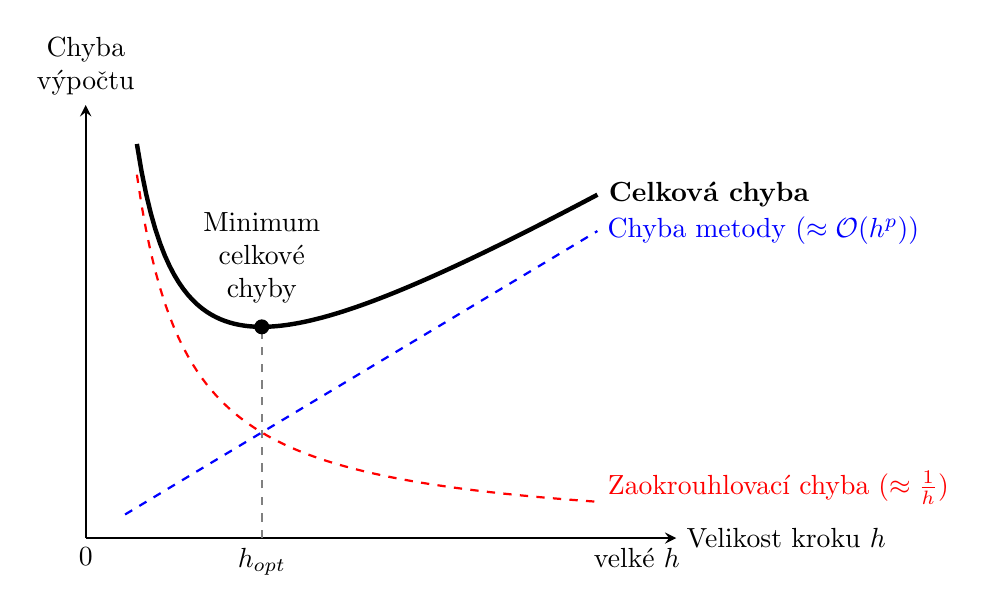
\begin{tikzpicture}[>=stealth]
        % Osy
        \draw[->, thick] (0,0) -- (7.5,0) node[right, align=center] {Velikost kroku $h$};
        \draw[->, thick] (0,0) -- (0,5.5) node[above, align=center] {Chyba\\výpočtu};
        
        % Osa logaritmická - naznačení směru k nule
        \node[below] at (0,0) {$0$};
        \node[below] at (7,0) {velké $h$};
        
        % Chyba metody (analytická chyba) - roste s rostoucím h
        % Vykreslíme jako lineární/polynomiální funkci (např. y = 0.6 * x)
        \draw[domain=0.5:6.5, color=blue, thick, dashed, samples=100] 
            plot (\x, {0.6*\x}) node[right] {\textcolor{blue}{Chyba metody ($\approx \mathcal{O}(h^p)$)}};
            
        % Zaokrouhlovací chyba (numerická chyba) - roste s klesajícím h
        % Vykreslíme jako nepřímou úměru (např. y = 3 / x)
        \draw[domain=0.65:6.5, color=red, thick, dashed, samples=100] 
            plot (\x, {3/\x}) node[right, yshift=5pt] {\textcolor{red}{Zaokrouhlovací chyba ($\approx \frac{1}{h}$)}};
            
        % Celková chyba = Chyba metody + Zaokrouhlovací chyba
        \draw[domain=0.65:6.5, color=black, ultra thick, samples=100] 
            plot (\x, {0.6*\x + 3/\x}) node[right, font=\bfseries] {Celková chyba};
            
        % Nalezení minima (optimálního h)
        % Minimum funkce f(x) = 0.6x + 3/x je v bodě x = sqrt(3/0.6) = sqrt(5) ≈ 2.236
        % y = 0.6*2.236 + 3/2.236 = 1.341 + 1.341 = 2.683
        \coordinate (Opt) at (2.236, 2.683);
        
        % Vyznačení optimálního bodu
        \draw[dashed, gray, thick] (2.236, 0) -- (Opt);
        \filldraw[black] (Opt) circle (2.5pt) node[above=5pt, align=center] {Minimum\\celkové\\chyby};
        \node[below, font=\bfseries] at (2.236, 0) {$h_{opt}$};
        
    \end{tikzpicture}
    \caption{Závislost celkové chyby numerického derivování na velikosti kroku $h$. Při příliš malém kroku dominuje zaokrouhlovací chyba počítače (červená křivka), při příliš velkém kroku je metoda matematicky nepřesná (modrá křivka). Naším cílem je najít optimální krok $h_{opt}$.}
    \label{fig:optimalni_h}
\end{figure}

\paragraph*{Zpřesnění výpočtu: Richardsonova extrapolace}
Vzhledem k nemožnosti libovolně zmenšovat krok $h$ se pro dosažení vysoké přesnosti využívá \textbf{Richardsonova extrapolace}.

\subsection{Numerické integrování}
Numerické integrování se používá k výpočtu určitého integrálu $\int_a^b f(x) dx$, pokud analytický výpočet neexistuje, je příliš složitý, nebo známe-li funkci pouze v diskrétních bodech.

\paragraph*{Princip:}
Základní myšlenka spočívá v nahrazení složité funkce $f(x)$ interpolačním polynomem, který lze snadno zintegrovat analyticky (tzv. Newton-Cotesovy vzorce).
\begin{itemize}
    \item \textbf{Základní formule:} Aplikují aproximaci polynomu rovnou na celý interval $[a, b]$. Jsou velmi nepřesné pro široké intervaly.
    \item \textbf{Složené formule:} Interval $[a, b]$ se rozdělí na $n$ stejných podintervalů o šířce $h = \frac{b-a}{n}$. Základní formule se aplikuje na každý podinterval zvlášť a výsledky se sečtou. Zvyšováním počtu dělení $n$ (zmenšováním $h$) dosahujeme vysoké přesnosti.
\end{itemize}

\paragraph*{Tři hlavní metody (Složené verze):}

\begin{enumerate}
    \item \textbf{Obdélníková metoda (Středová)}
    \begin{itemize}
        \item \textit{Princip:} Funkci na podintervalu nahradíme konstantou (polynom 0. stupně), konkrétně hodnotou funkce \textbf{v jeho středu}. Plocha je aproximována obdélníky.
        \item \textit{Vzorec:} $I \approx h \sum_{i=0}^{n-1} f(x_{i}+\frac{h}{2})$
        \item \textit{Chyba:} $|E_M(f,h)| \leq \frac{b-a}{24}M_2h^2$ ($\mathcal{O}(h^2)$)
    \end{itemize}
    
    \item \textbf{Lichoběžníková metoda}
    \begin{itemize}
        \item \textit{Princip:} Body funkce spojíme úsečkami (polynom 1. stupně). Původní plocha je nahrazena součtem ploch jednotlivých lichoběžníků.
        \item \textit{Vzorec:} Krajní body se započítají jednou, všechny vnitřní body dvakrát:
        \[ I \approx h \left( \frac{f(x_0)}{2} + \sum_{i=1}^{n-1} f(x_i) + \frac{f(x_n)}{2} \right) \]
        \item \textit{Chyba:}  $|E_T(f,h)| \leq \frac{b-a}{12}M_2h^2$ ($\mathcal{O}(h^2)$)
    \end{itemize}

    \item \textbf{Simpsonova metoda}
    \begin{itemize}
        \item \textit{Princip:} Funkci nahrazujeme po částech \textbf{parabolami} (polynom 2. stupně). Každá parabola je proložena přes 3 sousední body, proto metoda \textbf{vyžaduje sudý počet podintervalů}~$n$.
        \item \textit{Vzorec:} Střídají se váhy 4 (pro liché body) a 2 (pro sudé body):
        \[ I \approx \frac{h}{3} \left( f(x_0) + 2\sum_{i=1}^{n/2-1} f(x_{2i}) + 4\sum_{i=1}^{n/2} f(x_{2i-1}) + f(x_n) \right) \]
        \item \textit{Chyba:} $|E_S(f,h)| \leq \frac{b-a}{180}M_4h^4$ ($\mathcal{O}(h^4)$)
    \end{itemize}
\end{enumerate}

\begin{figure}[H]
    \centering
    
    % 1. STŘEDOVÁ OBDÉLNÍKOVÁ METODA
    \begin{minipage}{0.32\textwidth}
        \centering
        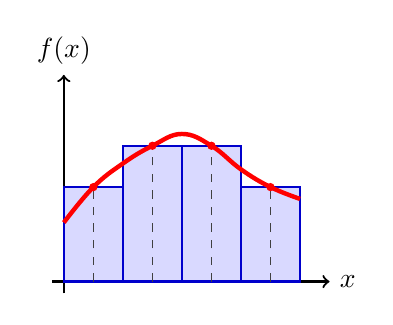
\begin{tikzpicture}[scale=0.75]
            % Osy
            \draw[->, thick] (-0.2, 0) -- (4.5, 0) node[right] {$x$};
            \draw[->, thick] (0, -0.2) -- (0, 3.5) node[above] {$f(x)$};
            
            % Obdélníky (výška určena středem intervalu)
            % Středy: 0.5 (y=1.6), 1.5 (y=2.3), 2.5 (y=2.3), 3.5 (y=1.6)
            \filldraw[fill=blue!15, draw=blue!80!black, thick] (0, 0) rectangle (1, 1.6);
            \filldraw[fill=blue!15, draw=blue!80!black, thick] (1, 0) rectangle (2, 2.3);
            \filldraw[fill=blue!15, draw=blue!80!black, thick] (2, 0) rectangle (3, 2.3);
            \filldraw[fill=blue!15, draw=blue!80!black, thick] (3, 0) rectangle (4, 1.6);
            
            % Vyznačení středů
            \foreach \x/\y in {0.5/1.6, 1.5/2.3, 2.5/2.3, 3.5/1.6} {
                \draw[dashed, darkgray] (\x, 0) -- (\x, \y);
                \fill[red] (\x, \y) circle (2pt);
            }
            
            % Samotná spojitá funkce
            \draw[ultra thick, red] plot [smooth, tension=0.7] coordinates { 
                (0,1) (0.5,1.6) (1,2) (1.5,2.3) (2,2.5) (2.5,2.3) (3,1.9) (3.5,1.6) (4,1.4) 
            };
        \end{tikzpicture}
        \caption*{Obdélníková (středová)}
    \end{minipage}\hfill
    %
    % 2. LICHOBĚŽNÍKOVÁ METODA
    \begin{minipage}{0.32\textwidth}
        \centering
        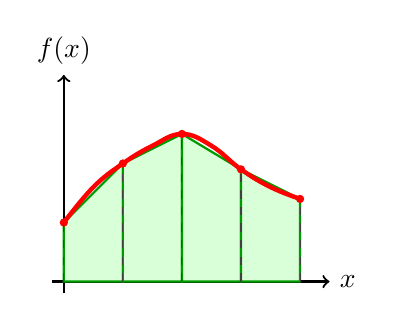
\begin{tikzpicture}[scale=0.75]
            % Osy
            \draw[->, thick] (-0.2, 0) -- (4.5, 0) node[right] {$x$};
            \draw[->, thick] (0, -0.2) -- (0, 3.5) node[above] {$f(x)$};
            
            % Lichoběžníky
            \filldraw[fill=green!15, draw=green!60!black, thick] (0,0) -- (0,1) -- (1,2) -- (1,0) -- cycle;
            \filldraw[fill=green!15, draw=green!60!black, thick] (1,0) -- (1,2) -- (2,2.5) -- (2,0) -- cycle;
            \filldraw[fill=green!15, draw=green!60!black, thick] (2,0) -- (2,2.5) -- (3,1.9) -- (3,0) -- cycle;
            \filldraw[fill=green!15, draw=green!60!black, thick] (3,0) -- (3,1.9) -- (4,1.4) -- (4,0) -- cycle;
            
            % Vyznačení uzlů
            \foreach \x/\y in {0/1, 1/2, 2/2.5, 3/1.9, 4/1.4} {
                \fill[red] (\x, \y) circle (2pt);
                \draw[dashed, darkgray] (\x, 0) -- (\x, \y);
            }
            
            % Samotná spojitá funkce
            \draw[ultra thick, red] plot [smooth, tension=0.7] coordinates { 
                (0,1) (0.5,1.6) (1,2) (1.5,2.3) (2,2.5) (2.5,2.3) (3,1.9) (3.5,1.6) (4,1.4) 
            };
        \end{tikzpicture}
        \caption*{Lichoběžníková}
    \end{minipage}\hfill
    %
    % 3. SIMPSONOVA METODA
    \begin{minipage}{0.32\textwidth}
        \centering
        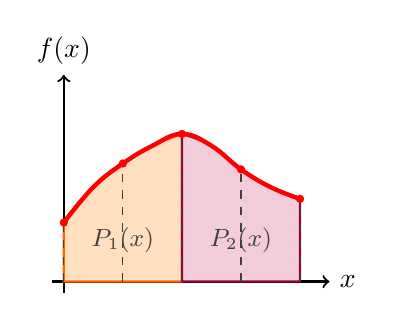
\begin{tikzpicture}[scale=0.75]
            % Osy
            \draw[->, thick] (-0.2, 0) -- (4.5, 0) node[right] {$x$};
            \draw[->, thick] (0, -0.2) -- (0, 3.5) node[above] {$f(x)$};
            
            % Simpson - první parabola (přes body 0, 1, 2)
            \fill[orange!25, draw=orange!80!red, thick] 
                (0,0) -- plot [smooth, tension=0.7] coordinates {(0,1) (0.5,1.6) (1,2) (1.5,2.3) (2,2.5)} -- (2,0) -- cycle;
            
            % Simpson - druhá parabola (přes body 2, 3, 4)
            \fill[purple!20, draw=purple!80!black, thick] 
                (2,0) -- plot [smooth, tension=0.7] coordinates {(2,2.5) (2.5,2.3) (3,1.9) (3.5,1.6) (4,1.4)} -- (4,0) -- cycle;
                
            % Svislé dělící čáry a uzly
            \foreach \x/\y in {0/1, 1/2, 2/2.5, 3/1.9, 4/1.4} {
                \draw[dashed, darkgray] (\x, 0) -- (\x, \y);
                \fill[red] (\x, \y) circle (2pt);
            }
            
            % Značky P1 a P2 pro paraboly
            \node[font=\small\bfseries, darkgray] at (1, 0.7) {$P_1(x)$};
            \node[font=\small\bfseries, darkgray] at (3, 0.7) {$P_2(x)$};
            
            % Samotná spojitá funkce
            \draw[ultra thick, red] plot [smooth, tension=0.7] coordinates { 
                (0,1) (0.5,1.6) (1,2) (1.5,2.3) (2,2.5) (2.5,2.3) (3,1.9) (3.5,1.6) (4,1.4) 
            };
        \end{tikzpicture}
        \caption*{Simpsonova (paraboly)}
    \end{minipage}
    
    \caption{Geometrická interpretace tří základních složených kvadraturních vzorců pro krok $h=1$. Červená křivka reprezentuje přesnou funkci $f(x)$. Obdélníková metoda využívá funkční hodnotu uprostřed podintervalu. Lichoběžníková metoda spojuje hranice úsečkou. Simpsonova metoda prokládá vždy trojicí bodů (dvěma podintervaly) parabolu ($P_1, P_2$).}
    \label{fig:integrace}
\end{figure}

\paragraph*{Zlepšení výsledků:}
\begin{itemize}
    \item Rekurzivní výpočet pro dvojnásobný počet bodů
    \item Rombergova metoda
\end{itemize} 

\paragraph*{Chyba výpočtu a stabilita:}
Na rozdíl od numerického derivování je numerické integrování \textbf{vysoce stabilní proces}. Integrál je ze své podstaty suma (součet ploch), takže náhodné zaokrouhlovací chyby (nebo šum v měřených datech) se často navzájem vyruší (vyhladí).

Protože analytický výpočet chyby závisí na derivacích integrované funkce (které většinou neznáme), používá se v praxi pro odhad chyby tzv. \textbf{Rungeho princip polovičního kroku}:
\begin{enumerate}
    \item Spočítáme integrál s krokem $h$ (označme $I_h$).
    \item Spočítáme integrál s polovičním krokem $h/2$ (označme $I_{h/2}$).
    \item Pokud je rozdíl $|I_{h} - I_{h/2}|$ menší než naše požadovaná přesnost $\varepsilon$, výpočet ukončíme a prohlásíme výsledek za dostatečně přesný. Pokud ne, krok znovu rozpůlíme.
\end{enumerate}

\newpage

\section{Numerické řešení soustav lineárních algebraických rovnic - přímé a nepřímé metody.}
\begin{quote}
    \textbf{Lineární algebraická rovnice a jejich soustavy, matice soustavy, Gaussova eliminační metoda, výběr hlavního prvku, vliv zaokrouhlovacích chyb, podmíněnost úlohy, LU rozklad matice, výpočet inverzní matice, výpočet determinantu. Iterační metody a kritéria jejich konvergence.}
\end{quote}

\subsection{Lineární algebraická rovnice a jejich soustavy}
Rovnice, ve které se neznámé vyskytují pouze v 1. mocnině a nejsou mezi sebou násobeny.
Soustava lineárních rovnic obsahuje více rovnic, které sdílí stejné neznámé.
\paragraph*{Základní pojmy a maticový zápis:}
Soustava $m$ lineárních algebraických rovnic o $n$ neznámých $x_1, x_2, \dots, x_n$ má obecný tvar:
\begin{align*}
    a_{11}x_1 + a_{12}x_2 + \dots + a_{1n}x_n &= b_1 \\
    a_{21}x_1 + a_{22}x_2 + \dots + a_{2n}x_n &= b_2 \\
    &\vdots \\
    a_{m1}x_1 + a_{m2}x_2 + \dots + a_{mn}x_n &= b_m
\end{align*}
Tento rozsáhlý zápis se v lineární algebře zkracuje do \textbf{maticového tvaru}:
\[ A \vec{x} = \vec{b} \]
kde definujeme následující prvky:
\begin{itemize}
    \item $A \in \mathbb{R}^{m \times n}$ je \textbf{matice soustavy} tvořená koeficienty $a_{ij}$.
    \item $\vec{x} \in \mathbb{R}^n$ je \textbf{vektor neznámých} (sloupcový vektor).
    \item $\vec{b} \in \mathbb{R}^m$ je \textbf{vektor pravých stran} (absolutní členy).
\end{itemize}
Spojením matice $A$ a vektoru $\vec{b}$ vzniká tzv. \textbf{rozšířená matice soustavy} $[A | \vec{b}]$, se kterou pracují základní vyhodnocovací a řešicí algoritmy.

\paragraph*{Řešitelnost soustavy (Frobeniova věta):}
Z čistě algebraického hlediska rozhoduje o existenci řešení \textbf{Frobeniova věta}. Zkoumáme hodnost matice $h(A)$ (počet jejích lineárně nezávislých řádků):
\begin{enumerate}
    \item \textbf{Nemá řešení:} Pokud se hodnost matice soustavy liší od hodnosti rozšířené matice ($h(A) \neq h(A|\vec{b})$). Soustava obsahuje spor.
    \item \textbf{Má právě 1 řešení:} Pokud se hodnosti rovnají a jsou rovny počtu neznámých ($h(A) = h(A|\vec{b}) = n$). Matice $A$ je v tomto případě \textbf{regulární} (je čtvercová a její determinant je nenulový, $\det(A) \neq 0$).
    \item \textbf{Má nekonečně mnoho řešení:} Pokud se hodnosti rovnají, ale jsou menší než počet neznámých ($h(A) = h(A|\vec{b}) < n$). Řešení pak závisí na $(n - h)$ volných parametrech.
\end{enumerate}

\begin{quote}
\textbf{Poznámka k hodnosti matice ($h(A)$):} 
Hodnost matice udává maximální počet jejích \textbf{lineárně nezávislých} řádků (nebo sloupců). 
Pokud má čtvercová matice o rozměrech $n \times n$ hodnost přesně $n$, říkáme, že má \textbf{plnou hodnost}. Taková matice je regulární a má nenulový determinant.
\end{quote}

\subsection{Gaussova eliminační metoda}

Gaussova eliminační metoda (GEM) patří mezi přímé metody řešení soustav lineárních algebraických rovnic. Cílem je nalézt vektor řešení $\vec{x} \in \mathbb{R}^n$ splňující rovnici
\[ A \vec{x} = \vec{b} \]
kde $A \in \mathbb{R}^{n \times n}$ je regulární čtvercová matice soustavy a $\vec{b} \in \mathbb{R}^n$ je vektor pravé strany.

\subsubsection{Algoritmus Gaussovy eliminační metody}
Algoritmus GEM se skládá ze dvou základních, po sobě jdoucích fází:
\begin{enumerate}
    \item \textbf{Přímý chod (eliminace):} Rozšířená matice soustavy $[A|\vec{b}]$ je pomocí elementárních řádkových úprav (záměna řádků, přičtení lineární kombinace jiných řádků) postupně převedena na horní trojúhelníkový tvar $[U|\vec{c}]$, kde $U$ je horní trojúhelníková matice s nulovými prvky pod hlavní diagonálou. 
    
    \item \textbf{Zpětný chod (substituce):} Získaná soustava s horní trojúhelníkovou maticí $U\vec{x} = \vec{c}$ se řeší postupně od poslední neznámé po první zpětnou substitucí.
\end{enumerate}

\subsubsection{Výběr hlavního prvku (Pivoting)}
V počítačové aritmetice s omezenou přesností nastává problém tehdy, je-li právě řešený prvek na diagonále $\approx 0$. Dělení velmi malým číslem vede ke vzniku extrémně velkých multiplikátorů $m_{ik}$, což způsobuje šíření a zvětšování zaokrouhlovacích chyb v následujících úpravách matice. 
Tento jev se eliminuje \textit{výběrem hlavního prvku} (pivotingem):
\begin{itemize}
    \item \textbf{Částečný (sloupcový) výběr prvku:} V $k$-tém kroku hledáme v $k$-tém sloupci na diagonále a pod ní prvek s maximální absolutní hodnotou, tedy index $r$ takový, že:
    
    \[ |a_{rk}^{(k-1)}| = \max_{k \le i \le n} |a_{ik}^{(k-1)}|.\]
    
    Následně se prohodí celý $k$-tý řádek s řádkem $r$. Tím je zaručeno, že pro všechny multiplikátory platí $|m_{ik}| \le 1$, což stabilizuje výpočet.
    Tedy vybereme z aktuálního sloupce největší číslo (podle absolutní hodnoty) a vyměníme řádky, aby to číslo bylo nahoře = hlavní prvek.
    \item \textbf{Úplný výběr prvku:} Maximum se hledá v celé zbývající podmatici o rozměrech $(n-k+1) \times (n-k+1)$. Tento postup vyžaduje jak prohození řádků, tak prohození sloupců (což znamená přeuspořádání složek vektoru neznámých $\vec{x}$). Úplný výběr je numericky nejstabilnější, ale kvůli vysoké vyhledávací náročnosti se v praxi využívá zřídka. Částečný výběr obvykle poskytuje dostatečnou přesnost.
\end{itemize}

\subsubsection{Vliv zaokrouhlovacích chyb}
Každá aritmetická operace zavádí drobnou relativní chybu. U rozsáhlých soustav rovnic dochází ke kumulaci těchto chyb.
Hlavním rizikem v GEM je tzv. \textit{odčítání blízkych čísel} (cancellation) a následné násobení velkými čísly. Pokud není implementován výběr hlavního prvku, mohou chyby zcela znehodnotit výsledek, což znamená, že algoritmus je \textit{numericky nestabilní}. Použitím částečného pivotingu se GEM stává zpětně stabilním algoritmem.

\subsubsection{Podmíněnost úlohy}
Mírou této podmíněnosti GEM je \textbf{číslo podmíněnosti matice} $\kappa(A)$, definované vzhledem k přidružené maticové normě. Číslo podmíněnosti se vypočítá jako součin normy matice a normy její inverzní matice:
\[ 
\kappa(A) = \|A\| \cdot \|A^{-1}\|.
\]
Pro libovolnou matici platí $\kappa(A) \ge 1$. Podle velikosti tohoto čísla rozlišujeme úlohy na:
\begin{itemize}
    \item \textbf{Dobře podmíněné ($\kappa(A) \approx 1$):} Malé relativní změny na vstupu vyvolají adekvátně malé relativní změny v řešení.
    \item \textbf{Špatně podmíněné ($\kappa(A) \gg 1$):} I nepatrná chyba ve vstupních datech (např. zaokrouhlení při zadávání koeficientů) může způsobit obrovské, řádové změny ve výsledném vektoru $\vec{x}$. Matice s extrémně vysokým číslem podmíněnosti se blíží maticím singulárním.
\end{itemize}
Je-li matice soustavy špatně podmíněná, žádný numericky stabilní algoritmus (včetně GEM s úplným výběrem prvků) nedokáže zajistit přesné řešení, neboť velká chyba výstupu je přirozeným důsledkem vlastností zadání úlohy.

\subsection{LU rozklad matice}

LU rozklad je přímá metoda řešení soustavy $A\vec{x} = \vec{b}$, která spočívá v rozkladu regulární čtvercové matice $A$ na součin dvou trojúhelníkových matic:
\[ 
A = LU,
\]
kde $L$ je dolní (\textit{Lower}) trojúhelníková matice s jednotkami na hlavní diagonále a $U$ je horní (\textit{Upper}) trojúhelníková matice, která odpovídá výsledku matice $A$ po přímém chodu Gaussovy eliminace.

\subsubsection{Postup řešení}
Jakmile je znám rozklad $A = LU$, původní soustava $LU\vec{x} = \vec{b}$ se řeší ve dvou krocích:
\begin{enumerate}
    \item \textbf{Dopředná substituce:} Řešíme soustavu $L\vec{y} = \vec{b}$ pro pomocný vektor $\vec{y}$.
    \item \textbf{Zpětná substituce:} Řešíme soustavu $U\vec{x} = \vec{y}$ pro cílový vektor řešení $\vec{x}$.
\end{enumerate}

\subsubsection{Výhody a složitost}
\begin{itemize}
    \item \textbf{Efektivita:} LU rozklad je výhodný zejména v případech, kdy řešíme více soustav se stejnou maticí $A$, ale různými pravými stranami $\vec{b}$. Rozklad se provede pouze jednou a pro každou novou pravou stranu se provádí pouze substituce.
    \item \textbf{Vztah k determinantu:} Determinant matice lze po rozkladu snadno spočítat jako součin diagonálních prvků matice $U$, tedy $\det(A) = \prod_{i=1}^n u_{ii}$.
\end{itemize}

\subsection{Výpočet inverzní matice}

Inverzní matice $A^{-1}$ k regulární čtvercové matici $A$ řádu $n$ je definována vztahem 
\[
A A^{-1} = I,
\]
kde $I$ je jednotková matice řádu $n$.
Inverzní matice existuje, jen pokud $\det(A) \neq 0$.
Pro praktický výpočet se využívají dva hlavní přístupy:
\begin{itemize}
    \item \textbf{Využití LU rozkladu:} Matice $A$ se pouze jednou rozloží na $PA = LU$. Následně se pro každý z $n$ sloupců $\vec{e}_i$ provede rychlá dopředná a zpětná substituce.
    \item \textbf{Gaussova-Jordanova eliminace:} Rozšířená matice tvaru $[A \,|\, I]$ se pomocí ekvivalentních řádkových úprav převede přímo na redukovaný schodovitý tvar. Z levé poloviny se stane jednotková matice a v pravé polovině vznikne hledaná matice inverzní: $[A \,|\, I] \sim [I \,|\, A^{-1}]$.
\end{itemize}

\subsection{Výpočet determinantu}

Výpočet determinantu $\det(A)$ podle definice nebo pomocí Laplaceova rozvoje je výpočetně neúnosný pro matice větších řádů, neboť vyžaduje asymptoticky $\mathcal{O}(n!)$ operací. V numerické matematice se proto determinant počítá výhradně pomocí Gaussovy eliminace nebo LU rozkladu, což redukuje složitost na $\mathcal{O}(n^3)$.

Z vlastností determinantu plyne, že determinant horní i dolní trojúhelníkové matice je roven součinu prvků na její hlavní diagonále. Máme-li k dispozici LU rozklad s částečným výběrem prvku $PA = LU$, platí podle Cauchyovy věty o determinantu součinu:
\[
\det(P) \cdot \det(A) = \det(L) \cdot \det(U).
\]

Z vlastností jednotlivých matic rozkladu odvodíme:
\begin{itemize}
    \item Matice $L$ má na diagonále pouze jedničky, tedy $\det(L) = 1$.
    \item Matice $U$ je horní trojúhelníková, její determinant je součin diagonálních prvků $u_{ii}$.
    \item Permutační matice $P$ vznikla výměnou řádků. Každá výměna řádků mění znaménko determinantu. Proto platí $\det(P) = (-1)^s$, kde $s$ je celkový počet výměn řádků provedených během eliminace.
\end{itemize}

Výsledný vzorec pro efektivní výpočet determinantu je tedy dán jako:
\[
\det(A) = (-1)^s \prod_{i=1}^n u_{ii} = (-1)^s \cdot u_{11} \cdot u_{22} \cdots u_{nn}.
\]
Pokud matice $A$ není regulární, na diagonále matice $U$ se objeví alespoň jedna nula a součin automaticky vyjde nulový, což správně odpovídá singulární matici.

\paragraph*{Sarrusovo pravidlo}

Zatímco pro velké matice se využívá výhradně Gaussova eliminace nebo LU rozklad, pro ruční výpočet determinantu malých matic řádu $n=3$ se často používá přímý vzorec známý jako \textbf{Sarrusovo pravidlo}. 

Pro matici $A \in \mathbb{R}^{3 \times 3}$ ve tvaru:
\[
A = \begin{pmatrix}
a_{11} & a_{12} & a_{13} \\
a_{21} & a_{22} & a_{23} \\
a_{31} & a_{32} & a_{33}
\end{pmatrix}
\]
je Sarrusovo pravidlo mnemotechnickou pomůckou. Vypočte se jako součet součinů tří prvků ve směru hlavní diagonály (zleva nahoře doprava dolů), od kterého se odečte součet součinů tří prvků ve směru vedlejší diagonály (zprava nahoře doleva dolů):
\[
\begin{split}
\det(A) = {} & a_{11}a_{22}a_{33} + a_{12}a_{23}a_{31} + a_{13}a_{21}a_{32} \\
             & - (a_{13}a_{22}a_{31} + a_{11}a_{23}a_{32} + a_{12}a_{21}a_{33}).
\end{split}
\]

\subsection{Iterační metody a kritéria jejich konvergence}

Na rozdíl od přímých metod (jako GEM či LU rozklad), které naleznou přesné řešení v konečném počtu kroků, generují iterační metody posloupnost aproximací $\vec{x}^{(0)}, \vec{x}^{(1)}, \dots, \vec{x}^{(k)}$, která konverguje k přesnému řešení $\vec{x}$. Tyto metody se využívají především pro řešení obrovských a řídkých soustav, u kterých by přímé metody byly příliš paměťově a časově náročné.

Obecný tvar lineární iterační metody pro řešení soustavy $A\vec{x} = \vec{b}$ je:
\[
\vec{x}^{(k+1)} = T\vec{x}^{(k)} + \vec{c},
\]
kde $T$ je tzv. iterační matice a $\vec{c}$ je konstantní vektor. 

\subsubsection{Kritéria konvergence}
Jakobiho i Gauss-Seidelova metoda konvergují, pokud matice soustavy $A$ je:
\begin{itemize}
    \item \textbf{Ryze řádkově (či sloupcově) diagonálně dominantní}: Absolutní hodnota prvku na diagonále je větší než součet absolutních hodnot ostatních prvků v daném řádku (resp. sloupci).
    \item Gauss-Seidelova metoda konverguje navíc i tehdy, pokud je matice $A$ \textbf{symetrická a pozitivně definitní}.
\end{itemize}
    \begin{quote}
        \textbf{Pozitivní definitnost:} 
        Symetrická matice $A$ řádu $n$ je podle Sylvesterova kritéria pozitivně definitní právě tehdy, když jsou všechny její vedoucí hlavní minory (determinanty levých horních podmatic) ostře kladné.
        Základní vlastností pozitivně definitní matice, že všechna její vlastní čísla jsou kladná.
    \end{quote}

\subsubsection{Jakobiho metoda}
Matice soustavy se rozloží na tvar $A = D + L + U$, kde $D$ je diagonální matice a $L, U$ jsou ostře dolní a horní trojúhelníkové matice (mají na diagonále nuly). Iterační předpis je odvozen ze vztahu $D\vec{x} = \vec{b} - (L+U)\vec{x}$ a zní:
\[
\vec{x}^{(k+1)} = D^{-1}(\vec{b} - (L+U)\vec{x}^{(k)}).
\]
Po složkách to znamená, že nová aproximace $i$-té složky se počítá \textbf{výhradně z hodnot předchozího kroku} $k$. Matice $D$ musí mít nenulové diagonální prvky.

\subsubsection{Gauss-Seidelova metoda}
Jedná se o vylepšení Jakobiho metody. Při výpočtu $i$-té složky vektoru $\vec{x}^{(k+1)}$ se okamžitě využijí již vypočtené novější hodnoty složek s indexy $1$ až $i-1$. Iterační předpis v maticovém tvaru je:
\[
\vec{x}^{(k+1)} = (D+L)^{-1}(\vec{b} - U\vec{x}^{(k)}).
\]
Díky průběžnému využívání zpřesněných hodnot konverguje Gauss-Seidelova metoda obvykle rychleji než Jakobiho metoda.

\subsubsection{Ritzova iterační metoda}
Tato metoda se principiálně liší od předchozích a vychází z \textbf{variačního počtu}. Je určena pro soustavy, kde matice $A$ je symetrická a pozitivně definitní. 

\section{Popis datového souboru}
\begin{quote}
    \textbf{Typy dat a měrné stupnice. Charakteristika polohy (střední hodnota, modus, medián), variability (směrodatná odchylka, rozptyl), relativní četnosti. Rozdělení hodnot (kvantily, kumulativní relativní četnosti). Vizualizace (histogram, sloupcový, kruhový a krabicový graf). Specifika popisu dat nenumerických.}
\end{quote}

\subsection{Typy dat a měrné stupnice}
\paragraph*{Typy dat (Základní rozdělení):}
Data obecně dělíme do dvou hlavních skupin:
\begin{itemize}
    \item \textbf{Kvalitativní (Kategoriální) data:} Popisují vlastnosti, stavy nebo kategorie. I když jsou někdy kódována čísly (např. $1 = \text{žena}$, $2 = \text{muž}$), nemají matematický význam (nelze je sčítat, porovnávat, atd.).
    \item \textbf{Kvantitativní (Numerická) data:} Vyjadřují množství nebo velikost a lze s nimi provádět matematické operace. Dělí se dále na:
    \begin{itemize}
        \item \textit{Diskrétní:} Nabývají pouze oddělených, většinou celočíselných hodnot (např. počet dětí v rodině, počet defektů na výrobku). Vznikají počítáním.
        \item \textit{Spojitá:} Mohou nabývat libovolné reálné hodnoty v určitém intervalu (např. výška, hmotnost, čas). Vznikají měřením.
    \end{itemize}
\end{itemize}

\paragraph*{Měrné stupnice:}
Podle toho, jaké matematické operace s hodnotami dávají logický smysl, rozdělujeme data do čtyř měrných stupnic (od nejchudší po nejbohatší):

\begin{enumerate}
    \item \textbf{Nominální stupnice:}
    \begin{itemize}
        \item \textit{Charakteristika:} Pouze pojmenovává kategorie. Neexistuje mezi nimi žádné logické pořadí.
        \item \textit{Operace:} Lze testovat pouze rovnost ($=$ a $\neq$).
        \item \textit{Příklady:} Barva očí, krevní skupina, rodné číslo, PSČ.
    \end{itemize}
    
    \item \textbf{Ordinální stupnice:}
    \begin{itemize}
        \item \textit{Charakteristika:} Kategorie lze logicky seřadit (víme, co je "víc" a "míň"), ale neznáme přesnou vzdálenost mezi nimi.
        \item \textit{Operace:} Lze navíc porovnávat velikost ($<, >$).
        \item \textit{Příklady:} Stupeň vzdělání (ZŠ, SŠ, VŠ), vojenské hodnosti, hodnocení spokojenosti (1 až 5 hvězdiček).
    \end{itemize}
    
    \item \textbf{Intervalová stupnice:}
    \begin{itemize}
        \item \textit{Charakteristika:} Hodnoty lze seřadit a víme, o kolik se liší (intervaly jsou stejně velké). Chybí zde však absolutní nula (nula je jen dohodnutý bod, neznamená "nic").
        \item \textit{Operace:} Lze sčítat a odčítat ($+, -$). Nelze dělit (nemá smysl počítat násobky).
        \item \textit{Příklady:} Teplota ve stupních Celsia (20°C není dvakrát teplejší než 10°C), kalendářní roky.
    \end{itemize}
    
    \item \textbf{Poměrová stupnice:}
    \begin{itemize}
        \item \textit{Charakteristika:} Má všechny vlastnosti intervalové stupnice a navíc má přirozenou (absolutní) nulu, která znamená úplnou absenci měřené vlastnosti.
        \item \textit{Operace:} Lze provádět všechny matematické operace včetně násobení a dělení ($\cdot, /$).
        \item \textit{Příklady:} Věk, mzda, hmotnost, délka (10 metrů je přesně dvakrát delší než 5 metrů).
    \end{itemize}
\end{enumerate}

\subsection{Charakteristiky polohy}
Ukazují, kolem jaké hodnoty se data koncentrují (tzv. míry střední tendence).

\begin{itemize}
    \item \textbf{Střední hodnota (Aritmetický průměr, $\bar{x}$ nebo $\mu$ (mý)):} 
    Součet všech hodnot vydělený jejich počtem.
    \begin{itemize}
        \item \textit{Výhoda:} Využívá všechny hodnoty v souboru.
        \item \textit{Nevýhoda:} Je extrémně citlivý na odlehlé hodnoty. Jeden miliardář v místnosti drasticky zkreslí průměrný plat všech přítomných.
    \end{itemize}
    
    \item \textbf{Medián ($\tilde{x}$):} 
    Prostřední hodnota v seřazeném souboru dat (50 \% hodnot je menších, 50 \% větších).
    \begin{itemize}
        \item \textit{Výhoda:} Je robustní vůči odlehlým hodnotám. Používá se typicky pro platy nebo ceny nemovitostí, kde průměr dává zkreslený obraz.
    \end{itemize}
    
    \item \textbf{Modus ($\hat{x}$):} 
    Nejčastěji se vyskytující hodnota v souboru.
    \begin{itemize}
        \item \textit{Výhoda:} Jako jediná míra polohy se dá použít i pro nominální data (např. nejčastější barva očí, nejprodávanější značka auta).
    \end{itemize}
\end{itemize}

\subsection{Charakteristiky variability}
Určuje odchylky hodnot v datovém souboru (průměrná teplota v poušti může být příjemných 20°C, ale přes den je 50°C a v noci -10°C).

\begin{itemize}
    \item \textbf{Rozptyl ($s^2$ pro výběr, $\sigma^2$ (sigma) pro populaci):} 
    Průměr ze čtverců odchylek jednotlivých hodnot od aritmetického průměru.
    \begin{itemize}
        \item \textit{Populační rozptyl} (počítáme z úplně všech prvků, $N$ je velikost populace, $\mu$ je populační průměr):
        \[ \sigma^2 = \frac{1}{N} \sum_{i=1}^{N} (x_i - \mu)^2 \]
        \item \textit{Výběrový rozptyl} (počítáme jen ze vzorku, $n$ je velikost vzorku, $\bar{x}$ je výběrový průměr). Dělí se $n-1$ (tzv. Besselova korekce), aby byl odhad nezkreslený:
        \[ s^2 = \frac{1}{n-1} \sum_{i=1}^{n} (x_i - \bar{x})^2 \]
    \end{itemize}

    kde $(x_i - \bar{x})^2$ je čtverec vzdáleností bodů od průměru.
    
    \item \textbf{Směrodatná odchylka ($s$ nebo $\sigma$):} 
    Druhá odmocnina z rozptylu.
    \begin{itemize}
        \item \textit{Populační:} $\sigma = \sqrt{\sigma^2}$
        \item \textit{Výběrová:} $s = \sqrt{s^2}$
        \item \textit{Výhoda:} Vrací variabilitu zpět do původních jednotek (např. metry, koruny). Udává, o kolik se hodnoty typicky odchylují od průměru.
    \end{itemize}
\end{itemize}

\subsection{Absolutní a relativní četnost}
Používají se především pro kvalitativní a diskrétní data k popisu jejich rozložení.

\begin{itemize}
    \item \textbf{Absolutní četnost ($n_i$):} Udává, \textit{kolikrát} se daná varianta vyskytla v souboru (např. 15 studentů dostalo jedničku). Součet absolutních četností je roven celkovému rozsahu souboru $n$.
    \item \textbf{Relativní četnost ($p_i$):} Poměr absolutní četnosti k celkovému počtu měření ($p_i = \frac{n_i}{n}$). 
    Udává se jako desetinné číslo (od 0 do 1) nebo v procentech (např. 30 \% studentů).
    \begin{itemize}
        \item \textit{Využití:} Je nezbytná pro porovnávání různě velkých souborů (absolutní počty nelze srovnávat, pokud má jeden vzorek 100 lidí a druhý 1000 lidí).
    \end{itemize}
\end{itemize}

\subsection{Rozdělení hodnot}
\paragraph*{Kvantily}
Kvantil je hodnota, která rozděluje seřazený datový soubor na části v určitém procentuálním poměru. 
\begin{itemize}
    \item \textbf{Percentily ($P_k$):} Rozdělují data na 100 dílů (po 1 \%). Například $P_{90}$ (90. percentil) znamená, že 90 \% hodnot je menších (nebo rovných) a 10 \% hodnot je větších než tento bod.
    \item \textbf{Kvartily ($Q$):} Rozdělují data na 4 čtvrtiny (po 25 \%). Jsou nejpoužívanější:
    \begin{itemize}
        \item $Q_1$ (\textbf{Dolní kvartil}): 25 \% hodnot je pod ním.
        \item $Q_2$ (\textbf{Medián}): 50 \% hodnot je pod ním (střed).
        \item $Q_3$ (\textbf{Horní kvartil}): 75 \% hodnot je pod ním.
    \end{itemize}
\end{itemize}

\paragraph*{Kumulativní relativní četnosti}
Zatímco obyčejná relativní četnost říká, jaká část dat spadá do jedné konkrétní kategorie, kumulativní četnost hodnoty postupně sčítá (kumuluje).
\begin{itemize}
    \item \textbf{Význam:} Odpovídá na otázku: \textit{„Kolik procent dat je menších nebo rovných dané hodnotě?“}
    \item \textbf{Vlastnosti:} Začíná na 0 a s každou další hodnotou roste, až u maximální hodnoty v souboru dosáhne přesně 1 (neboli 100 \%).
\end{itemize}

\subsection{Vizualizace dat}
\paragraph*{1. Sloupcový graf (Bar chart)}
\begin{itemize}
\item \textbf{Použití:} Pro \textbf{kvalitativní (kategoriální)} nebo diskrétní data (např. barva očí, vzdělání).
\item \textbf{Vzhled:} Mezi sloupci jsou \textbf{viditelné mezery}, protože kategorie spolu číselně nesouvisejí.
\end{itemize}
\begin{figure}[h]
    \centering
    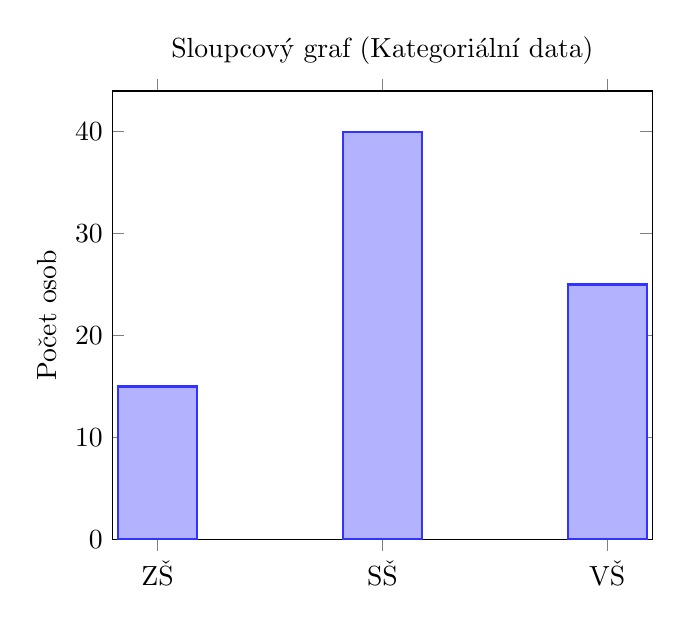
\begin{tikzpicture}
        \begin{axis}[
            ybar, % typ grafu: vertikální sloupce
            symbolic x coords={ZŠ, SŠ, VŠ},
            xtick=data,
            ymin=0,
            bar width=1cm,
            ylabel={Počet osob},
            title={Sloupcový graf (Kategoriální data)}
        ]
            \addplot[fill=blue!30, draw=blue!80, thick] coordinates {(ZŠ, 15) (SŠ, 40) (VŠ, 25)};
        \end{axis}
    \end{tikzpicture}
\end{figure}
\paragraph*{2. Histogram}
\begin{itemize}
\item \textbf{Použití:} Pro \textbf{spojitá kvantitativní data} (např. výška, hmotnost, čas).
\item \textbf{Vzhled:} Osa x představuje číselnou osu rozdělenou do intervalů. Sloupce na sebe těsně navazují (bez mezer), což znázorňuje spojitost dat.
\end{itemize}
\begin{figure}[H]
    \centering
    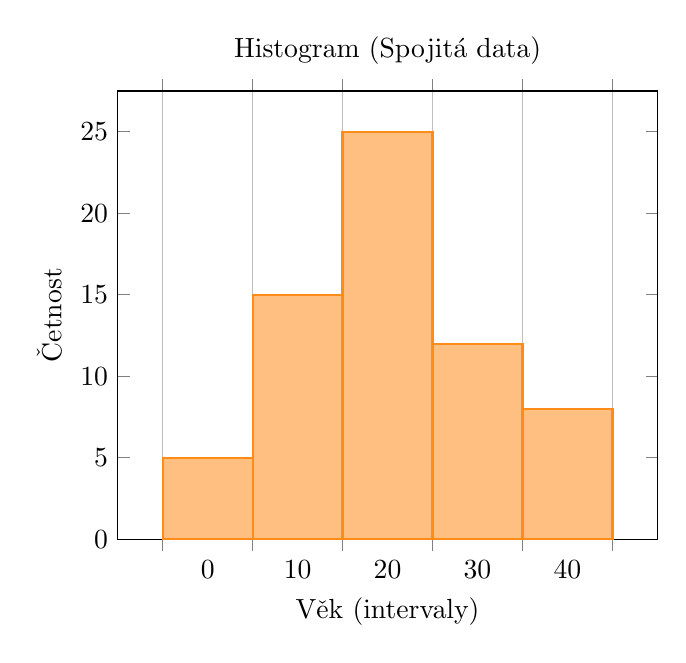
\begin{tikzpicture}
        \begin{axis}[
            ybar interval, % typ grafu: intervalový histogram
            xtick=data,
            ymin=0,
            ylabel={Četnost},
            xlabel={Věk (intervaly)},
            title={Histogram (Spojitá data)}
        ]
            % Souřadnice: (začátek intervalu, výška sloupce). Poslední bod určuje konec osy.
            \addplot[fill=orange!50, draw=orange!90, thick] coordinates {(0, 5) (10, 15) (20, 25) (30, 12) (40, 8) (50, 0)};
        \end{axis}
    \end{tikzpicture}
\end{figure}
\paragraph*{3. Kruhový graf (Pie chart)}
\begin{itemize}
\item \textbf{Použití:} Pro zobrazení \textbf{relativních četností (podílů z celku)}.
\item \textbf{Pravidlo:} Vhodný pouze pro malý počet kategorií (ideálně do 5). Všechny výseče musí dát dohromady 100 %.
\end{itemize}
\begin{figure}[H]
    \centering
    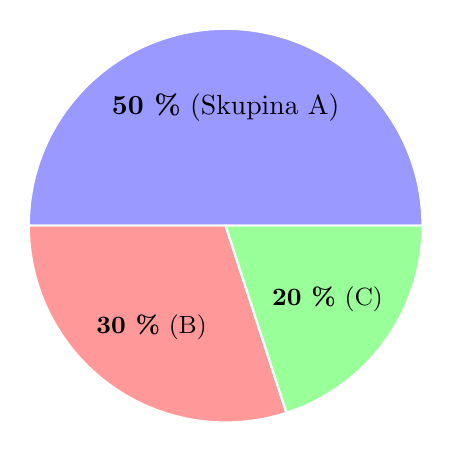
\begin{tikzpicture}
        % Kreslení kruhového grafu pomocí čistého TikZ (bez nutnosti dalších balíčků)
        % 50% = 180 stupňů, 30% = 108 stupňů, 20% = 72 stupňů
        \draw[fill=blue!40, thick, draw=white] (0,0) -- (0:2.5) arc (0:180:2.5) -- cycle;
        \node at (90:1.5) {\textbf{50 \%} (Skupina A)};
        
        \draw[fill=red!40, thick, draw=white] (0,0) -- (180:2.5) arc (180:288:2.5) -- cycle;
        \node[font=\small] at (234:1.6) {\textbf{30 \%} (B)};
        
        \draw[fill=green!40, thick, draw=white] (0,0) -- (288:2.5) arc (288:360:2.5) -- cycle;
        \node[font=\small] at (324:1.6) {\textbf{20 \%} (C)};
    \end{tikzpicture}
    \caption{Kruhový graf (Podíly z celku)}
\end{figure}
\paragraph*{4. Krabicový graf (Boxplot)}
\begin{itemize}
\item \textbf{Použití:} Ideální pro vizualizaci \textbf{kvartilů} a detekci \textbf{odlehlých hodnot}. Skvěle se hodí pro porovnávání více skupin dat vedle sebe.
\item \textbf{Vzhled:} Krabice vymezuje prostředních 50\% dat (od $Q_1$ do $Q_3$), čára uvnitř je medián. Hmatníky (ty věci nad a pod krabicí) sahají k minimu a maximu. Tečky mimo vousy jsou odlehlé hodnoty. (Občas je znažena i průměra hodnota.)
\end{itemize}
\begin{figure}[H]
    \centering
    \begin{tikzpicture}
        \begin{axis}[
            boxplot/draw direction=y, % horizontální boxplot
            xtick={1}, 
            xticklabels={Měření 1},
            ymin=0, ymax=25,
            title={Krabicový graf (Boxplot)}
        ]
            \addplot+[
                boxplot prepared={
                    lower whisker=4,  % Minimum (bez outlierů)
                    lower quartile=8, % Q1
                    median=12,        % Q2 (medián)
                    upper quartile=16,% Q3
                    upper whisker=21  % Maximum (bez outlierů)
                },
                mark=*, % značka pro outliery
                color=teal, solid, fill=teal!20, thick
            ] coordinates {(0, 1) (0, 24)}; % Souřadnice (y, hodnota outlieru)
        \end{axis}
    \end{tikzpicture}
\end{figure}

\subsection{Specifika popisu dat nenumerických}
Nenumerická (kvalitativní či kategoriální) data vyžadují specifický přístup, protože jejich hodnoty reprezentují vlastnosti, názvy nebo stavy, u kterých nelze provádět běžné aritmetické operace (nelze je sčítat, dělit, atd.).

\paragraph*{Omezení klasických popisných statistik:}
\begin{itemize}
    \item \textbf{Míry polohy:} Aritmetický průměr nelze použít vůbec. U nominálních dat lze určit pouze \textbf{modus} (nejčetnější kategorii). U ordinálních dat (kategorie lze logicky seřadit) má smysl hledat navíc i \textbf{medián} a \textbf{kvartily}.
    \item \textbf{Míry variability:} Klasický rozptyl či směrodatná odchylka nemají smysl. Variabilita se popisuje počtem unikátních kategorií a tím, jak rovnoměrně jsou mezi ně data rozdělena (zda převažuje jedna kategorie, nebo je datový soubor velmi heterogenní).
\end{itemize}

\paragraph*{Hlavní nástroje pro popis:}
\begin{itemize}
    \item \textbf{Tabulky četností:} Základem je vždy spočítání absolutních a relativních (procentuálních) četností jednotlivých kategorií.
    \item \textbf{Kontingenční tabulky:} Slouží ke zkoumání závislosti mezi dvěma kategoriálními proměnnými (např. vztah mezi stupněm vzdělání a místem bydliště). Ukazují četnosti průniků jednotlivých kategorií.
\end{itemize}

\section{Princip inference}
\begin{quote}
    \textbf{Populace, vzorek (výběr), bodový odhad parametru, výběrová chyba, zobecnění výsledku. Pro střední hodnotu a relativní četnost: směrodatná chyba a konstrukce intervalového odhadu. Statistické hypotézy o střední hodnotě a podílu (hypotézy, rozhodovací pravidla, chyba I. a II. druhu).}
\end{quote}

\subsection{Populace a vzorek}
\begin{itemize}
    \item \textbf{Populace:} Kompletní množina všech objektů, osob nebo jevů, o kterých chceme zjistit nějakou informaci (např. všichni oprávnění voliči v ČR, všechny vyrobené žárovky v továrně).
    \begin{itemize}
        \item Číselné charakteristiky celé populace nazýváme \textbf{parametry} (značíme řecky: $\mu$ (mý) pro průměr, $\sigma^2$ (sigma) pro rozptyl). V praxi jsou většinou neznámé.
    \end{itemize}
    \item \textbf{Vzorek / Výběr:} Část populace, kterou reálně změříme. 
    \begin{itemize}
        \item Číselné charakteristiky spočítané ze vzorku nazýváme \textbf{statistiky} (značíme latinkou: $\bar{x}$ pro průměr, $s^2$ pro rozptyl).
        \item \textbf{Reprezentativnost:} Aby mělo zkoumání vzorku smysl, musí vzorek věrně odrážet složení populace. Toho se nejlépe dosahuje prostým \textbf{náhodným výběrem}.
    \end{itemize}
\end{itemize}

\subsection{Bodový odhad parametru}
Bodový odhad znamená, že neznámý parametr populace (např. skutečný průměrný plat v ČR) je nahrazen jedním konkrétním číslem spočítaným ze vzorku (např. průměrný plat tisíce dotázaných lidí, tedy odhadem $\mu$ je $\bar{x}$).

Správný bodový odhad by měl splňovat dvě klíčové matematické vlastnosti:
\begin{itemize}
    \item \textbf{Nestrannost (Nevychýlenost):} Odhad systematicky nenadceňuje ani nepodceňuje skutečnost (očekávaná hodnota odhadu se rovná skutečnému parametru). \textit{Proto u výběrového rozptylu dělíme $n-1$, aby byl nestranný.}
    \item \textbf{Konzistence:} S rostoucí velikostí vzorku ($n \to \infty$) se hodnota odhadu přesněji a spolehlivěji blíží ke skutečnému parametru populace.
    \item \textbf{Efektivnost:} Mezi všemi nestrannými odhady má nejmenší rozptyl (varianci).
\end{itemize}

\subsection{Výběrová chyba}
Protože se nenaměřila celá populace, bodový odhad se bude od skutečnosti vždy o něco lišit.
\begin{itemize}
    \item Jedná se o přirozený, nevyhnutelný, ale matematicky spočítatelný důsledek toho, že pracujeme pouze se vzorkem.
    \item \textbf{Směrodatná chyba (Standard Error, SE):} Vyjadřuje, jak velkou výběrovou chybu můžeme v průměru očekávat. Pro výběrový průměr se počítá jako:
    \[ SE = \frac{s}{\sqrt{n}} \]
    kde $s$ je směrodatná odchylka vzorku a $n$ je počet měření. 
    \item Čím větší je vzorek ($n$), tím menší je výběrová chyba a odhad je přesnější.
\end{itemize}

\subsection{Zobecnění výsledku (Inference)}
\label{sub:zob-vys}
Konečným cílem je zobecnit výsledky na celou populaci. Protože bodový odhad sám o sobě nestačí (je zatížen výběrovou chybou), používají se ke zobecnění dva robustní nástroje:
\begin{enumerate}
    \item \textbf{Intervalové odhady (Intervaly spolehlivosti):} Místo jednoho konkrétního bodu sestrojíme kolem bodového odhadu interval. Následně můžeme prohlásit s určitou pravděpodobností, že skutečný parametr populace leží právě uvnitř tohoto intervalu.
    
    Interval spolehlivosti pokrývá skutečnou hodnotu populačního parametru s předem zvolenou pravděpodobností (tzv. hladinou spolehlivosti $1-\alpha$, nejčastěji 95\%).

    \item \textbf{Testování hypotéz:} Postup, při kterém data ze vzorku použijeme k potvrzení nebo vyvrácení teorie o celé populaci. Protože jsme nezkoumali všechny, vždy existuje riziko, že náš závěr bude chybný (tyto chyby označujeme jako \hyperref[pg:chyby]{chybu 1. a 2. druhu}).
\end{enumerate}

\subsection{Směrodatná chyba a konstrukce intervalového odhadu}

\paragraph*{1. Pro střední hodnotu (Populační průměr $\mu$)}
Používá se, když analyzujeme \textbf{kvantitativní data} (např. průměrný plat, výška, věk).

\begin{itemize}
    \item \textbf{Bodový odhad:} Výběrový průměr $\bar{x}$.
    \item \textbf{Směrodatná chyba (SE):} Udává přesnost našeho průměru. („O kolik cm se může výběrový průměr lišit od skutečné výšky v populaci“)
    \[ SE = \frac{s}{\sqrt{n}} \]
    (kde $s$ je směrodatná odchylka vzorku a $n$ je velikost vzorku).
    \item \textbf{Kritická hodnota:} Kvantil Studentova t-rozdělení $t_{1-\alpha/2,n-1}$ (pro 95\% spolehlivost a velký vzorek je tato hodnota zhruba rovna 2). Používáme t-rozdělení, protože skutečnou směrodatnou odchylku populace neznáme a odhadujeme ji pomocí $s$.
    \item \textbf{Výsledný interval spolehlivosti:}
    \[ \mu \in \left( \bar{x} - t_{1-\alpha/2,n-1} \cdot \frac{s}{\sqrt{n}} \, , \, \bar{x} + t_{1-\alpha/2,n-1} \cdot \frac{s}{\sqrt{n}} \right) \]
\end{itemize}

\paragraph*{2. Pro relativní četnost (Populační podíl $\pi$)}
Používá se, když analyzujeme \textbf{kvalitativní data} (např. procento lidí, kteří budou volit určitou stranu, procento zmetků ve výrobě).

\begin{itemize}
    \item \textbf{Bodový odhad:} Výběrový podíl $p = \frac{x}{n}$ (počet sledovaných jevů dělený velikostí vzorku).
    \item \textbf{Směrodatná chyba (SE):} Vypočítá se přímo ze samotného podílu (čím blíže je podíl k 50 \% (0,5), tím je chyba logicky největší, protože situace je nejméně jednoznačná).
    \[ SE = \sqrt{\frac{p(1-p)}{n}} \]
    \item \textbf{Kritická hodnota:} Kvantil standardizovaného normálního rozdělení $z_{1-\alpha/2}$ (pro 95\% spolehlivost je tato hodnota přesně 1,96). Používá se díky Centrální limitní větě (platí pro dostatečně velké vzorky).
    \item \textbf{Výsledný interval spolehlivosti:}
    \[ \pi \in \left( p - z_{1-\alpha/2} \cdot \sqrt{\frac{p(1-p)}{n}} \, , \, p + z_{1-\alpha/2} \cdot \sqrt{\frac{p(1-p)}{n}} \right) \]
\end{itemize}

\begin{quote}
    \textbf{Centrální limitní věta:} Bez ohledu na původní rozdělení dat, pokud je vzorek dostatečně velký (často se používá pravidlo $n \geq 30$), bude rozdělení výběrového průměru přibližně normální.
\end{quote}

\subsection{Statistické hypotézy o střední hodnotě a podílu}

Testování hypotéz je standardizovaný postup, kterým na základě dat ze vzorku rozhodujeme o platnosti tvrzení o celé populaci.

\paragraph*{1. Formulace hypotéz}
Testování vždy probíhá proti sobě stojící dvojici hypotéz:
\begin{itemize}
    \item \textbf{Nulová hypotéza ($H_0$):} Předpokládá "status quo", žádný rozdíl, nebo neexistenci závislosti. Obsahuje vždy znak rovnosti ($=, \leq, \geq$).
    \item \textbf{Alternativní hypotéza ($H_1$):} Vyjadřuje změnu, rozdíl nebo závislost. Obsahuje znaky nerovnosti ($\neq, <, >$). 
\end{itemize}

\textbf{Konkrétní příklady pro střední hodnotu a podíl:}
\begin{itemize}
    \item \textit{O střední hodnotě (Populační průměr $\mu$):} Testujeme, zda je průměrný plat v ČR roven 40 000 Kč. ($H_0: \mu = 40\,000$ proti $H_A: \mu \neq 40\,000$).
    \item \textit{O podílu (Populační proporce $\pi$):} Testujeme, zda volební podíl strany překročil 5 \%. ($H_0: \pi \leq 0,05$ proti $H_A: \pi > 0,05$).
\end{itemize}

\paragraph*{2. Chyba I. a II. druhu}
\label{pg:chyby}
Protože rozhodujeme jen na základě vzorku, můžeme se splést. Existují dva druhy chyb:
\begin{enumerate}
    \item \textbf{Chyba I. druhu (Falešně pozitivní výsledek):} 
    \begin{itemize}
        \item Zamítneme nulovou hypotézu, i když je ve skutečnosti pravdivá (např. odsoudíme nevinného, nebo lék označíme za účinný, ačkoliv nefunguje).
        \item Pravděpodobnost této chyby se označuje $\alpha$ (tzv. \textbf{hladina významnosti}) a určuje ji předem výzkumník (nejčastěji $\alpha = 0,05$, tedy 5 \%).
    \end{itemize}
    \item \textbf{Chyba II. druhu (Falešně negativní výsledek):}
    \begin{itemize}
        \item Nezamítneme nulovou hypotézu, i když je ve skutečnosti nepravdivá (např. propustíme viníka, nebo nepoznáme, že lék opravdu funguje).
        \item Pravděpodobnost této chyby se označuje $\beta$. Doplněk do 100 \% ($1 - \beta$) se nazývá \textbf{síla testu} (schopnost testu odhalit skutečný rozdíl, pokud existuje).
    \end{itemize}
\end{enumerate}
Zpět na \hyperref[sub:zob-vys]{zobecnění výsledku}.

\paragraph*{3. Testové statistiky}
Vzorec, kterým převedeme naše data na jedno číslo (testové kritérium):
\begin{itemize}
    \item \textbf{Pro střední hodnotu (t-test):} $t = \frac{\bar{x} - \mu_0}{SE} = \frac{\bar{x} - \mu_0}{s/\sqrt{n}}$
    \begin{quote}
        Pokud známe směrodatnou odchylku populace ($\sigma$), použijeme normální rozdělení a vzorec (z-test) $z = \frac{\bar{x} - \mu_0}{\sigma/\sqrt{n}}$. V praxi však většinou $\sigma$ neznáme, proto používáme $s$ a t-rozdělení.
    \end{quote}
    \item \textbf{Pro podíl (z-test):} $z = \frac{p - \pi_0}{SE} = \frac{p - \pi_0}{\sqrt{\frac{\pi_0(1-\pi_0)}{n}}}$
\end{itemize}
\begin{quote}
    \textbf{Poznámka:} Ve jmenovateli je vždy směrodatná chyba (SE). Vzorec de facto počítá, o kolik směrodatných chyb se náš naměřený výsledek liší od předpokládané hodnoty $\mu_0$ či $\pi_0$.
    ($\mu_0$ a $\pi_0$ jsou hodnoty z nulové hypotézy, které testujeme).
\end{quote}

\paragraph*{4. Rozhodovací pravidla}
Pro samotné rozhodnutí, zda $H_0$ zamítneme, nebo ne, se používají dva ekvivalentní přístupy:
\begin{itemize}
    \item \textbf{Kritický obor:} Porovnáme vypočítanou testovou statistiku s kritickou hodnotou z tabulek. Pokud naše hodnota padne do tzv. \textit{kritického oboru} (je příliš extrémní), $H_0$ zamítáme.
    \item \textbf{p-hodnota:} Spočítáme \textit{p-value} (p-hodnotu). To je pravděpodobnost, že bychom takto extrémní data získali čistou náhodou za předpokladu, že $H_0$ platí.
    \begin{itemize}
        \item \textbf{Pravidlo:} Pokud je $p \leq \alpha$ (např. $p \leq 0,05$), $H_0$ \textbf{zamítáme} a přijímáme $H_A$ (výsledek je tzv. \textit{statisticky významný}).
        \item Pokud je $p > \alpha$, $H_0$ \textbf{nezamítáme} (nemáme dostatek důkazů pro její zamítnutí).
    \end{itemize}
\end{itemize}

\section{Obousměrné a jednosměrné vztahy kvantitativních veličin}
\begin{quote}
    \textbf{Korelace, regresní model. Koeficient korelace (vlastnosti, bodové grafy). Lineární regresní model vícerozměrný. Odhad parametrů MNČ (požadované vlastnosti dat, důsledky porušení), formální zápis modelu, intervaly spolehlivosti. Očekávané vlastnosti reziduí modelu. Kvalita modelu (vlastnosti reziduí, DW test, graf reziduí P-P nebo Q-Q).}
\end{quote}

Při zkoumání závislostí mezi dvěma kvantitativními veličinami rozlišujeme dva základní přístupy podle toho, jakou roli veličiny hrají:
\begin{itemize}
    \item \textbf{Jednosměrný vztah (Regresní analýza):} Předpokládáme vztah příčiny a následku. Jedna veličina je nezávislá (vysvětlující) a druhá je závislá (vysvětlovaná). Zkoumáme, jak změna jedné veličiny ovlivňuje druhou.
    \item \textbf{Obousměrný vztah (Korelační analýza):} Zkoumáme vzájemnou vazbu mezi dvěma veličinami bez ohledu na kauzalitu. Obě veličiny mají rovnocenné postavení a ptáme se, zda se mění společně.
\end{itemize}

\subsection{Korelace}
Korelace vyjadřuje míru a směr vzájemné lineární závislosti dvou kvantitativních veličin. Slouží k zodpovězení otázky, zda s růstem hodnot jedné veličiny hodnoty druhé veličiny také rostou, klesají, nebo se mění zcela nezávisle. 

\begin{quote}
    \textbf{Důležité pravidlo:} Korelace neimplikuje kauzalitu! Pouhý fakt, že se dvě veličiny mění společně, neznamená, že jedna je příčinou druhé. Může na ně působit třetí, společná (skrytá) veličina.
\end{quote}

\subsection{Koeficient korelace}
Pro přesné číselné vyjádření síly a směru obousměrného lineárního vztahu se nejčastěji používá \textbf{Pearsonův korelační koeficient} (značí se $r$). (Další např. Spearmanův nebo Kendallův)

\subsubsection*{Vlastnosti korelačního koeficientu}
\begin{itemize}
    \item \textbf{Obor hodnot:} Koeficient vždy nabývá hodnot z uzavřeného intervalu $\langle -1, 1 \rangle$.
    \item \textbf{Směr závislosti (podle znaménka):}
    \begin{itemize}
        \item $r > 0$: Kladná (přímá) závislost — s růstem jedné veličiny roste i druhá.
        \item $r < 0$: Záporná (nepřímá) závislost — s růstem jedné veličiny druhá klesá.
    \end{itemize}
    \item \textbf{Síla závislosti (podle absolutní hodnoty):}
    \begin{itemize}
        \item $|r| = 1$: Dokonalá lineární závislost (všechny hodnoty leží přesně na přímce).
        \item $r = 0$: Neexistuje žádná lineární závislost.
        \item Čím blíže je $r$ k hodnotám $1$ nebo $-1$, tím je závislost silnější.
    \end{itemize}
    \item \textbf{Symetrie:} Vztah je obousměrný, proto korelace mezi $X$ a $Y$ je stejná jako korelace mezi $Y$ a $X$ ($r_{xy} = r_{yx}$).
    \item \textbf{Citlivost:} Pearsonův koeficient je velmi citlivý na odlehlé hodnoty (outliery), které mohou výsledek výrazně zkreslit.
\end{itemize}

\subsubsection*{Bodové grafy (Scatter plots)}
Bodový graf je základním vizuálním nástrojem pro prvotní posouzení korelace před samotným výpočtem koeficientu. Konstruuje se v kartézské soustavě souřadnic.
\begin{itemize}
    \item \textbf{Konstrukce:} Každá pozorovací jednotka je v grafu znázorněna jako jeden bod. Hodnota první veličiny určuje pozici na ose $x$, hodnota druhé veličiny pozici na ose $y$.
    \item \textbf{Interpretace shluku bodů:}
    \begin{itemize}
        \item \textit{Rostoucí trend (body směřují vpravo nahoru):} Indikuje kladnou korelaci.
        \item \textit{Klesající trend (body směřují vpravo dolů):} Indikuje zápornou korelaci.
        \item \textit{Těsnost shluku:} Čím více se body koncentrují kolem pomyslné přímky (jsou tvořeny do úzkého pásu), tím vyšší je absolutní hodnota korelačního koeficientu.
        \item \textit{Neuspořádaný oblak:} Body jsou náhodně rozptýlené, což značí nezávislost nebo velmi slabou korelaci ($r \approx 0$).
    \end{itemize}
\end{itemize}
\begin{figure}[h]
    \centering
    
\includegraphics[width=0.75\textwidth]{bodovy.png}
    \caption{Příklad bodového grafu.}
\end{figure}

\subsection{Regresní model}
Formální (matematický) popis vztahu mezi nezávisle
proměnnými (příčinami) a závisle proměnnou ( následkem).
Uvažujeme závisle proměnnou kvantitativní.
Model má tvar matematické
funkce a hodnot jejich parametrů.

\subsubsection*{Lineární regresní model jednorozměrný}

Lineární regresní model jednorozměrný popisuje vztah mezi jednou nezávislou proměnnou $X$ a jednou závislou proměnnou $Y$ pomocí přímky.

\textbf{Obecný tvar modelu:}
$$Y = \beta_0 + \beta_1 X + \epsilon$$

\textbf{Význam složek:}
\begin{itemize}
    \item \textbf{$Y$:} Závisle proměnná (vysvětlovaná, následek).
    \item \textbf{$X$:} Nezávisle proměnná (vysvětlující, příčina, prediktor).
    \item \textbf{$\beta_0$:} Absolutní člen -- odhadovaná hodnota $Y$ při $X=0$.
    \item \textbf{$\beta_1$:} Směrnice přímky -- průměrná změna $Y$ při změně $X$ o jednu jednotku.
    \item \textbf{$\epsilon$:} Náhodná složka (reziduum) -- rozdíl mezi skutečnou a predikovanou hodnotou.
\end{itemize}

\textbf{Interpretace a diagnostika:}
\begin{itemize}
    \item \textbf{Kladná směrnice ($\beta_1>0$):} $Y$ roste se vzrůstem $X$.
    \item \textbf{Záporná směrnice ($\beta_1<0$):} $Y$ klesá se vzrůstem $X$.
    \item \textbf{Koeficient determinace ($R^2$):} Udává podíl vysvětlené variability $Y$, který model zachycuje.
    \item \textbf{Reziduální analýza:} Kontrola předpokladů linearity, homoskedasticity a nezávislosti reziduí pomocí grafu reziduí proti predikcím.
\end{itemize}

\textbf{Předpoklady jednoduché lineární regrese:}
\begin{itemize}
    \item Lineární vztah mezi $X$ a $Y$.
    \item Náhodné chyby $\epsilon$ mají nulový střední průměr.
    \item Rezidua jsou nezávislá a mají stejnou rozptýlenost (homoskedasticita).
    \item Rezidua jsou přibližně normálně rozdělena.
\end{itemize}

\subsubsection*{Lineární regresní model vícerozměrný}

Tento model rozšiřuje jednoduchou lineární regresi tím, že zkoumá vliv dvou a více nezávislých proměnných současně na jednu závislou proměnnou. Využívá se v situacích, kdy samotná jedna příčina nedokáže dostatečně vysvětlit chování sledovaného následku.
Vysvětlující proměnné nesmí být vzájemě korelované.

\textbf{Obecný tvar modelu:}
$$Y = \beta_0 + \beta_1 X_1 + \beta_2 X_2 + \dots + \beta_k X_k + \epsilon$$

\textbf{Význam jednotlivých složek:}
\begin{itemize}
    \item \textbf{$Y$:} Závisle proměnná (vysvětlovaná, následek).
    \item \textbf{$X_1, X_2, \dots, X_k$:} Nezávisle proměnné (vysvětlující, příčiny, prediktory).
    \item \textbf{$\beta_0$:} Absolutní člen -- hodnota $Y$ v $X = 0$.
    \item \textbf{$\beta_1, \dots, \beta_k$:} Regresní (parciální) koeficienty -- udávají, o kolik se v průměru změní hodnota $Y$ při změně příslušné proměnné $X_i$.
    \item \textbf{$\epsilon$:} Náhodná složka (chyba modelu) -- zachycuje vliv faktorů, které nejsou do modelu zahrnuty, a náhodné kolísání. Představuje rozdíl mezi skutečně naměřenou a modelem teoreticky odhadnutou hodnotou.
\end{itemize}

\subsubsection*{Odhad parametrů MNČ a předpoklady modelu}
Metoda nejmenších čtverců (MNČ) je základním postupem pro výpočet regresních koeficientů. Její princip spočívá v nalezení takových parametrů, které \textbf{minimalizují součet čtverců reziduí} (odchylek skutečně naměřených hodnot od hodnot predikovaných modelem).

Aby byly odhady MNČ optimální (tzv. BLUE -- nejlepší lineární nevychýlené odhady), musí data splňovat určité předpoklady:
\begin{itemize}
    \item \textbf{Linearita:} Vztah mezi parametry a závislou proměnnou je lineární.
    \item \textbf{Absence multikolinearity:} Nezávisle proměnné nejsou mezi sebou v dokonalém nebo příliš silném lineárním vztahu. (Určuje se pomocí VIF faktoru.)
    \item \textbf{Homoskedasticita:} Rozptyl náhodných chyb (reziduí) je konstantní napříč všemi hodnotami nezávislých proměnných.
    \item \textbf{Absence autokorelace:} Náhodné chyby jednotlivých pozorování jsou na sobě nezávislé. (Lze ověřit pomocí Durbin-Watsonova testu.)
    \item \textbf{Normální rozdělení reziduií:} Pro korektní statistické testování a tvorbu intervalů spolehlivosti se předpokládá, že chyby mají normální rozdělení. (Určuje se pomocí Kilmogorova-Smirnova testu, Q-Q grafu, P-P grafu.)
\end{itemize}

\textbf{Důsledky porušení předpokladů:}
\begin{itemize}
    \item \textit{Nelinearita nebo vynechání důležité proměnné:} Odhady parametrů jsou vychýlené a model popisuje data chybně.
    \item \textit{Silná multikolinearita:} Zvyšuje rozptyl odhadů, koeficienty jsou výpočetně nestabilní a citlivé na malé změny v datech.
    \item \textit{Heteroskedasticita a autokorelace:} Odhady zůstávají nevychýlené, ale ztrácejí efektivitu. Zkreslují se standardní chyby odhadů, což vede k chybným závěrům při testování statistické významnosti.
\end{itemize}

\subsubsection*{Formální zápis modelu}
Při regresní analýze striktně rozlišujeme mezi teoretickým modelem (skutečnost v celé populaci) a empirickým modelem (náš odhad na základě vzorku dat).

Pro $i$-té pozorování zapisujeme \textbf{odhadnutý (empirický) model} jako:
$$y_i = \hat{\beta}_0 + \hat{\beta}_1 x_{i1} + \dots + \hat{\beta}_k x_{ik} + e_i$$
\begin{itemize}
    \item \textbf{$\hat{\beta}_0, \dots, \hat{\beta}_k$:} Bodové odhady teoretických parametrů získané metodou MNČ.
    \item \textbf{$e_i$ (Reziduum):} Empirická chyba. Vyjadřuje rozdíl mezi skutečně naměřenou hodnotou $y_i$ a modelem odhadnutou (vyrovnanou) hodnotou $\hat{y}_i$. Platí tedy $e_i = y_i - \hat{y}_i$.
\end{itemize}

\subsubsection*{Intervaly spolehlivosti}
Bodový odhad koeficientu (jedno konkrétní číslo) neposkytuje informaci o své přesnosti. Proto se konstruují intervaly spolehlivosti, které s určitou předem zvolenou pravděpodobností (typicky $95\,\%$) pokrývají skutečnou, neznámou hodnotu parametru.

\begin{itemize}
    \item \textbf{Interval spolehlivosti pro regresní koeficient ($\beta_j$):} Udává meze, ve kterých se s $95\%$ pravděpodobností nachází skutečný vliv dané proměnné.
    \begin{itemize}
        \item \textit{Testování významnosti:} Pokud tento interval zahrnuje nulu, znamená to, že vliv dané nezávislé proměnné je statisticky nevýznamný (nelze vyloučit, že její skutečný vliv na $Y$ je nulový).
    \end{itemize}
    \item \textbf{Intervaly spolehlivosti pro predikci:} Slouží k odhadu budoucích nebo dosud nepozorovaných hodnot závislé proměnné.
    \begin{itemize}
        \item \textit{Interval pro střední hodnotu:} Odhaduje průměrnou hodnotu $Y$ pro danou kombinaci nezávislých proměnných (je užší).
        \item \textit{Interval pro individuální hodnotu:} Odhaduje konkrétní jedinou hodnotu $Y$ pro jedno specifické pozorování (je širší, protože zohledňuje i přirozené kolísání jednotlivých datových bodů).
    \end{itemize}
\end{itemize}

\subsubsection*{Očekávané vlastnosti reziduí modelu}
Rezidua ($e_i = y_i - \hat{y}_i$) představují odchylky skutečných dat od modelu. Aby byl regresní model kvalitní a jeho odhady (včetně testů) byly platné, musí rezidua splňovat tyto základní vlastnosti:

\begin{itemize}
    \item \textbf{Nulová střední hodnota:} Součet (a průměr) všech reziduí musí být roven nule. Model data nepodhodnocuje ani nenadhodnocuje.
    \item \textbf{Konstantní rozptyl (Homoskedasticita):} Velikost chyb nezávisí na hodnotách prediktorů.
    \item \textbf{Nezávislost (Absence autokorelace):} Hodnota jednoho rezidua neobsahuje informaci o hodnotě jiného rezidua (zásadní zejména u časových řad).
    \item \textbf{Nekorelovanost s prediktory:} Rezidua nesmí vykazovat žádný vztah (korelaci) s nezávisle proměnnými $X$. Pokud ano, v modelu chybí důležitá informace.
    \item \textbf{Normální rozdělení:} Chyby mají symetrické rozdělení kolem nuly (Gaussova křivka). Tento předpoklad je nutný pro platnost intervalů spolehlivosti a testování hypotéz.
\end{itemize}

\subsubsection*{Kvalita modelu}
Kvalita regresního modelu se neposuzuje pouze podle koeficientu determinace ($R^2$), ale zásadní je ověřit, zda rezidua skutečně splňují teoretické předpoklady. K tomu se využívá grafická diagnostika a statistické testy.

\begin{itemize}
    \item \textbf{Durbin-Watsonův (DW) test:}
    \begin{itemize}
        \item Statistický test určený k detekci \textbf{autokorelace 1. řádu} mezi rezidui (častý problém u dat s časovým vývojem).
        \item Hodnota testové statistiky se pohybuje v intervalu $\langle 0, 4 \rangle$.
        \item \textit{Interpretace:} $DW \approx 2$ znamená, že autokorelace není přítomna (ideální stav). Hodnoty blížící se $0$ značí silnou kladnou autokorelaci, hodnoty blížící se $4$ silnou zápornou autokorelaci.
    \end{itemize}

    \item \textbf{Grafy normality (Q-Q plot a P-P plot):}
    \begin{itemize}
        \item Vizuální nástroje pro rychlé posouzení, zda mají rezidua \textbf{normální rozdělení} (klíčové pro platnost testů a intervalů).
        \item \textbf{Q-Q plot (Quantile-Quantile):} Porovnává kvantily empirického rozdělení reziduí s teoretickými kvantily normálního rozdělení.
        \item \textbf{P-P plot (Probability-Probability):} Porovnává distribuční funkce (kumulativní pravděpodobnosti).
        \item \textit{Interpretace:} Pokud data pocházejí z normálního rozdělení, body v grafu se musí těsně řadit podél rovné diagonální přímky. Jakékoliv systematické odchýlení (např. tvar "S" nebo odlehlé konce) indikuje porušení předpokladu normality.
    \end{itemize}
\end{itemize}

\section{Principy strojového učení}
\begin{quote}
    \textbf{Rozdíl mezi klasickým programováním a strojovým učením, metody učení s učitelem a bez učitele, trénovací a testovací data, implementace v jazyce Python, vyhodnocení výsledků učení.}
\end{quote}

\begin{itemize}
    \item \textbf{Učení:} Proces, kdy systém zlepšuje výkon na základě zkušenosti (Herbert Simon). $\to$ změna chování vedoucí k lepším výsledkům při opakovaném řešení problému.
    \item \textbf{Strojové učení (Machine Learning, ML):} Obor, který dává počítači schopnost učit se bez explicitního naprogramování pravidel (Arthur Samuel). Formálně (Tom Mitchell): Počítačový program se učí ze zkušenosti $E$ s ohledem na určitou třídu úloh $T$ a míru výkonnosti $P$, pokud se jeho výkonnost v úlohách $T$, měřená pomocí $P$, zlepšuje se zkušeností $E$.
\end{itemize}

\subsection{Rozdíl mezi klasickým programováním a strojovým učením}
\begin{itemize}
    \item \textbf{Klasické programování:} Programátor přesně definuje pravidla (algoritmus). 
    \[ \text{Data (Vstupy)} + \text{Pravidla (Program)} \longrightarrow \text{Odpovědi (Výstupy)} \]
    \item \textbf{Strojové učení:} Algoritmus se učí pravidla sám na základě poskytnutých dat.
    \[ \text{Data (Vstupy)} + \text{Odpovědi (Očekávané výstupy)} \longrightarrow \text{Pravidla (Natrénovaný model)} \]
\end{itemize}

\subsection{Metody učení s učitelem a bez učitele}
Základní rozdělení metod strojového učení podle způsobu, jakým algoritmus zpracovává data:
\begin{itemize}
    \item \textbf{Učení s učitelem (Supervised learning):} K dispozici jsou vstupy i správné odpovědi (cíl). Řeší úlohy \textit{regrese} a \textit{klasifikace}.
    \item \textbf{Učení bez učitele (Unsupervised learning):} K dispozici jsou pouze vstupy (bez odpovědí). Řeší úlohy \textit{shlukování} (clustering) a \textit{redukce dimenzionality}.
    \item \textbf{Učení posilováním (Reinforcement learning):} Agent se učí komunikovat s prostředím pomocí systému odměn a trestů s cílem maximalizovat celkovou odměnu.
\end{itemize}

\paragraph*{1. Učení s učitelem (Supervised Learning)}
Model se učí na tzv. označených datech (\textit{labeled data}). Každý vstupní příklad obsahuje i správnou odpověď (např. fotografie zvířat s popisky „pes“, „kočka“ nebo parametry bytu s jeho skutečnou cenou). Cílem je naučit model mapovat vstupy na správné výstupy u dosud neviděných dat.

\textbf{Základní metody a jejich principy:}
\begin{enumerate}
    \item \textbf{Lineární regrese} 
    \begin{itemize}
        \item \textit{Úloha:} Regrese (predikce spojité číselné hodnoty, např. ceny nemovitosti).
        \item \textit{Princip:} Prokládá datovými body přímku (nebo vícerozměrnou nadrovinu) tak, aby se minimalizovala celková chyba (obvykle součet čtverců odchylek skutečných dat od této přímky, tzv. MSE).
    \end{itemize}
    \item \textbf{Logistická regrese}
    \begin{itemize}
        \item \textit{Úloha:} Klasifikace (nejčastěji binární, např. e-mail je/není spam).
        \item \textit{Princip:} Výstup z lineární rovnice se transformuje pomocí \textit{sigmoidiální funkce}, která výsledek převede do intervalu $(0, 1)$. Hodnota pak reprezentuje pravděpodobnost, že vstup patří do dané třídy.
    \end{itemize}
    \item \textbf{Rozhodovací stromy (Decision Trees)}
    \begin{itemize}
        \item \textit{Úloha:} Klasifikace i regrese.
        \item \textit{Princip:} Datový prostor se rekurzivně štěpí na menší a menší části na základě podmínek (např. "je věk $> 30$?"). Uzly se štěpí tak, aby nově vzniklé skupiny byly co nejvíce jednorodé. Používají se metriky jako Giniho index nebo Informační zisk.
    \end{itemize}
    \item \textbf{Metoda podpůrných vektorů (SVM - Support Vector Machines)}
    \begin{itemize}
        \item \textit{Úloha:} Klasifikace.
        \item \textit{Princip:} Algoritmus hledá optimální hraniční nadrovinu, která od sebe odděluje třídy s maximální vzdaleností mezi skupinami (\textit{margin}). Důležité jsou pouze body ležící nejblíže této hranici, tzv. \textit{podpůrné vektory}. Pro nelineárně separabilní data využívá tzv. \textit{kernel trick} (transformaci dat do vyšší dimenze).
    \end{itemize}
\end{enumerate}

\paragraph*{2. Učení bez učitele (Unsupervised Learning)}
Model dostává neoznačená data (bez správných odpovědí). Cílem je najít v datech skryté struktury, vzorce, nebo je seskupit na základě jejich vnitřní podobnosti.
\newpage
\textbf{Základní metody a jejich principy:}
\begin{enumerate}
    \item \textbf{K-Means (K-středů)}
    \begin{itemize}
        \item \textit{Úloha:} Shlukování (Clustering) -- segmentace zákazníků, detekce anomálií.
        \item \textit{Princip:} Uživatel předem zvolí počet shluků $K$. Algoritmus iterativně střídá dva kroky: 
        \begin{enumerate}
            \item[1)] Přiřadí každý datový bod k nejbližšímu těžišti (\textit{centroidu}). 
            \item[2)] Přepočítá polohu těžišť jako průměr bodů v daném shluku. Proces končí, když se těžiště přestanou hýbat.
        \end{enumerate}
    \end{itemize}

    \item \textbf{Hierarchické shlukování}
    \begin{itemize}
        \item \textit{Úloha:} Shlukování (Clustering) -- např. taxonomie v biologii, analýza podobnosti dokumentů.
        \item \textit{Princip:} Algoritmus postupně vytváří stromovou hierarchii shluků (tzv. dendrogram). Nejčastěji se používá \textit{aglomerativní} (zdola nahoru) přístup: na začátku je každý bod považován za samostatný shluk a v každém kroku se dva nejbližší shluky spojí do jednoho. Obrovskou výhodou je, že nemusíme předem znát počet shluků $K$. Ten si můžeme zvolit vizuálně až dodatečně, odříznutím dendrogramu v požadované výšce.
    \end{itemize}
    
    \item \textbf{DBSCAN (Density-Based Spatial Clustering of Applications with Noise)}
    \begin{itemize}
        \item \textit{Úloha:} Shlukování na základě hustoty a detekce odlehlých hodnot (anomálií).
        \item \textit{Princip:} Na rozdíl od K-Means, který tvoří pouze kulovité shluky, DBSCAN definuje shluk jako souvislou oblast s vysokou hustotou bodů, oddělenou oblastmi s nízkou hustotou. Algoritmus vyžaduje dva parametry: poloměr okolí ($\epsilon$) a minimální počet bodů v tomto okolí (\textit{MinPts}). Dokáže najít shluky libovolného (i nelineárního) tvaru a izolované body, které nejsou blízko žádného shluku, automaticky označí jako šum (noise~/~outliers).
    \end{itemize}
    
\end{enumerate}
\textbf{Analýza hlavních komponent (PCA - Principal Component Analysis):}
\begin{itemize}
    \item \textit{Úloha:} Redukce dimenzionality (snížení počtu vlastností dat pro vizualizaci nebo zrychlení jiných algoritmů).
    \item \textit{Princip:} Jedná se o lineární transformaci. Algoritmus hledá nové, vzájemně kolmé osy (hlavní komponenty) tak, aby první osa zachycovala největší možný rozptyl (informaci) v datech, druhá největší zbylý rozptyl atd. Vícerozměrná data lze tak zploštit do nižší dimenze při minimální ztrátě podstatných informací.
\end{itemize}

\subsection{Trénovací a testovací data}
Základním pravidlem strojového učení je, že model nesmíme vyhodnocovat na stejných datech, na kterých se učil. Jinak bychom nezjistili, zda se naučil obecná pravidla, nebo se data jen "naučil nazpaměť". Proto se dostupná data rozdělují:

\begin{itemize}
    \item \textbf{Trénovací množina (Training set):} Obvykle 70--80 \% dat. Slouží k samotnému učení modelu (nastavení vnitřních vah a pravidel).
    \item \textbf{Validační množina (Validation set):} Občas vyčleněná z trénovacích dat. Slouží k ladění tzv. \textit{hyperparametrů} (nastavení samotného algoritmu, např. hloubky rozhodovacího stromu). V praxi se často nahrazuje tzv. křížovou validací (Cross-validation).
    \item \textbf{Testovací množina (Testing set):} Obvykle 20--30 \% dat. Jde o zcela neznámá data, na kterých ověřujeme finální výkon modelu a jeho schopnost zobecňovat (generalizovat) na nová data.
\end{itemize}

\paragraph*{Problémy při učení:}
\begin{itemize}
    \item \textbf{Přeučení (Overfitting):} Model je příliš složitý a naučil se trénovací data nazpaměť (včetně šumu). Má vysokou přesnost na trénovacích datech, ale selhává na testovacích a reálných.
    \item \textbf{Nedoučení (Underfitting):} Model je příliš jednoduchý a nedokázal v datech najít hledané vztahy. Má nízkou přesnost na obou množinách.
\end{itemize}

\subsection{Implementace v jazyce Python}
Python je v současnosti standardním jazykem pro strojové učení díky masivnímu ekosystému knihoven.

\paragraph*{Klíčové knihovny:}
\begin{itemize}
    \item \textbf{Scikit-learn:} Standardní knihovna pro tradiční strojové učení (obsahuje implementaci SVM, K-Means, regresí atd., a také nástroje pro dělení dat a výpočet metrik).
    \item \textbf{Pandas a NumPy:} Knihovny pro čištění, manipulaci a vektorové operace s datovými sadami.
    \item \textbf{TensorFlow a PyTorch:} Pokročilé frameworky sloužící pro návrh neuronových sítí a hluboké učení (\textit{Deep Learning}).
    \item \textbf{Matplotlib, seaborn:} Knihovny na vyzualizaci dat a grafy.
\end{itemize}

\paragraph*{Typický životní cyklus v knihovně Scikit-learn:}
Všechny algoritmy v této knihovně sdílí stejné a velmi intuitivní API. Postup zapsaný v kódu vypadá obvykle takto:
\begin{enumerate}
    \item \texttt{X\_train, X\_test, y\_train, y\_test = train\_test\_split(X, y)} \textit{(Rozdělení dat)}
    \item \texttt{model = SVC()} \textit{(Inicializace vybraného algoritmu)}
    \item \texttt{model.fit(X\_train, y\_train)} \textit{(Učení modelu na trénovacích datech)}
    \item \texttt{predikce = model.predict(X\_test)} \textit{(Predikce na dosud neviděných testovacích datech)}
    \item \texttt{accuracy\_score(y\_test, predikce)} \textit{(Vyhodnocení pomocí zvolené metriky)}
\end{enumerate}

\subsection{Vyhodnocení výsledků učení (Metriky)}
Volba metriky k hodnocení modelu kriticky závisí na tom, jakou úlohu model řeší (regrese vs. klasifikace).

\paragraph*{1. Metriky pro klasifikaci:}
Základem je \textbf{Matice záměn (Confusion Matrix)}, která porovnává skutečné třídy s predikovanými a dělí výsledky na: \textit{True Positives (TP), True Negatives (TN), False Positives (FP) a False Negatives (FN)}. Z ní se počítají metriky:
\begin{itemize}
    \item \textbf{Accuracy (Přesnost):} Podíl všech správných predikcí k celkovému počtu vzorků.
    \item \textbf{Precision (Prezicnost):} Kolik z těch, které model označil jako pozitivní, bylo skutečně pozitivních ($TP / (TP + FP)$). Důležité, pokud chceme minimalizovat falešné poplachy (např. označení neškodného e-mailu jako spam).
    \item \textbf{Recall (Citlivost):} Kolik ze všech skutečně pozitivních případů model odhalil ($TP / (TP + FN)$). Důležité v medicíně (nechceme pacienta s nemocí označit za zdravého).
    \item \textbf{F1-Score:} Harmonický průměr mezi Precision a Recall. Ideální metrika pro nevyvážené datové sady.
\end{itemize}

\paragraph*{2. Metriky pro regresi:}
U regrese (predikce číselné hodnoty) hodnotíme velikost odchylky od skutečnosti.
\begin{itemize}
    \item \textbf{MSE (Mean Squared Error - Průměrná čtvercová chyba):} Obrovské chyby (odchylky) jsou díky umocnění na druhou penalizovány mnohem více než malé chyby.
    \item \textbf{MAE (Mean Absolute Error - Průměrná absolutní chyba):} Ukazuje průměrnou chybu v původních jednotkách (např. model predikuje cenu bytu s průměrnou chybou $\pm 50\,000$ Kč).
    \item \textbf{$R^2$ skóre (Koeficient determinace):} Udává, jaké procento rozptylu cílové proměnné model vysvětluje. Hodnoty blízko 1 znamenají perfektní model, hodnota 0 znamená, že model nepredikuje o nic lépe, než kdybychom vždy tipnuli pouhý průměr trénovacích dat.
\end{itemize}

\section{Neuronové sítě}
\begin{quote}
    \textbf{Základní pojmy (neuron, váha, práh, aktivační funkce, bias, synapse), perceptron, vícevrstvá dopředná neuronová síť, hluboké neuronové sítě, aplikační oblasti.}
\end{quote}

\subsection{Základní pojmy (neuron, váha, práh, aktivační funkce, bias, synapse)}
Umělé neuronové sítě jsou výpočetní modely inspirované strukturou a fungováním biologického mozku. Slouží k řešení složitých nelineárních úloh (např. rozpoznávání obrazu či zpracování přirozeného jazyka). Základem sítě je matematický model umělého neuronu.

\paragraph*{Stavební prvky umělého neuronu:}
\begin{itemize}
    \item \textbf{Neuron (Uzel / Node):} Základní výpočetní jednotka sítě. Přijímá signály z jiných neuronů (nebo ze vstupních dat), matematicky je zpracuje a svůj výsledek pošle dál.
    \item \textbf{Synapse (Spojení):} Orientované propojení mezi dvěma neurony. Zajišťuje přenos signálu (číselné hodnoty) z výstupu jednoho neuronu na vstup dalšího.
    \item \textbf{Váha (Weight, $w$):} Každá synapse má přiřazenou reálnou hodnotu - váhu. Ta určuje sílu a důležitost daného spojení. Znamená to, že signál procházející synapsí se touto váhou vynásobí. Samotné učení sítě spočívá právě v neustálém upravování těchto vah.
    \item \textbf{Práh (Threshold):} Historický koncept z prvních modelů neuronů (McCulloch-Pitts). Určuje hraniční hodnotu - pokud vážený součet vstupních signálů překročí tento práh, neuron „sepne“ (vydá signál 1), jinak zůstane neaktivní (vydá 0).
    \item \textbf{Bias (Vychýlení, $b$):} Moderní náhrada a zobecnění prahu. Jde o speciální vstup do neuronu, který má vždy hodnotu $1$, ale má svou vlastní nastavitelnou váhu $b$. Z matematického hlediska umožňuje posouvat aktivační funkci doleva nebo doprava. Díky biasu může neuron generovat výstup, i když jsou všechny běžné vstupy nulové. \textit{(Poznámka: Práh a bias jsou matematicky ekvivalentní, platí $\text{bias} = -\text{práh}$).}
    \item \textbf{Aktivační funkce ($f$):} Matematická funkce aplikovaná na konečný součet všech vážených vstupů a biasu. Zajišťuje transformaci tohoto součtu na požadovaný výstupní rozsah (např. do intervalu $0$ až $1$). Její absolutně nejdůležitější rolí je vnesení nelinearity do sítě. Kdyby neurony neměly nelineární aktivační funkce, celá i ta nejsložitější síť by se dala zjednodušit na jedinou lineární rovnici.
    \begin{itemize}
        \item \textit{Běžné aktivační funkce:} Skoková (Step), Sigmoida, Tanh, ReLU (dnes nejpoužívanější).
    \end{itemize}
\end{itemize}
\begin{figure}[h]
    \centering
    
\includegraphics[width=0.75\textwidth]{funkce.png}
    \caption{Příklad aktivačních funkcí.}
\end{figure}

\subsection{Perceptron}
Perceptron (navržený Frankem Rosenblattem v roce 1957) je historicky nejstarší a nejjednodušší model neuronové sítě. 
\begin{itemize}
    \item \textbf{Struktura:} Skládá se pouze ze vstupní vrstvy (přijímá data) a jednoho výstupního neuronu. K aktivaci využívá skokovou (prahovou) funkci.
    \item \textbf{Učení:} Perceptronové pravidlo - pokud síť udělá chybu, váhy se mírně upraví tak, aby se v dalším kroku chyba zmenšila.
    \item \textbf{Zásadní omezení (Problém XOR):} Perceptron dokáže řešit pouze tzv. lineárně separabilní problémy (kdy lze data v grafu oddělit jednou rovnou čarou). Nedokáže vyřešit ani jednoduchou logickou funkci XOR (exkluzivní OR). Tento matematický důkaz (Minsky a Papert, 1969) vedl k tzv. \textit{první zimě umělé inteligence}, kdy opadl zájem o neuronové sítě, protože se zdály být slepou uličkou.
\end{itemize}

\subsection{Vícevrstvá dopředná neuronová síť (MLP - Multi-Layer Perceptron)}
Omezení perceptronu se podařilo překonat přidáním tzv. skrytých vrstev mezi vstup a výstup.
Vstupní vrstva obsahuje tolik neuronů kolik je vstupů (např. pro každý pixel). Výstupní
vrstva obsahuje tolik neuronů kolik je výstupů (např. kategorie zvířat).

\begin{itemize}
    \item \textbf{Struktura (Dopředná síť):} Skládá se ze vstupní vrstvy, jedné nebo více skrytých vrstev a výstupní vrstvy. Termín \textit{dopředná} (Feedforward) znamená, že signál putuje pouze jedním směrem – od vstupu k výstupu. Neexistují zde žádné cykly ani zpětné vazby.
        Každý neuron ve vrstvě je propojen se všemi neurony předchozí vrstvy.
    \item \textbf{Řešení nelinearity:} Díky skrytým vrstvám a nelineárním aktivačním funkcím dokáže MLP řešit nelineárně separabilní problémy (včetně problému XOR). Podle tzv. \textit{Univerzální aproximační věty} dokáže MLP (s alespoň jednou dostatečně širokou skrytou vrstvou) aproximovat jakoukoliv spojitou matematickou funkci.
    \item \textbf{Učení (Backpropagation):} Trénování MLP probíhá pomocí algoritmu zpětného šíření chyby (\textit{Backpropagation}). Síť vypočítá výsledek, porovná ho s očekávanou hodnotou a pomocí derivací (gradientního sestupu) pošle informaci o chybě zpět sítí. Váhy se upravují od konce směrem k začátku tak, aby se chyba minimalizovala. To vyžaduje použití hladkých (derivovatelných) aktivačních funkcí, např. Sigmoidy.
\end{itemize}

\subsection{Hluboké neuronové sítě (Deep Neural Networks / Deep Learning)}
Hluboká neuronová síť je v podstatě vícevrstvá dopředná síť, která má velký počet skrytých vrstev (desítky až stovky). Z této architektury vzešel obor zvaný \textbf{Hluboké učení} (Deep Learning).

\begin{itemize}
    \item \textbf{Hierarchická extrakce příznaků:} Hlavní výhodou hloubky je, že si síť dokáže sama skládat složité koncepty z jednoduchých. 
    \begin{itemize}
        \item \textit{První vrstvy} se učí rozpoznávat hrany a barvy.
        \item \textit{Prostřední vrstvy} skládají hrany do tvarů (kruhy, křivky, nos, oko).
        \item \textit{Poslední vrstvy} rozpoznávají komplexní objekty (konkrétní obličej, auto, pes).
    \end{itemize}
    \item \textbf{Problém mizejícího gradientu (Vanishing Gradient):} Historický problém hlubokých sítí. Při zpětném šíření chyby přes mnoho vrstev se chyba (gradient) neustále násobí malými čísly, až se u prvních vrstev "ztratí" (blíží se nule). První vrstvy se tak přestávaly učit.
    \item Rozmach hlubokých sítí po roce 2010 umožnily tři faktory:
    \begin{enumerate}
        \item Nástup \textbf{GPU} (grafických karet), které zvládají tisíce maticových výpočtů paralelně.
        \item Dostupnost obrovského množství dat (Big Data).
        \item Využití aktivační funkce \textbf{ReLU} (Rectified Linear Unit), která efektivně řeší problém mizejícího gradientu.
    \end{enumerate}
\end{itemize}

\subsection{Aplikační oblasti neuronových sítí}
Neuronové sítě (zejména hluboké učení) se využívají v úlohách, kde je obtížné nebo nemožné vytvořit přesná pravidla pomocí klasického programování. Jejich hlavní využití je ke zpracování tzv. \textbf{nestrukturovaných dat} (obrázky, text, zvuk).

\paragraph*{Hlavní oblasti nasazení:}
\begin{itemize}
    \item \textbf{Počítačové vidění (Computer Vision):}
    \begin{itemize}
        \item \textit{Typické architektury:} Konvoluční neuronové sítě (CNN - Convolutional Neural Networks).
        \item \textit{Aplikace:} Rozpoznávání obličejů (biometrie), medicínská diagnostika (automatická detekce nádorů z rentgenu či MRI), systémy autonomního řízení vozidel (detekce chodců a značek), vizuální kontrola kvality v průmyslu.
    \end{itemize}
    
    \item \textbf{Zpracování přirozeného jazyka (NLP - Natural Language Processing):}
    \begin{itemize}
        \item \textit{Typické architektury:} Rekurentní sítě (RNN) a dnes především \textbf{Transformery} (např. GPT).
        \item \textit{Aplikace:} Strojový překlad (Google Translate, DeepL), chatboti a virtuální asistenti (ChatGPT), analýza sentimentu (automatické hodnocení, zda je recenze produktu pozitivní či negativní), sumarizace dlouhých textů.
    \end{itemize}

    \item \textbf{Rozpoznávání a syntéza řeči a zvuku:}
    \begin{itemize}
        \item \textit{Aplikace:} Automatický přepis mluveného slova na text (Speech-to-Text, tvorba titulků), hlasové ovládání (Siri, Alexa), identifikace mluvčího, generování přirozeně znějícího syntetického hlasu.
    \end{itemize}

    \item \textbf{Doporučovací systémy (Recommender Systems):}
    \begin{itemize}
        \item \textit{Aplikace:} Streamovací platformy a e-commerce (Netflix, Spotify, Amazon, YouTube). Sítě analyzují obrovské množství historických vzorců chování milionů uživatelů a predikují, jaký film, písnička nebo produkt bude uživatele s největší pravděpodobností zajímat.
    \end{itemize}

    \item \textbf{Prediktivní analytika a detekce anomálií:}
    \begin{itemize}
        \item \textit{Aplikace:} Detekce bankovních podvodů (vyhodnocení, zda aktuální transakce kartou nevybočuje z běžného chování klienta), prediktivní údržba v průmyslu (předvídání poruchy stroje na základě vibrací a zvuku), analýza rizik v pojišťovnictví.
    \end{itemize}
    
    \item \textbf{Generativní umělá inteligence (Generative AI):}
    \begin{itemize}
        \item \textit{Typické architektury:} Generativní adversariální sítě (GANs) a Difuzní modely.
        \item \textit{Aplikace:} Generování realistických obrázků z textového popisu (Midjourney, DALL-E), syntéza nového designu, tvorba deepfakes, automatické generování zdrojového kódu pro programátory.
    \end{itemize}
\end{itemize}

\section{Principy teorie her}
\begin{quote}
    \textbf{Základní pojmy (hráč, pravidla, strategie, výplata), klasifikace her, reprezentace hry maticí a stromem, řešení maticové hry s nulovým a nenulovým součtem, eliminace dominovaných strategií, Nashova rovnováha, řešení hry s rizikem a neurčitostí, řešení hry s neúplnou informací.}
\end{quote}

\subsection{Základní pojmy}
Teorie her je matematická disciplína, která analyzuje konfliktní rozhodovací situace. V těchto situacích závisí výsledek (zisk nebo ztráta) každého účastníka nejen na jeho vlastním rozhodnutí, ale také na rozhodnutích ostatních účastníků.

\begin{itemize}
    \item \textbf{Hráč:}
    Racionálně uvažující entita (člověk, firma, stát, algoritmus), která činí rozhodnutí s cílem maximalizovat svou vlastní výplatu. 
    \begin{itemize}
        \item Předpoklad \textit{racionality} je klíčový - předpokládáme, že hráč nedělá chyby a vždy volí to nejlepší pro sebe.
        \item Ve specifických modelech může vystupovat i tzv. \textbf{Příroda} (pseudohráč), která nemá vlastní cíl, ale provádí náhodné tahy (rozhoduje na základě pravděpodobnosti, např. hází kostkou). Nebo \textbf{P-inteligentní} chová se inteligentně jen s nějakou pravděpodobností.
    \end{itemize}

    \item \textbf{Pravidla:}
    Striktní rámec, který definuje logiku hry. Určuje:
    \begin{itemize}
        \item Jaké tahy mají hráči k dispozici.
        \item V jakém pořadí hráči svá rozhodnutí činí (současně vs. postupně).
        \item Jaké informace mají v momentě rozhodování k dispozici (zda vidí, co zahrál soupeř).
        \item Kdy hra končí.
        \item Určuje výplatní funkce.
    \end{itemize}

    \item \textbf{Strategie:}
    Kompletní plán chování hráče. Nejedná se o pouhý jeden tah, ale o strategii, která říká, jaký tah hráč provede v \textit{absolutně každé situaci}, která může ve hře nastat. Značí se obvykle písmenem $s$ a množina všech možných strategií hráče jako $S$. Dělí se na:
    \begin{itemize}
        \item \textit{Čisté strategie:} Hráč zvolí jeden konkrétní plán a toho se stoprocentně drží.
        \item \textit{Smíšené strategie:} Hráč vybírá mezi několika čistými strategiemi náhodně na základě určitého rozdělení pravděpodobnosti (např. v kámen-nůžky-papír hraje každou možnost s pravděpodobností 1/3).
    \end{itemize}

    \item \textbf{Výplata:}
    Kvantitativní ohodnocení výsledku hry pro daného hráče (peníze, zisk, čas, trestné body). Zapisuje se pomocí \textbf{výplatní funkce}, která každé možné kombinaci strategií všech hráčů přiřadí konkrétní číselnou hodnotu.
\end{itemize}

\subsection{Klasifikace her}

\paragraph*{1. Podle součtu výplat}
\begin{itemize}
    \item \textbf{Hry s nulovým (konstantním) součtem:} Platí pravidlo \textit{„co jeden získá, to druhý ztratí“} (součet výplat obou hráčů je vždy 0). Jde o čistý konflikt (např. šachy, poker). Zájmy hráčů jsou přesně opačné.
    \item \textbf{Hry s nenulovým součtem:} Může nastat situace oboustranného zisku (win-win) nebo oboustranné ztráty (lose-lose). (např. Vězňovo dilema)
\end{itemize}

\paragraph*{2. Podle pořadí tahů}
\begin{itemize}
    \item \textbf{Simultánní hry:} Hráči se rozhodují současně, aniž by věděli, co právě zvolil soupeř (např. kámen-nůžky-papír). K reprezentaci se obvykle používá \textbf{matice}.
    \item \textbf{Sekvenční hry:} Hráči se v tazích střídají a reagují na předchozí kroky soupeře. Často se reprezentují pomocí \textbf{rozhodovacího stromu}.
\end{itemize}

\paragraph*{3. Podle dostupnosti informací}
\begin{itemize}
    \item \textbf{S dokonalou informací:} Hráč má při svém tahu absolutní přehled o celé historii všech předchozích tahů (např. piškvorky).
    \item \textbf{S nedokonalou informací:} Hráč nezná některé předchozí tahy soupeře (např. mariáš, nebo jakákoliv simultánní hra, kde se tahá současně).
    \item \textbf{S neúplnou informací:} Hráč nezná cíle (výplatní funkce) ostatních hráčů (neví přesně, proti komu hraje a co soupeř získá).
\end{itemize}

\paragraph*{4. Podle možnosti spolupráce}
\begin{itemize}
    \item \textbf{Kooperativní hry:} Hráči spolu mohou komunikovat a uzavírat závazné (vymahatelné) dohody o rozdělení zisku.
    \item \textbf{Nekooperativní hry:} Závazné dohody nejsou možné. I když hráči spolupracují, činí tak jen proto, že je to pro ně v daný moment osobně výhodné.
\end{itemize}

\paragraph*{5. Podle symetričnosti}
\begin{itemize}
    \item \textbf{Symetrická hry:} Hráči mají stejné výplatní funkce a možné strategie.
    \item \textbf{Asymetrická hry:} Výplaty a možnosti hráčů se mohou lišit.
    \item \textbf{Signální hry:} Hráči mají rozdílný přístup k informacím (např. aměstnavatel-uchazeč).
\end{itemize}

\paragraph*{Další dělení}
\begin{itemize}
    \item \textbf{Jednokolová / vícekolová}
    \item \textbf{Konečná / diskrétní / spojitá}
    \item \textbf{Klasická / Reverzní / Evoluční}
\end{itemize}

\subsection{Reprezentace hry maticí a stromem}
Pro matematický zápis a řešení her se používají dva základní modely, které se volí podle pořadí tahů a dostupnosti informací.

\paragraph*{1. Maticová reprezentace (Hra v normálním tvaru)}
Používá se především pro \textbf{simultánní hry}, kde se hráči rozhodují současně, nebo bez znalosti tahu soupeře.
\begin{itemize}
    \item \textbf{Řádky} matice představují všechny možné strategie \textbf{Hráče 1}.
    \item \textbf{Sloupce} matice představují všechny možné strategie \textbf{Hráče 2}.
    \item \textbf{Buňky (průsečíky)} obsahují výplaty obou hráčů ve formátu $(v_1, v_2)$, kde $v_1$ je zisk prvního a $v_2$ zisk druhého hráče.
    V případě hyry s nulovým součtem je zde pouze výplata \textbf{Hráče 1}, výplata \textbf{Hráče 1} je rovna $-(\text{Výplata }H_1)$.
\end{itemize}

\begin{figure}[htbp]
    \centering
    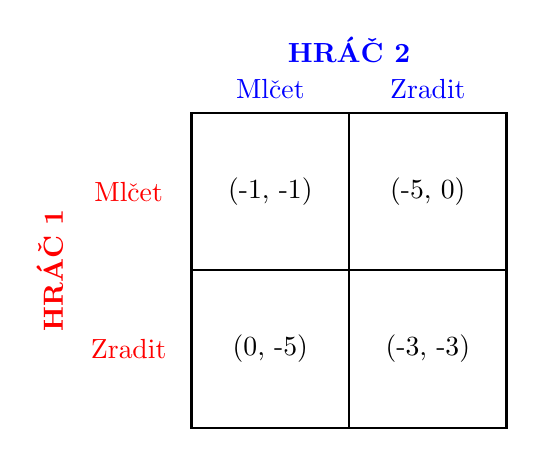
\begin{tikzpicture}
        % Mřížka matice
        \draw[thick] (0,0) rectangle (4,4);
        \draw[thick] (2,0) -- (2,4);
        \draw[thick] (0,2) -- (4,2);

        % Výplaty (Vězňovo dilema)
        \node at (1, 3) {(-1, -1)};
        \node at (3, 3) {(-5, 0)};
        \node at (1, 1) {(0, -5)};
        \node at (3, 1) {(-3, -3)};

        % Hlavičky sloupců (Hráč 2)
        \node[blue] at (1, 4.3) {Mlčet};
        \node[blue] at (3, 4.3) {Zradit};
        \node[blue, font=\bfseries] at (2, 4.8) {HRÁČ 2};

        % Hlavičky řádků (Hráč 1)
        \node[red] at (-0.8, 3) {Mlčet};
        \node[red] at (-0.8, 1) {Zradit};
        \node[red, font=\bfseries, rotate=90] at (-1.8, 2) {HRÁČ 1};
    \end{tikzpicture}
    \caption{Maticová reprezentace (Normální tvar) na příkladu Vězňova dilematu. Červená odpovídá řádkům, modrá sloupcům.}
\end{figure}

\paragraph*{2. Stromová reprezentace (Hra v explicitním tvaru)}
Používá se pro \textbf{sekvenční hry}, kde se hráči v tazích střídají a reagují na sebe.
\begin{itemize}
    \item \textbf{Uzly:} Rozhodovací body. Každý uzel patří konkrétnímu hráči, který je zrovna na tahu. (Kořen stromu je první tah hry).
    \item \textbf{Hrany:} Možné tahy (akce), které má hráč v daném uzlu k dispozici.
    \item \textbf{Listy (Koncové body):} Konec hry, u kterého jsou vypsány výplaty $(v_1, v_2)$ pro všechny hráče.
\end{itemize}

\begin{figure}[htbp]
    \centering
    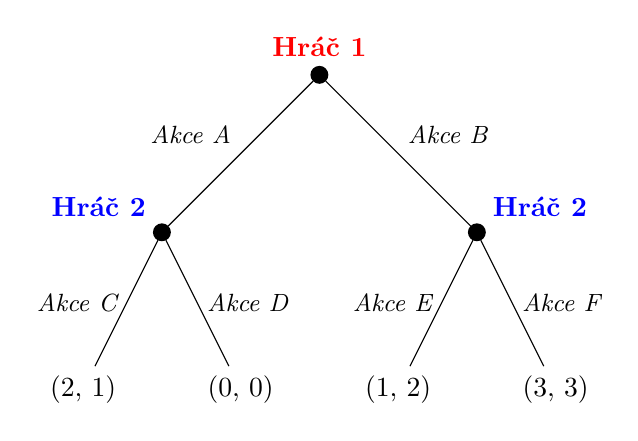
\begin{tikzpicture}[
        level 1/.style={sibling distance=4cm},
        level 2/.style={sibling distance=2cm},
        level distance=2cm,
        player_node/.style={circle, draw, thick, inner sep=2pt, fill=black},
        edge_label/.style={font=\small\itshape}
    ]
        % Kořen - Hráč 1
        \node[player_node, label=above:{\textcolor{red}{\textbf{Hráč 1}}}] {}
            % Tah Vlevo
            child { node[player_node, label=above left:{\textcolor{blue}{\textbf{Hráč 2}}}] {}
                child { node {(2, 1)} edge from parent node[left, edge_label] {Akce C} }
                child { node {(0, 0)} edge from parent node[right, edge_label] {Akce D} }
                edge from parent node[above left, edge_label] {Akce A}
            }
            % Tah Vpravo
            child { node[player_node, label=above right:{\textcolor{blue}{\textbf{Hráč 2}}}] {}
                child { node {(1, 2)} edge from parent node[left, edge_label] {Akce E} }
                child { node {(3, 3)} edge from parent node[right, edge_label] {Akce F} }
                edge from parent node[above right, edge_label] {Akce B}
            };
    \end{tikzpicture}
    \caption{Stromová reprezentace (Explicitní tvar). Nejdříve táhne Hráč 1 (vybírá A nebo B), na jeho volbu pak reaguje Hráč~2.}
\end{figure}

\subsection{Řešení maticových her a Nashova rovnováha}

\paragraph*{1. Eliminace dominovaných strategií}
Než začneme hru složitě řešit, je často možné ji zjednodušit vyřazením nelogických tahů.
\begin{itemize}
    \item \textbf{Dominovaná strategie:} Strategie $A$ je pro hráče (striktně) dominovaná strategií $B$, pokud mu strategie $B$ přináší vždy lepší výplatu bez ohledu na to, co zahraje soupeř.
    \item \textbf{Princip iterativní eliminace:} Protože předpokládáme, že hráči jsou racionální, nikdy nezahrají dominovanou strategii. Můžeme ji tedy z matice (vyškrtnutím řádku nebo sloupce) odstranit. Tím se hra zmenší a tento proces můžeme střídavě opakovat pro oba hráče, dokud nezbude matice, kterou už zredukovat nelze.
\end{itemize}

\paragraph*{2. Nashova rovnováha (NE - Nash Equilibrium)}
\begin{itemize}
    \item \textbf{Definice:} Jedná se o takovou kombinaci strategií (stav hry), ve které žádný z hráčů nemůže jednostrannou změnou své strategie svůj zisk zvýšit. Hráči hrají vůči sobě vzájemně \textit{nejlepší odpovědi}.
    \item \textbf{Hledání v matici (Metoda podtrhávání):} 
    \begin{enumerate}
        \item Postupně zafixujeme sloupce (představíme si, že Hráč 2 zahrál tento tah) a podtrhneme v tomto sloupci nejvyšší výplatu pro Hráče 1.
        \item Postupně zafixujeme řádky (tah Hráče 1) a podtrhneme v něm nejvyšší výplatu pro Hráče~2.
        \item Buňka, ve které jsou podtrženy obě výplaty, je Nashovou rovnováhou v \textit{čistých strategiích}.
    \end{enumerate}
    \item \textbf{Nashova věta:} Každá konečná hra má alespoň jednu Nashovu rovnováhu. Pokud neexistuje v čistých strategiích (např. Kámen-Nůžky-Papír nemá žádnou buňku se dvěma podtržítky), garantovaně existuje ve \textit{smíšených strategiích} (pomocí pravděpodobností).
\end{itemize}

\paragraph*{3. Řešení hry s nulovým součtem}
Jelikož platí $v_1 + v_2 = 0$, zájmy hráčů jsou přesně opačné. Cokoliv Hráč 1 získá, to Hráč 2 ztratí. V matici se proto často uvádí jen výplata Hráče 1. K řešení se využívá \textbf{Minimaxový teorém} (John von Neumann):
\begin{itemize}
    \item \textbf{Maximin Hráče 1 (Dolní cena hry):} Hráč 1 hledá tah, který mu zaručí největší možný zisk za předpokladu, že Hráč 2 bude hrát pro něj co nejhůře. (Maximalizuje své minimální zisky).
    \item \textbf{Minimax Hráče 2 (Horní cena hry):} Hráč 2 chce minimalizovat zisk Hráče 1. Hledá tah, kde Hráč 1 získá co nejméně v nejhorším případě. (Minimalizuje maximální ztráty).
    \item \textbf{Sedlový bod:} Pokud se Maximin = Minimax, hra má řešení v čistých strategiích. Tato společná hodnota se nazývá \textbf{cena hry}. (Sedlový bod je v hrách s nulovým součtem totožný s Nashovou rovnováhou).
    \item Pokud se Maximin $\neq$ Minimax, sedlový bod neexistuje a hra se řeší ve smíšených strategiích pomocí lineárního programování (nebo graficky pro matice $2 \times n$).
\end{itemize}

\begin{figure}[htbp]
    \centering
    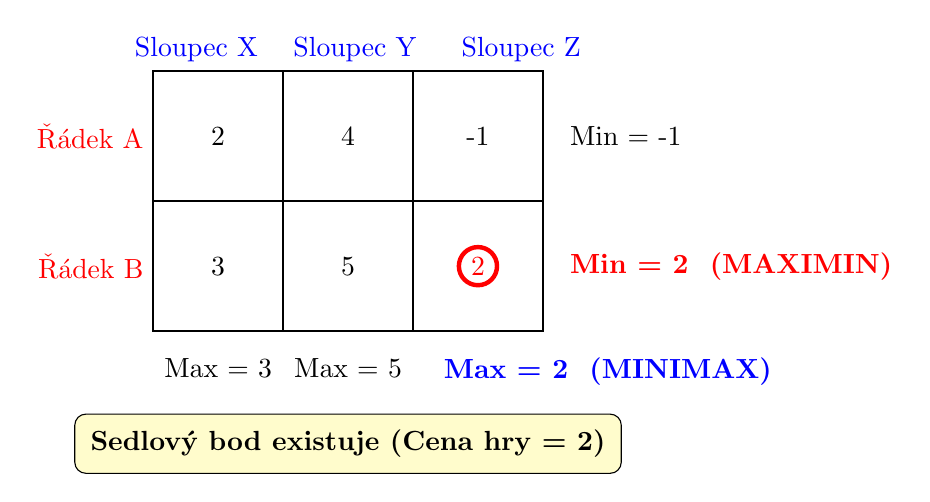
\begin{tikzpicture}[scale=1.1]
        % Mřížka matice 2x3
        \draw[thick] (0,0) rectangle (4.5, 3);
        \draw[thick] (1.5,0) -- (1.5,3);
        \draw[thick] (3,0) -- (3,3);
        \draw[thick] (0,1.5) -- (4.5,1.5);

        % Hlavičky řádků a sloupců
        \node[red, left] at (0, 2.25) {Řádek A};
        \node[red, left] at (0, 0.75) {Řádek B};
        \node[blue, above] at (0.5, 3) {Sloupec X};
        \node[blue, above] at (2.33, 3) {Sloupec Y};
        \node[blue, above] at (4.25, 3) {Sloupec Z};

        % Hodnoty v buňkách (Výplata pro Řádkového hráče)
        \node at (0.75, 2.25) {2};
        \node at (2.25, 2.25) {4};
        \node at (3.75, 2.25) {-1};

        \node at (0.75, 0.75) {3};
        \node at (2.25, 0.75) {5};
        % Sedlový bod zakroužkujeme
        \node[draw, circle, red, ultra thick, inner sep=2pt] at (3.75, 0.75) {2}; 

        % Nalezení řádkových minim
        \node[right] at (4.7, 2.25) {Min = -1};
        \node[right, red, font=\bfseries] at (4.7, 0.75) {Min = 2 \ (MAXIMIN)};

        % Nalezení sloupcových maxim
        \node[below] at (0.75, -0.2) {Max = 3};
        \node[below] at (2.25, -0.2) {Max = 5};
        \node[below, blue, font=\bfseries] at (5.25, -0.2) {Max = 2 \ (MINIMAX)};

        % Závěr
        \node[align=center, font=\bfseries, fill=yellow!20, draw, rounded corners, inner sep=2mm] 
        at (2.25, -1.3) {Sedlový bod existuje (Cena hry = 2)};
    \end{tikzpicture}
    \caption{Řešení hry s nulovým součtem. Maximin řádkového hráče je roven Minimaxu sloupcového hráče, hra má tedy čisté řešení.}
\end{figure}

\paragraph*{4. Řešení hry s nenulovým součtem}
Hráči nejsou absolutní nepřátelé, existuje zde prostor pro oboustranný zisk nebo oboustrannou ztrátu.
\begin{itemize}
    \item Hra se řeší hledáním Nashových rovnováh (kterých může být více).
    \item \textbf{Konflikt s Pareto efektivitou:} Zásadním problémem těchto her je, že Nashova rovnováha nemusí být globálně optimální. Klasickým příkladem je \textit{Vězňovo dilema} - racionální postup oba hráče neomylně dovede do Nashovy rovnováhy (Zradit, Zradit), která je ale pro oba prokazatelně horší než varianta (Mlčet, Mlčet). K lepší variantě se však bez možnosti \textit{závazné dohody} (kooperace) nedostanou, protože samostatně by pro každého bylo výhodné dohodu porušit.
\end{itemize}

\begin{figure}[htbp]
    \centering
    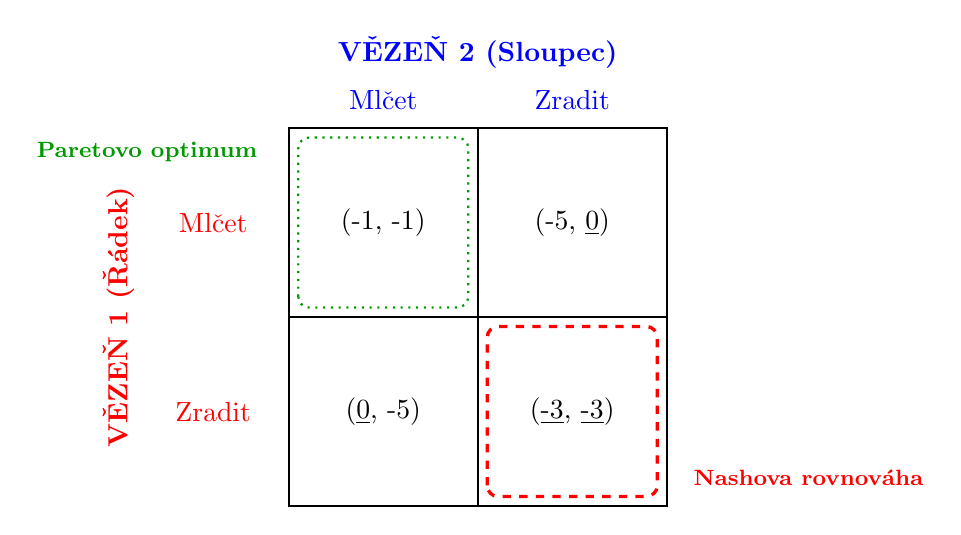
\begin{tikzpicture}[scale=1.2]
        % Mřížka matice
        \draw[thick] (0,0) rectangle (4,4);
        \draw[thick] (2,0) -- (2,4);
        \draw[thick] (0,2) -- (4,2);

        % Hlavičky
        \node[blue, font=\bfseries] at (2, 4.8) {VĚZEŇ 2 (Sloupec)};
        \node[blue] at (1, 4.3) {Mlčet};
        \node[blue] at (3, 4.3) {Zradit};

        \node[red, font=\bfseries, rotate=90] at (-1.8, 2) {VĚZEŇ 1 (Řádek)};
        \node[red] at (-0.8, 3) {Mlčet};
        \node[red] at (-0.8, 1) {Zradit};

        % Výplaty (Záporná čísla znamenají roky ve vězení)
        % V1 mlčí, V2 mlčí
        \node at (1, 3) {(-1, -1)};
        
        % V1 mlčí, V2 zradí -> V1 dostane 5 let, V2 jde na svobodu (0) -> Podtrhneme 0
        \node at (3, 3) {(-5, \underline{0})};
        
        % V1 zradí, V2 mlčí -> V1 jde na svobodu (0), V2 dostane 5 let -> Podtrhneme 0
        \node at (1, 1) {(\underline{0}, -5)};
        
        % Oba zradí -> Oba dostanou 3 roky. Podtrhneme obě výplaty -> Nashova rovnováha!
        \node at (3, 1) {(\underline{-3}, \underline{-3})};

        % Zvýraznění Nashovy rovnováhy
        \draw[red, very thick, dashed, rounded corners] (2.1, 0.1) rectangle (3.9, 1.9);
        \node[red, font=\footnotesize\bfseries] at (5.5, 0.3) {Nashova rovnováha};
        
        % Zvýraznění Paretova optima (Logicky lepší stav, ale matematicky nestabilní)
        \draw[green!60!black, thick, dotted, rounded corners] (0.1, 2.1) rectangle (1.9, 3.9);
        \node[green!60!black, font=\footnotesize\bfseries] at (-1.5, 3.75) {Paretovo optimum};
    \end{tikzpicture}
    \caption{Řešení Vězňova dilematu. Podtržené hodnoty označují nejlepší odpověď hráče na tah soupeře. Červená buňka se dvěma podtržítky je stabilní Nashova rovnováha.}
\end{figure}

\subsection{Řešení hry s rizikem a neurčitostí (Hry proti přírodě)}
Tyto modely nepopisují standardní konflikt dvou racionálních protivníků, ale situaci, kdy jeden racionální hráč činí rozhodnutí vůči prostředí tzv. \textbf{Přírodě}. Příroda nesleduje žádný cíl a nesnaží se hráče poškodit. Její tahy jsou dány pouze náhodou.

\paragraph*{1. Rozhodování za rizika}
Hráč předem zná všechny možné stavy přírody a zná i pravděpodobnosti, se kterými tyto stavy nastanou (např. pravděpodobnost, že bude zítra pršet, je 30\,\%).
\begin{itemize}
    \item \textbf{Pravidlo očekávané hodnoty:} K řešení se využívá výpočet střední hodnoty. Hráč pro každou svou strategii sečte součiny možných výplat a jejich pravděpodobností. Racionální hráč volí tu strategii, která maximalizuje celkový očekávaný zisk.
\end{itemize}

\begin{figure}[h]
    \centering
    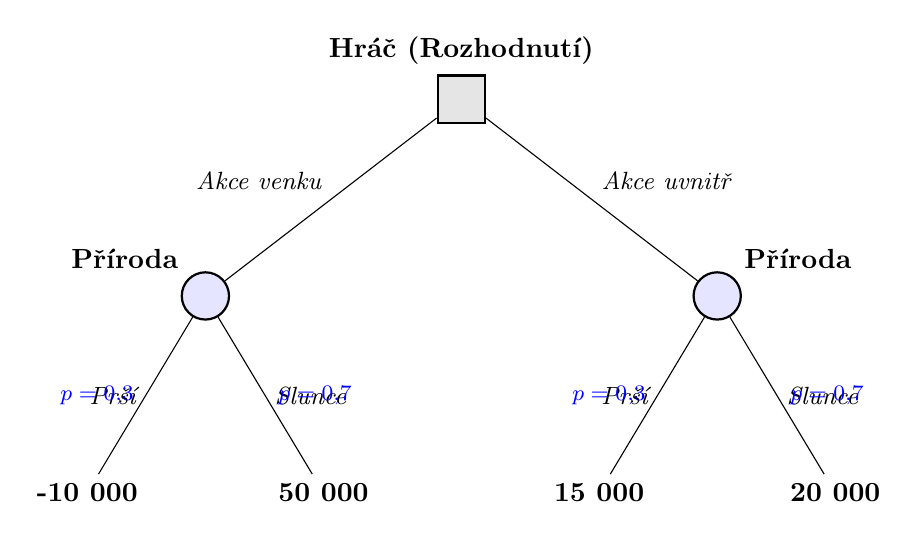
\begin{tikzpicture}[
        level 1/.style={sibling distance=6.5cm},
        level 2/.style={sibling distance=3cm},
        level distance=2.5cm,
        decision_node/.style={rectangle, draw, thick, minimum size=6mm, fill=gray!20},
        chance_node/.style={circle, draw, thick, minimum size=6mm, fill=blue!10},
        edge_label/.style={font=\small\itshape},
        prob_label/.style={font=\footnotesize, text=blue}
    ]
        % Kořen - Rozhodnutí hráče (čtverec)
        \node[decision_node, label=above:{\textbf{Hráč (Rozhodnutí)}}] {}
            % Varianta A (Venku)
            child { node[chance_node, label=above left:{\textbf{Příroda}}] {}
                child { node {\textbf{-10 000}} edge from parent node[left, edge_label] {Prší} node[left=0.75, prob_label] {$p = 0{,}3$} }
                child { node {\textbf{50 000}} edge from parent node[right, edge_label] {Slunce} node[right=1.25, prob_label] {$p = 0{,}7$} }
                edge from parent node[above left, edge_label] {Akce venku}
            }
            % Varianta B (Uvnitř)
            child { node[chance_node, label=above right:{\textbf{Příroda}}] {}
                child { node {\textbf{15 000}} edge from parent node[left, edge_label] {Prší} node[left=0.75, prob_label] {$p = 0{,}3$} }
                child { node {\textbf{20 000}} edge from parent node[right, edge_label] {Slunce} node[right=1.25, prob_label] {$p = 0{,}7$} }
                edge from parent node[above right, edge_label] {Akce uvnitř}
            };
    \end{tikzpicture}
    \caption{Rozhodovací strom pro hru za rizika. Čtvercový uzel značí vědomé rozhodnutí hráče, kruhové uzly představují tahy Přírody (náhodné jevy se známou pravděpodobností $p$). Očekávaná hodnota pro akci venku je $E(V) = 0{,}3 \cdot (-10\,000) + 0{,}7 \cdot 50\,000 = 32\,000$. Očekávaná hodnota pro akci uvnitř je $E(U) = 0{,}3 \cdot 15\,000 + 0{,}7 \cdot 20\,000 = 18\,500$. Racionální hráč volí akci venku, protože maximalizuje očekávaný zisk.}
\end{figure}

\paragraph*{2. Rozhodování za neurčitosti}
Hráč zná všechny možné budoucí stavy přírody, ale nezná pravděpodobnosti jejich výskytu, případně je vůbec nelze odhadnout. Hra se řeší pomocí různých rozhodovacích kritérií na základě toho, jaký postoj má hráč k riziku:
\newpage
\begin{table}[h]
    \centering
    \renewcommand{\arraystretch}{1.3}
    \begin{tabular}{|p{4cm}|p{6cm}|p{5.5cm}|}
        \hline
        \textbf{Kritérium} & \textbf{Postup výběru} & \textbf{Charakteristika} \\ 
        \hline
        \textbf{Princip minimaxu} & Z nejhorších možných výsledků strategií vybere ten nejlepší. & Absolutní pesimista (minimalizuje ztráty, hraje na jistotu). \\ 
        \hline
        \textbf{Princip optimismu racionálního hráče (Hurwiczovo)} & Vážený průměr nejhoršího a nejlepšího výsledku pro každou strategii. & Kompromisní. Využívá koeficient optimismu $\alpha$, kde $0 \le \alpha \le 1$. \\ 
        \hline
        \textbf{Princip minimaxu ztráty (Savageovo)} & Pojistí hráče proti velkým ztrátám oproti optimálnímu rozhodnutí (kdyby strategii
přírody znal předem). & Minimalizuje ušlý zisk. Řeší se pomocí pomocné ztrát a v ní se hledá minimax. \\ 
        \hline
        \textbf{Laplaceovo} & Spočítá prostý aritmetický průměr výplat každé strategie a vybere nejvyšší jako u rizika. & Princip nedostatečného důvodu (předpokládá, že všechny stavy mají stejnou šanci). \\ 
        \hline
    \end{tabular}
\end{table}

\subsection{Řešení hry s neúplnou informací}
Ve hrách s neúplnou informací hráči neznají výplatní funkce (cíle, motivace nebo možnosti) ostatních účastníků. Hráč tedy neví přesně, proti komu hraje, nebo jak moc si soupeř cení výhry. Typickým příkladem jsou aukce, pohovory nebo utajená obchodní vyjednávání.

\paragraph*{1. Harsanyiho transformace}
Americký ekonom John Harsanyi vyřešil problém neúplných informací tím, že do hry zavedl Přírodu jako úvodního hybatele. 
\begin{itemize}
    \item \textbf{Určení typů:} Hra začíná nultým tahem, ve kterém Příroda náhodně vylosuje \textbf{typ} pro každého hráče (např. agresivní konkurent vs. opatrný konkurent).
    \item \textbf{Změna informací:} Každý hráč následně zjistí svůj vlastní typ, ale u soupeřů zná pouze \textit{rozdělení pravděpodobnosti}, s jakou mohou být různými typy.
    \item \textbf{Výsledek:} Původní hra s \textit{neúplnou} informací se matematicky převede na řešitelnou hru s \textit{nedokonalou} (ale už úplnou) informací.
\end{itemize}

\paragraph*{2. Bayesovská Nashova rovnováha}
Protože hráči nevědí s jistotou, jaký typ soupeře proti nim stojí, nemohou hrát klasickou nejlepší odpověď na jeden konkrétní tah. Hledá se proto Bayesovská rovnováha.
\begin{itemize}
    \item \textbf{Princip:} Hráč musí zvážit všechny možné typy svého soupeře, vynásobit jejich tahy pravděpodobností jejich výskytu a podle toho maximalizovat svůj očekávaný užitek. 
    \item Rovnováhy je dosaženo v momentě, kdy je strategie každého hráče tou nejlepší možnou odpovědí na očekávané chování všech ostatních hráčů napříč všemi jejich myslitelnými typy.
\end{itemize}

\begin{quote}
    \textbf{Poznámka:} Každá konečná hra s neúplnou informací má alespoň jedno Bayesovo-Nashovo
rovnovážné řešení.
\end{quote}